\documentclass[final]{scrreprt} %scrreprt of scrartcl
% Include all project wide packages here.
\usepackage{fullpage}
\usepackage{polyglossia}
\setmainlanguage{english}
\usepackage{csquotes}
\usepackage{graphicx}
\usepackage{epstopdf}
\usepackage{pdfpages}
\usepackage{caption}
\usepackage[list=true]{subcaption}
\usepackage{float}
\usepackage{standalone}
\usepackage{import}
\usepackage{tocloft}
\usepackage{wrapfig}
\usepackage{authblk}
\usepackage{array}
\usepackage{booktabs}
\usepackage[toc,page,title,titletoc]{appendix}
\usepackage{xunicode}
\usepackage{fontspec}
\usepackage{pgfplots}
\usepackage{SIunits}
\usepackage{units}
\pgfplotsset{compat=newest}
\pgfplotsset{plot coordinates/math parser=false}
\newlength\figureheight 
\newlength\figurewidth
\usepackage{amsmath}
\usepackage{mathtools}
\usepackage{unicode-math}
\usepackage[
    backend=bibtexu,
	texencoding=utf8,
bibencoding=utf8,
    style=ieee,
    sortlocale=en_US,
    language=auto
]{biblatex}
\usepackage{listings}
\newcommand{\includecode}[3][c]{\lstinputlisting[caption=#2, escapechar=, style=#1]{#3}}
\newcommand{\superscript}[1]{\ensuremath{^{\textrm{#1}}}}
\newcommand{\subscript}[1]{\ensuremath{_{\textrm{#1}}}}


\newcommand{\chapternumber}{\thechapter}
\renewcommand{\appendixname}{Bijlage}
\renewcommand{\appendixtocname}{Bijlagen}
\renewcommand{\appendixpagename}{Bijlagen}

\usepackage[hidelinks]{hyperref} %<--------ALTIJD ALS LAATSTE

\renewcommand{\familydefault}{\sfdefault}

\setmainfont[Ligatures=TeX]{Myriad Pro}
\setmathfont{Asana Math}
\setmonofont{Lucida Console}

\usepackage{titlesec, blindtext, color}
\definecolor{gray75}{gray}{0.75}
\newcommand{\hsp}{\hspace{20pt}}
\titleformat{\chapter}[hang]{\Huge\bfseries}{\chapternumber\hsp\textcolor{gray75}{|}\hsp}{0pt}{\Huge\bfseries}
\renewcommand{\familydefault}{\sfdefault}
\renewcommand{\arraystretch}{1.2}
\setlength\parindent{0pt}

%For code listings
\definecolor{black}{rgb}{0,0,0}
\definecolor{browntags}{rgb}{0.65,0.1,0.1}
\definecolor{bluestrings}{rgb}{0,0,1}
\definecolor{graycomments}{rgb}{0.4,0.4,0.4}
\definecolor{redkeywords}{rgb}{1,0,0}
\definecolor{bluekeywords}{rgb}{0.13,0.13,0.8}
\definecolor{greencomments}{rgb}{0,0.5,0}
\definecolor{redstrings}{rgb}{0.9,0,0}
\definecolor{purpleidentifiers}{rgb}{0.01,0,0.01}


\lstdefinestyle{csharp}{
language=[Sharp]C,
showspaces=false,
showtabs=false,
breaklines=true,
showstringspaces=false,
breakatwhitespace=true,
escapeinside={(*@}{@*)},
columns=fullflexible,
commentstyle=\color{greencomments},
keywordstyle=\color{bluekeywords}\bfseries,
stringstyle=\color{redstrings},
identifierstyle=\color{purpleidentifiers},
basicstyle=\ttfamily\small}

\lstdefinestyle{c}{
language=C,
showspaces=false,
showtabs=false,
breaklines=true,
showstringspaces=false,
breakatwhitespace=true,
escapeinside={(*@}{@*)},
columns=fullflexible,
commentstyle=\color{greencomments},
keywordstyle=\color{bluekeywords}\bfseries,
stringstyle=\color{redstrings},
identifierstyle=\color{purpleidentifiers},
}

\lstdefinestyle{matlab}{
language=Matlab,
showspaces=false,
showtabs=false,
breaklines=true,
showstringspaces=false,
breakatwhitespace=true,
escapeinside={(*@}{@*)},
columns=fullflexible,
commentstyle=\color{greencomments},
keywordstyle=\color{bluekeywords}\bfseries,
stringstyle=\color{redstrings},
identifierstyle=\color{purpleidentifiers}
}

\lstdefinestyle{vhdl}{
language=VHDL,
showspaces=false,
showtabs=false,
breaklines=true,
showstringspaces=false,
breakatwhitespace=true,
escapeinside={(*@}{@*)},
columns=fullflexible,
commentstyle=\color{greencomments},
keywordstyle=\color{bluekeywords}\bfseries,
stringstyle=\color{redstrings},
identifierstyle=\color{purpleidentifiers}
}

\lstdefinestyle{xaml}{
language=XML,
showspaces=false,
showtabs=false,
breaklines=true,
showstringspaces=false,
breakatwhitespace=true,
escapeinside={(*@}{@*)},
columns=fullflexible,
commentstyle=\color{greencomments},
keywordstyle=\color{redkeywords},
stringstyle=\color{bluestrings},
tagstyle=\color{browntags},
morestring=[b]",
  morecomment=[s]{<?}{?>},
  morekeywords={xmlns,version,typex:AsyncRecords,x:Arguments,x:Boolean,x:Byte,x:Char,x:Class,x:ClassAttributes,x:ClassModifier,x:Code,x:ConnectionId,x:Decimal,x:Double,x:FactoryMethod,x:FieldModifier,x:Int16,x:Int32,x:Int64,x:Key,x:Members,x:Name,x:Object,x:Property,x:Shared,x:Single,x:String,x:Subclass,x:SynchronousMode,x:TimeSpan,x:TypeArguments,x:Uid,x:Uri,x:XData,Grid.Column,Grid.ColumnSpan,Click,ClipToBounds,Content,DropDownOpened,FontSize,Foreground,Header,Height,HorizontalAlignment,HorizontalContentAlignment,IsCancel,IsDefault,IsEnabled,IsSelected,Margin,MinHeight,MinWidth,Padding,SnapsToDevicePixels,Target,TextWrapping,Title,VerticalAlignment,VerticalContentAlignment,Width,WindowStartupLocation,Binding,Mode,OneWay,xmlns:x}
}

%defaults
\lstset{
basicstyle=\ttfamily\small,
extendedchars=false,
numbers=left,
numberstyle=\ttfamily\tiny,
stepnumber=1,
tabsize=4,
numbersep=5pt
}
\addbibresource{../../library/bibliography.bib}

\begin{document}
\section*{Labday 1: Basic filtering in time domain and frequency domain}
\subsection*{Report 1: Channel impulse response}
In a 2-dimensional room of 4x4 m, a transmitter and a receiver are placed at (1.2, 0.3) and (3.1, 3.3) resp.
The propagation of a delta impulse from TX to RX is being investigated with the use of the following equation:

\begin{equation}
	\alpha (r) = \frac{\beta}{r^2}
\label{eq:damping}
\end{equation}

where $\beta$ is the damping over a reference distance of 1 meter.
\\ \\
The direct path is fastest and strongest at the RX point and can be calculated directly.
The indirect paths, as a result of reflections, can be calculated by looking at the mirror images of the TX and RX over the edges of the room.
For the first order reflections, only one mirror image is needed of either the RX or TX.
We choose to mirror the RX.
The mirrored image of the TX and the original RX are connected, which always results in an intersection with a wall.
Since there are four walls, four virtual sources are created this way when looking at first order reflections.
This location at the wall is the point where the single bounce is made, connecting this point with both the RX and TX will be the total path.
\\ \\
Second order reflections are calculated by mirroring both the TX and RX as displayed in Figure \ref{fig:mirror}.
Note that also the first order reflections are displayed in this figure since the TX is also present as non-mirrored version.
The connection between the mirror images might intersect with the room.
The connection either intersects with two walls or none, since both mirror images are outside the room.
When there are intersections, the two points on the two different walls are the two points via which the delta impulse bounces exactly to the RX from the TX.
The TX and RX are mirrored over all walls in all 16 combinations, but not all of them intersect with the room, which states that it is not possible to bounce via this two walls.
By inspecting Figure \ref{fig:connected}, it is clear that only 8 paths of the total 16 are possible, making 8 virtual sources from second order reflections.
\\ \\
The second order reflection paths are drawn by connecting the two wall intersections, the RX with the intersection at the wall it was reflected over and the TX with the intersection at its wall.
When the length of all direct and reflected paths are measured and using the speed of sound, the delay of each path can be calculated.
Also, using Eq. \ref{eq:damping}, the resulting amplitude can be calculated.
We used a $\beta$ of 1.00 since the outcome of all amplitudes would give the total received signal compared to a infinitely large room with the TX and RX 1 meter from each other.
The resulting delta impulse response over time is displayed in Figure \ref{fig:response}.
Using the Matlab script from Appendix A, a resulting total amplitude of 0.5420, which equals the sum of all delta impulse response amplitudes from Figure \ref{fig:response}.

\begin{figure}[H]
	\centering
	\setlength\figureheight{6cm}
    	\setlength\figurewidth{6cm}
	% This file was created by matlab2tikz v0.4.6 running on MATLAB 8.2.
% Copyright (c) 2008--2014, Nico Schlömer <nico.schloemer@gmail.com>
% All rights reserved.
% Minimal pgfplots version: 1.3
% 
% The latest updates can be retrieved from
%   http://www.mathworks.com/matlabcentral/fileexchange/22022-matlab2tikz
% where you can also make suggestions and rate matlab2tikz.
% 
\begin{tikzpicture}

\begin{axis}[%
width=\figurewidth,
height=\figureheight,
scale only axis,
xmin=-4,
xmax=8,
xlabel={x location (m)},
ymin=-4,
ymax=8,
ylabel={y location (m)},
axis x line*=bottom,
axis y line*=left
]
\addplot [color=blue,only marks,mark=asterisk,mark options={solid},forget plot]
  table[row sep=crcr]{
1.2	0.3	\\
};
\addplot [color=blue,only marks,mark=asterisk,mark options={solid},forget plot]
  table[row sep=crcr]{
3.1	3.3	\\
};
\addplot [color=blue,solid,forget plot]
  table[row sep=crcr]{
0	0	\\
0	4	\\
};
\addplot [color=blue,solid,forget plot]
  table[row sep=crcr]{
4	4	\\
0	4	\\
};
\addplot [color=blue,solid,forget plot]
  table[row sep=crcr]{
4	0	\\
0	0	\\
};
\addplot [color=blue,solid,forget plot]
  table[row sep=crcr]{
4	4	\\
4	0	\\
};
\addplot [color=red,only marks,mark=asterisk,mark options={solid},forget plot]
  table[row sep=crcr]{
3.1	4.7	\\
};
\addplot [color=red,only marks,mark=asterisk,mark options={solid},forget plot]
  table[row sep=crcr]{
4.9	3.3	\\
};
\addplot [color=red,only marks,mark=asterisk,mark options={solid},forget plot]
  table[row sep=crcr]{
3.1	-3.3	\\
};
\addplot [color=red,only marks,mark=asterisk,mark options={solid},forget plot]
  table[row sep=crcr]{
-3.1	3.3	\\
};
\addplot [color=red,only marks,mark=asterisk,mark options={solid},forget plot]
  table[row sep=crcr]{
4.9	3.3	\\
};
\addplot [color=red,only marks,mark=asterisk,mark options={solid},forget plot]
  table[row sep=crcr]{
1.2	7.7	\\
};
\addplot [color=red,only marks,mark=asterisk,mark options={solid},forget plot]
  table[row sep=crcr]{
3.1	-3.3	\\
};
\addplot [color=red,only marks,mark=asterisk,mark options={solid},forget plot]
  table[row sep=crcr]{
1.2	7.7	\\
};
\addplot [color=red,only marks,mark=asterisk,mark options={solid},forget plot]
  table[row sep=crcr]{
-3.1	3.3	\\
};
\addplot [color=red,only marks,mark=asterisk,mark options={solid},forget plot]
  table[row sep=crcr]{
1.2	7.7	\\
};
\addplot [color=red,only marks,mark=asterisk,mark options={solid},forget plot]
  table[row sep=crcr]{
3.1	4.7	\\
};
\addplot [color=red,only marks,mark=asterisk,mark options={solid},forget plot]
  table[row sep=crcr]{
6.8	0.3	\\
};
\addplot [color=red,only marks,mark=asterisk,mark options={solid},forget plot]
  table[row sep=crcr]{
3.1	-3.3	\\
};
\addplot [color=red,only marks,mark=asterisk,mark options={solid},forget plot]
  table[row sep=crcr]{
6.8	0.3	\\
};
\addplot [color=red,only marks,mark=asterisk,mark options={solid},forget plot]
  table[row sep=crcr]{
-3.1	3.3	\\
};
\addplot [color=red,only marks,mark=asterisk,mark options={solid},forget plot]
  table[row sep=crcr]{
6.8	0.3	\\
};
\addplot [color=red,only marks,mark=asterisk,mark options={solid},forget plot]
  table[row sep=crcr]{
3.1	4.7	\\
};
\addplot [color=red,only marks,mark=asterisk,mark options={solid},forget plot]
  table[row sep=crcr]{
1.2	-0.3	\\
};
\addplot [color=red,only marks,mark=asterisk,mark options={solid},forget plot]
  table[row sep=crcr]{
4.9	3.3	\\
};
\addplot [color=red,only marks,mark=asterisk,mark options={solid},forget plot]
  table[row sep=crcr]{
1.2	-0.3	\\
};
\addplot [color=red,only marks,mark=asterisk,mark options={solid},forget plot]
  table[row sep=crcr]{
-3.1	3.3	\\
};
\addplot [color=red,only marks,mark=asterisk,mark options={solid},forget plot]
  table[row sep=crcr]{
1.2	-0.3	\\
};
\addplot [color=red,only marks,mark=asterisk,mark options={solid},forget plot]
  table[row sep=crcr]{
3.1	4.7	\\
};
\addplot [color=red,only marks,mark=asterisk,mark options={solid},forget plot]
  table[row sep=crcr]{
-1.2	0.3	\\
};
\addplot [color=red,only marks,mark=asterisk,mark options={solid},forget plot]
  table[row sep=crcr]{
4.9	3.3	\\
};
\addplot [color=red,only marks,mark=asterisk,mark options={solid},forget plot]
  table[row sep=crcr]{
-1.2	0.3	\\
};
\addplot [color=red,only marks,mark=asterisk,mark options={solid},forget plot]
  table[row sep=crcr]{
3.1	-3.3	\\
};
\addplot [color=red,only marks,mark=asterisk,mark options={solid},forget plot]
  table[row sep=crcr]{
-1.2	0.3	\\
};
\end{axis}
\end{tikzpicture}%
	\caption{Mirror images of the TX and RX.}
	\label{fig:mirror}
\end{figure}

\begin{figure}[H]
	\centering
	\setlength\figureheight{6cm}
    	\setlength\figurewidth{6cm}
	% This file was created by matlab2tikz v0.4.6 running on MATLAB 8.2.
% Copyright (c) 2008--2014, Nico Schlömer <nico.schloemer@gmail.com>
% All rights reserved.
% Minimal pgfplots version: 1.3
% 
% The latest updates can be retrieved from
%   http://www.mathworks.com/matlabcentral/fileexchange/22022-matlab2tikz
% where you can also make suggestions and rate matlab2tikz.
% 
\begin{tikzpicture}

\begin{axis}[%
width=\figurewidth,
height=\figureheight,
scale only axis,
xmin=-4,
xmax=8,
xlabel={x location (m)},
ymin=-4,
ymax=8,
ylabel={y location (m)},
axis x line*=bottom,
axis y line*=left
]
\addplot [color=blue,only marks,mark=asterisk,mark options={solid},forget plot]
  table[row sep=crcr]{
1.2	0.3	\\
};
\addplot [color=blue,only marks,mark=asterisk,mark options={solid},forget plot]
  table[row sep=crcr]{
3.1	3.3	\\
};
\addplot [color=blue,solid,forget plot]
  table[row sep=crcr]{
0	0	\\
0	4	\\
};
\addplot [color=blue,solid,forget plot]
  table[row sep=crcr]{
4	4	\\
0	4	\\
};
\addplot [color=blue,solid,forget plot]
  table[row sep=crcr]{
4	0	\\
0	0	\\
};
\addplot [color=blue,solid,forget plot]
  table[row sep=crcr]{
4	4	\\
4	0	\\
};
\addplot [color=red,only marks,mark=asterisk,mark options={solid},forget plot]
  table[row sep=crcr]{
3.1	4.7	\\
};
\addplot [color=red,dotted,forget plot]
  table[row sep=crcr]{
1.2	0.3	\\
3.1	4.7	\\
};
\addplot [color=red,only marks,mark=asterisk,mark options={solid},forget plot]
  table[row sep=crcr]{
1.2	0.3	\\
};
\addplot [color=red,only marks,mark=asterisk,mark options={solid},forget plot]
  table[row sep=crcr]{
2.79772727272727	4	\\
};
\addplot [color=red,only marks,mark=asterisk,mark options={solid},forget plot]
  table[row sep=crcr]{
4.9	3.3	\\
};
\addplot [color=red,dotted,forget plot]
  table[row sep=crcr]{
1.2	0.3	\\
4.9	3.3	\\
};
\addplot [color=red,only marks,mark=asterisk,mark options={solid},forget plot]
  table[row sep=crcr]{
1.2	0.3	\\
};
\addplot [color=red,only marks,mark=asterisk,mark options={solid},forget plot]
  table[row sep=crcr]{
4	2.57027027027027	\\
};
\addplot [color=red,only marks,mark=asterisk,mark options={solid},forget plot]
  table[row sep=crcr]{
3.1	-3.3	\\
};
\addplot [color=red,dotted,forget plot]
  table[row sep=crcr]{
1.2	0.3	\\
3.1	-3.3	\\
};
\addplot [color=red,only marks,mark=asterisk,mark options={solid},forget plot]
  table[row sep=crcr]{
1.2	0.3	\\
};
\addplot [color=red,only marks,mark=asterisk,mark options={solid},forget plot]
  table[row sep=crcr]{
1.35833333333333	0	\\
};
\addplot [color=red,only marks,mark=asterisk,mark options={solid},forget plot]
  table[row sep=crcr]{
-3.1	3.3	\\
};
\addplot [color=red,dotted,forget plot]
  table[row sep=crcr]{
1.2	0.3	\\
-3.1	3.3	\\
};
\addplot [color=red,only marks,mark=asterisk,mark options={solid},forget plot]
  table[row sep=crcr]{
1.2	0.3	\\
};
\addplot [color=red,only marks,mark=asterisk,mark options={solid},forget plot]
  table[row sep=crcr]{
0	1.13720930232558	\\
};
\addplot [color=red,only marks,mark=asterisk,mark options={solid},forget plot]
  table[row sep=crcr]{
4.9	3.3	\\
};
\addplot [color=red,only marks,mark=asterisk,mark options={solid},forget plot]
  table[row sep=crcr]{
1.2	7.7	\\
};
\addplot [color=red,dotted,forget plot]
  table[row sep=crcr]{
1.2	7.7	\\
4.9	3.3	\\
};
\addplot [color=red,only marks,mark=asterisk,mark options={solid},forget plot]
  table[row sep=crcr]{
3.1	-3.3	\\
};
\addplot [color=red,only marks,mark=asterisk,mark options={solid},forget plot]
  table[row sep=crcr]{
1.2	7.7	\\
};
\addplot [color=red,dotted,forget plot]
  table[row sep=crcr]{
1.2	7.7	\\
3.1	-3.3	\\
};
\addplot [color=red,only marks,mark=asterisk,mark options={solid},forget plot]
  table[row sep=crcr]{
1.83909090909091	4	\\
};
\addplot [color=red,only marks,mark=asterisk,mark options={solid},forget plot]
  table[row sep=crcr]{
2.53	0	\\
};
\addplot [color=red,only marks,mark=asterisk,mark options={solid},forget plot]
  table[row sep=crcr]{
-3.1	3.3	\\
};
\addplot [color=red,only marks,mark=asterisk,mark options={solid},forget plot]
  table[row sep=crcr]{
1.2	7.7	\\
};
\addplot [color=red,dotted,forget plot]
  table[row sep=crcr]{
1.2	7.7	\\
-3.1	3.3	\\
};
\addplot [color=red,only marks,mark=asterisk,mark options={solid},forget plot]
  table[row sep=crcr]{
3.1	4.7	\\
};
\addplot [color=red,only marks,mark=asterisk,mark options={solid},forget plot]
  table[row sep=crcr]{
6.8	0.3	\\
};
\addplot [color=red,dotted,forget plot]
  table[row sep=crcr]{
6.8	0.3	\\
3.1	4.7	\\
};
\addplot [color=red,only marks,mark=asterisk,mark options={solid},forget plot]
  table[row sep=crcr]{
4	3.62972972972973	\\
};
\addplot [color=red,only marks,mark=asterisk,mark options={solid},forget plot]
  table[row sep=crcr]{
3.68863636363636	4	\\
};
\addplot [color=red,only marks,mark=asterisk,mark options={solid},forget plot]
  table[row sep=crcr]{
3.1	-3.3	\\
};
\addplot [color=red,only marks,mark=asterisk,mark options={solid},forget plot]
  table[row sep=crcr]{
6.8	0.3	\\
};
\addplot [color=red,dotted,forget plot]
  table[row sep=crcr]{
6.8	0.3	\\
3.1	-3.3	\\
};
\addplot [color=red,only marks,mark=asterisk,mark options={solid},forget plot]
  table[row sep=crcr]{
-3.1	3.3	\\
};
\addplot [color=red,only marks,mark=asterisk,mark options={solid},forget plot]
  table[row sep=crcr]{
6.8	0.3	\\
};
\addplot [color=red,dotted,forget plot]
  table[row sep=crcr]{
6.8	0.3	\\
-3.1	3.3	\\
};
\addplot [color=red,only marks,mark=asterisk,mark options={solid},forget plot]
  table[row sep=crcr]{
4	1.14848484848485	\\
};
\addplot [color=red,only marks,mark=asterisk,mark options={solid},forget plot]
  table[row sep=crcr]{
0	2.36060606060606	\\
};
\addplot [color=red,only marks,mark=asterisk,mark options={solid},forget plot]
  table[row sep=crcr]{
3.1	4.7	\\
};
\addplot [color=red,only marks,mark=asterisk,mark options={solid},forget plot]
  table[row sep=crcr]{
1.2	-0.3	\\
};
\addplot [color=red,dotted,forget plot]
  table[row sep=crcr]{
1.2	-0.3	\\
3.1	4.7	\\
};
\addplot [color=red,only marks,mark=asterisk,mark options={solid},forget plot]
  table[row sep=crcr]{
1.314	0	\\
};
\addplot [color=red,only marks,mark=asterisk,mark options={solid},forget plot]
  table[row sep=crcr]{
2.834	4	\\
};
\addplot [color=red,only marks,mark=asterisk,mark options={solid},forget plot]
  table[row sep=crcr]{
4.9	3.3	\\
};
\addplot [color=red,only marks,mark=asterisk,mark options={solid},forget plot]
  table[row sep=crcr]{
1.2	-0.3	\\
};
\addplot [color=red,dotted,forget plot]
  table[row sep=crcr]{
1.2	-0.3	\\
4.9	3.3	\\
};
\addplot [color=red,only marks,mark=asterisk,mark options={solid},forget plot]
  table[row sep=crcr]{
1.50833333333333	0	\\
};
\addplot [color=red,only marks,mark=asterisk,mark options={solid},forget plot]
  table[row sep=crcr]{
4	2.42432432432432	\\
};
\addplot [color=red,only marks,mark=asterisk,mark options={solid},forget plot]
  table[row sep=crcr]{
-3.1	3.3	\\
};
\addplot [color=red,only marks,mark=asterisk,mark options={solid},forget plot]
  table[row sep=crcr]{
1.2	-0.3	\\
};
\addplot [color=red,dotted,forget plot]
  table[row sep=crcr]{
1.2	-0.3	\\
-3.1	3.3	\\
};
\addplot [color=red,only marks,mark=asterisk,mark options={solid},forget plot]
  table[row sep=crcr]{
0.841666666666667	0	\\
};
\addplot [color=red,only marks,mark=asterisk,mark options={solid},forget plot]
  table[row sep=crcr]{
0	0.704651162790698	\\
};
\addplot [color=red,only marks,mark=asterisk,mark options={solid},forget plot]
  table[row sep=crcr]{
3.1	4.7	\\
};
\addplot [color=red,only marks,mark=asterisk,mark options={solid},forget plot]
  table[row sep=crcr]{
-1.2	0.3	\\
};
\addplot [color=red,dotted,forget plot]
  table[row sep=crcr]{
-1.2	0.3	\\
3.1	4.7	\\
};
\addplot [color=red,only marks,mark=asterisk,mark options={solid},forget plot]
  table[row sep=crcr]{
0	1.52790697674419	\\
};
\addplot [color=red,only marks,mark=asterisk,mark options={solid},forget plot]
  table[row sep=crcr]{
2.41590909090909	4	\\
};
\addplot [color=red,only marks,mark=asterisk,mark options={solid},forget plot]
  table[row sep=crcr]{
4.9	3.3	\\
};
\addplot [color=red,only marks,mark=asterisk,mark options={solid},forget plot]
  table[row sep=crcr]{
-1.2	0.3	\\
};
\addplot [color=red,dotted,forget plot]
  table[row sep=crcr]{
-1.2	0.3	\\
4.9	3.3	\\
};
\addplot [color=red,only marks,mark=asterisk,mark options={solid},forget plot]
  table[row sep=crcr]{
0	0.89016393442623	\\
};
\addplot [color=red,only marks,mark=asterisk,mark options={solid},forget plot]
  table[row sep=crcr]{
4	2.85737704918033	\\
};
\addplot [color=red,only marks,mark=asterisk,mark options={solid},forget plot]
  table[row sep=crcr]{
3.1	-3.3	\\
};
\addplot [color=red,only marks,mark=asterisk,mark options={solid},forget plot]
  table[row sep=crcr]{
-1.2	0.3	\\
};
\addplot [color=red,dotted,forget plot]
  table[row sep=crcr]{
-1.2	0.3	\\
3.1	-3.3	\\
};
\end{axis}
\end{tikzpicture}%
	\caption{Connected mirror images of the TX and RX.}
	\label{fig:connected}
\end{figure}

\begin{figure}[H]
	\centering
	\setlength\figureheight{6cm}
    	\setlength\figurewidth{6cm}
	% This file was created by matlab2tikz v0.4.6 running on MATLAB 8.2.
% Copyright (c) 2008--2014, Nico Schlömer <nico.schloemer@gmail.com>
% All rights reserved.
% Minimal pgfplots version: 1.3
% 
% The latest updates can be retrieved from
%   http://www.mathworks.com/matlabcentral/fileexchange/22022-matlab2tikz
% where you can also make suggestions and rate matlab2tikz.
% 
\begin{tikzpicture}

\begin{axis}[%
width=\figurewidth,
height=\figureheight,
scale only axis,
xmin=0,
xmax=4,
xlabel={x location (m)},
ymin=0,
ymax=4,
ylabel={y location (m)},
axis x line*=bottom,
axis y line*=left
]
\addplot [color=blue,only marks,mark=asterisk,mark options={solid},forget plot]
  table[row sep=crcr]{
1.2	0.3	\\
};
\addplot [color=blue,only marks,mark=asterisk,mark options={solid},forget plot]
  table[row sep=crcr]{
3.1	3.3	\\
};
\addplot [color=red,solid,forget plot]
  table[row sep=crcr]{
1.2	0.3	\\
3.1	3.3	\\
};
\addplot [color=blue,solid,forget plot]
  table[row sep=crcr]{
0	0	\\
0	4	\\
};
\addplot [color=blue,solid,forget plot]
  table[row sep=crcr]{
4	4	\\
0	4	\\
};
\addplot [color=blue,solid,forget plot]
  table[row sep=crcr]{
4	0	\\
0	0	\\
};
\addplot [color=blue,solid,forget plot]
  table[row sep=crcr]{
4	4	\\
4	0	\\
};
\addplot [color=red,only marks,mark=asterisk,mark options={solid},forget plot]
  table[row sep=crcr]{
1.2	0.3	\\
};
\addplot [color=red,only marks,mark=asterisk,mark options={solid},forget plot]
  table[row sep=crcr]{
2.79772727272727	4	\\
};
\addplot [color=red,solid,forget plot]
  table[row sep=crcr]{
1.2	0.3	\\
1.2	0.3	\\
};
\addplot [color=red,solid,forget plot]
  table[row sep=crcr]{
3.1	3.3	\\
2.79772727272727	4	\\
};
\addplot [color=red,solid,forget plot]
  table[row sep=crcr]{
1.2	0.3	\\
2.79772727272727	4	\\
};
\addplot [color=red,only marks,mark=asterisk,mark options={solid},forget plot]
  table[row sep=crcr]{
1.2	0.3	\\
};
\addplot [color=red,only marks,mark=asterisk,mark options={solid},forget plot]
  table[row sep=crcr]{
4	2.57027027027027	\\
};
\addplot [color=red,solid,forget plot]
  table[row sep=crcr]{
1.2	0.3	\\
1.2	0.3	\\
};
\addplot [color=red,solid,forget plot]
  table[row sep=crcr]{
3.1	3.3	\\
4	2.57027027027027	\\
};
\addplot [color=red,solid,forget plot]
  table[row sep=crcr]{
1.2	0.3	\\
4	2.57027027027027	\\
};
\addplot [color=red,only marks,mark=asterisk,mark options={solid},forget plot]
  table[row sep=crcr]{
1.2	0.3	\\
};
\addplot [color=red,only marks,mark=asterisk,mark options={solid},forget plot]
  table[row sep=crcr]{
1.35833333333333	0	\\
};
\addplot [color=red,solid,forget plot]
  table[row sep=crcr]{
1.2	0.3	\\
1.2	0.3	\\
};
\addplot [color=red,solid,forget plot]
  table[row sep=crcr]{
3.1	3.3	\\
1.35833333333333	0	\\
};
\addplot [color=red,solid,forget plot]
  table[row sep=crcr]{
1.2	0.3	\\
1.35833333333333	0	\\
};
\addplot [color=red,only marks,mark=asterisk,mark options={solid},forget plot]
  table[row sep=crcr]{
1.2	0.3	\\
};
\addplot [color=red,only marks,mark=asterisk,mark options={solid},forget plot]
  table[row sep=crcr]{
0	1.13720930232558	\\
};
\addplot [color=red,solid,forget plot]
  table[row sep=crcr]{
1.2	0.3	\\
1.2	0.3	\\
};
\addplot [color=red,solid,forget plot]
  table[row sep=crcr]{
3.1	3.3	\\
0	1.13720930232558	\\
};
\addplot [color=red,solid,forget plot]
  table[row sep=crcr]{
1.2	0.3	\\
0	1.13720930232558	\\
};
\addplot [color=red,only marks,mark=asterisk,mark options={solid},forget plot]
  table[row sep=crcr]{
1.83909090909091	4	\\
};
\addplot [color=red,only marks,mark=asterisk,mark options={solid},forget plot]
  table[row sep=crcr]{
2.53	0	\\
};
\addplot [color=red,solid,forget plot]
  table[row sep=crcr]{
1.2	0.3	\\
1.83909090909091	4	\\
};
\addplot [color=red,solid,forget plot]
  table[row sep=crcr]{
3.1	3.3	\\
2.53	0	\\
};
\addplot [color=red,solid,forget plot]
  table[row sep=crcr]{
1.83909090909091	4	\\
2.53	0	\\
};
\addplot [color=red,only marks,mark=asterisk,mark options={solid},forget plot]
  table[row sep=crcr]{
4	3.62972972972973	\\
};
\addplot [color=red,only marks,mark=asterisk,mark options={solid},forget plot]
  table[row sep=crcr]{
3.68863636363636	4	\\
};
\addplot [color=red,solid,forget plot]
  table[row sep=crcr]{
1.2	0.3	\\
4	3.62972972972973	\\
};
\addplot [color=red,solid,forget plot]
  table[row sep=crcr]{
3.1	3.3	\\
3.68863636363636	4	\\
};
\addplot [color=red,solid,forget plot]
  table[row sep=crcr]{
4	3.62972972972973	\\
3.68863636363636	4	\\
};
\addplot [color=red,only marks,mark=asterisk,mark options={solid},forget plot]
  table[row sep=crcr]{
4	1.14848484848485	\\
};
\addplot [color=red,only marks,mark=asterisk,mark options={solid},forget plot]
  table[row sep=crcr]{
0	2.36060606060606	\\
};
\addplot [color=red,solid,forget plot]
  table[row sep=crcr]{
1.2	0.3	\\
4	1.14848484848485	\\
};
\addplot [color=red,solid,forget plot]
  table[row sep=crcr]{
3.1	3.3	\\
0	2.36060606060606	\\
};
\addplot [color=red,solid,forget plot]
  table[row sep=crcr]{
4	1.14848484848485	\\
0	2.36060606060606	\\
};
\addplot [color=red,only marks,mark=asterisk,mark options={solid},forget plot]
  table[row sep=crcr]{
1.314	0	\\
};
\addplot [color=red,only marks,mark=asterisk,mark options={solid},forget plot]
  table[row sep=crcr]{
2.834	4	\\
};
\addplot [color=red,solid,forget plot]
  table[row sep=crcr]{
1.2	0.3	\\
1.314	0	\\
};
\addplot [color=red,solid,forget plot]
  table[row sep=crcr]{
3.1	3.3	\\
2.834	4	\\
};
\addplot [color=red,solid,forget plot]
  table[row sep=crcr]{
1.314	0	\\
2.834	4	\\
};
\addplot [color=red,only marks,mark=asterisk,mark options={solid},forget plot]
  table[row sep=crcr]{
1.50833333333333	0	\\
};
\addplot [color=red,only marks,mark=asterisk,mark options={solid},forget plot]
  table[row sep=crcr]{
4	2.42432432432432	\\
};
\addplot [color=red,solid,forget plot]
  table[row sep=crcr]{
1.2	0.3	\\
1.50833333333333	0	\\
};
\addplot [color=red,solid,forget plot]
  table[row sep=crcr]{
3.1	3.3	\\
4	2.42432432432432	\\
};
\addplot [color=red,solid,forget plot]
  table[row sep=crcr]{
1.50833333333333	0	\\
4	2.42432432432432	\\
};
\addplot [color=red,only marks,mark=asterisk,mark options={solid},forget plot]
  table[row sep=crcr]{
0.841666666666667	0	\\
};
\addplot [color=red,only marks,mark=asterisk,mark options={solid},forget plot]
  table[row sep=crcr]{
0	0.704651162790698	\\
};
\addplot [color=red,solid,forget plot]
  table[row sep=crcr]{
1.2	0.3	\\
0.841666666666667	0	\\
};
\addplot [color=red,solid,forget plot]
  table[row sep=crcr]{
3.1	3.3	\\
0	0.704651162790698	\\
};
\addplot [color=red,solid,forget plot]
  table[row sep=crcr]{
0.841666666666667	0	\\
0	0.704651162790698	\\
};
\addplot [color=red,only marks,mark=asterisk,mark options={solid},forget plot]
  table[row sep=crcr]{
0	1.52790697674419	\\
};
\addplot [color=red,only marks,mark=asterisk,mark options={solid},forget plot]
  table[row sep=crcr]{
2.41590909090909	4	\\
};
\addplot [color=red,solid,forget plot]
  table[row sep=crcr]{
1.2	0.3	\\
0	1.52790697674419	\\
};
\addplot [color=red,solid,forget plot]
  table[row sep=crcr]{
3.1	3.3	\\
2.41590909090909	4	\\
};
\addplot [color=red,solid,forget plot]
  table[row sep=crcr]{
0	1.52790697674419	\\
2.41590909090909	4	\\
};
\addplot [color=red,only marks,mark=asterisk,mark options={solid},forget plot]
  table[row sep=crcr]{
0	0.89016393442623	\\
};
\addplot [color=red,only marks,mark=asterisk,mark options={solid},forget plot]
  table[row sep=crcr]{
4	2.85737704918033	\\
};
\addplot [color=red,solid,forget plot]
  table[row sep=crcr]{
1.2	0.3	\\
0	0.89016393442623	\\
};
\addplot [color=red,solid,forget plot]
  table[row sep=crcr]{
3.1	3.3	\\
4	2.85737704918033	\\
};
\addplot [color=red,solid,forget plot]
  table[row sep=crcr]{
0	0.89016393442623	\\
4	2.85737704918033	\\
};
\end{axis}
\end{tikzpicture}%
	\caption{All path within two reflections from TX to RX.}
	\label{fig:reflections}
\end{figure}

\begin{figure}[H]
	\centering
	\setlength\figureheight{4cm}
    	\setlength\figurewidth{0.8\linewidth}
	% This file was created by matlab2tikz v0.4.6 running on MATLAB 8.2.
% Copyright (c) 2008--2014, Nico Schlömer <nico.schloemer@gmail.com>
% All rights reserved.
% Minimal pgfplots version: 1.3
% 
% The latest updates can be retrieved from
%   http://www.mathworks.com/matlabcentral/fileexchange/22022-matlab2tikz
% where you can also make suggestions and rate matlab2tikz.
% 
\begin{tikzpicture}

\begin{axis}[%
width=\figurewidth,
height=\figureheight,
scale only axis,
xmin=0.01,
xmax=0.035,
xlabel={time (s)},ymin=0,
ymax=0.08
,ylabel={received signal}]
\addplot [color=blue,solid,forget plot]
  table[row sep=crcr]{
0.0104442828850381	0	\\
0.0104442828850381	0.0793021411578113	\\
};
\addplot [color=blue,solid,forget plot]
  table[row sep=crcr]{
0.0139124333624039	0	\\
0.0139124333624039	0.0446926361231556	\\
};
\addplot [color=blue,solid,forget plot]
  table[row sep=crcr]{
0.0127484308485471	0	\\
0.0127484308485471	0.053226597002272	\\
};
\addplot [color=blue,solid,forget plot]
  table[row sep=crcr]{
0.0107035849233847	0	\\
0.0107035849233847	0.0755063796891677	\\
};
\addplot [color=blue,solid,forget plot]
  table[row sep=crcr]{
0.0106646435224903	0	\\
0.0106646435224903	0.0760588017963182	\\
};
\addplot [color=blue,solid,forget plot]
  table[row sep=crcr]{
0.0328686301560052	0	\\
0.0328686301560052	0.00800716829460444	\\
};
\addplot [color=blue,solid,forget plot]
  table[row sep=crcr]{
0.0227073149783245	0	\\
0.0227073149783245	0.0167768567971839	\\
};
\addplot [color=blue,solid,forget plot]
  table[row sep=crcr]{
0.0295845241897351	0	\\
0.0295845241897351	0.0098835505574921	\\
};
\addplot [color=blue,solid,forget plot]
  table[row sep=crcr]{
0.0156153450778331	0	\\
0.0156153450778331	0.0354763551513238	\\
};
\addplot [color=blue,solid,forget plot]
  table[row sep=crcr]{
0.014220668159795	0	\\
0.014220668159795	0.0427761960378267	\\
};
\addplot [color=blue,solid,forget plot]
  table[row sep=crcr]{
0.0123088257920767	0	\\
0.0123088257920767	0.0570964248975245	\\
};
\addplot [color=blue,solid,forget plot]
  table[row sep=crcr]{
0.0193021030815244	0	\\
0.0193021030815244	0.0232184329257581	\\
};
\addplot [color=blue,solid,forget plot]
  table[row sep=crcr]{
0.0208054986486501	0	\\
0.0208054986486501	0.0199841604438821	\\
};
\end{axis}
\end{tikzpicture}%
	\caption{Response at RX point.}
	\label{fig:response}
\end{figure}

\section*{Report 3}

In MatLab the standard train file is loaded. 
Subsequently the time and frequency domain signals are plotted as seen in figure \ref{fig:train_time} and figure \ref{fig:train_freq}. 
For the time axis vector a linearly spaced vector of the same size as the vector y from the train file is used. 
The plot of the frequency domain signal is the result of a fast Fourier transformation.

The symmetry might be explained because the train file is a real audio signal. 
Negative frequencies point to complex sinusoids. 
If the plot would not be symmetrical that would mean negative frequencies influence the audio signal. 
Instead if the plot is symmetrical the real and imaginary frequency components overlap and thus there is no significant influence of negative frequencies.\\
This is also why it would make sense to only plot positive frequencies.
To accomplish this one should take the absolute value of the frequency axis vector.
\begin{figure}[H]
    \centering
	\setlength\figureheight{6cm}
    	\setlength\figurewidth{14cm}
	% This file was created by matlab2tikz v0.4.6 running on MATLAB 7.13.
% Copyright (c) 2008--2014, Nico Schlömer <nico.schloemer@gmail.com>
% All rights reserved.
% Minimal pgfplots version: 1.3
% 
% The latest updates can be retrieved from
%   http://www.mathworks.com/matlabcentral/fileexchange/22022-matlab2tikz
% where you can also make suggestions and rate matlab2tikz.
% 
\begin{tikzpicture}

\begin{axis}[%
width=\figurewidth,
height=\figureheight,
scale only axis,
xmin=0,
xmax=1.6,
ymin=-1,
ymax=1
]
\addplot [color=blue,solid,forget plot]
  table[row sep=crcr]{
0	-0.0306854029251506	\\
0	-0.0306854029251506	\\
0.00231951602414784	0.0467450530542013	\\
0.00427279267606181	-0.0754229997132205	\\
0.00500527142052954	0.0891884141095498	\\
0.00500527142052954	0.0891884141095498	\\
0.00561567037425266	-0.0628047031832521	\\
0.0095222236780806	0.121307714367651	\\
0.0100105428410591	-0.121307714367651	\\
0.0100105428410591	-0.121307714367651	\\
0.0107430215855268	0.141955835962145	\\
0.0141612557263763	0.121307714367651	\\
0.0147716546800994	-0.17866360768569	\\
0.0152599738430779	0.215371379409234	\\
0.015870372796801	-0.206194436478348	\\
0.0192886069376504	-0.160309721823917	\\
0.0197769261006289	0.215371379409234	\\
0.020387325054352	-0.252079151132779	\\
0.022340601706266	0.293375394321767	\\
0.022340601706266	0.293375394321767	\\
0.0229510006599891	-0.311729280183539	\\
0.0268575539638171	0.366790937768856	\\
0.0273458731267956	-0.458560367077717	\\
0.0273458731267956	-0.458560367077717	\\
0.027834192289774	0.440206481215945	\\
0.0312524264306235	0.458560367077717	\\
0.031740745593602	-0.458560367077717	\\
0.0323511445473251	0.385144823630628	\\
0.0343044211992391	-0.440206481215945	\\
0.0347927403622176	0.440206481215945	\\
0.0352810595251961	-0.366790937768856	\\
0.038210974503067	0.568683682248351	\\
0.0386992936660455	-0.632922282764554	\\
0.0417512884346611	0.330083166045311	\\
0.0421175278068949	-0.47691425293949	\\
0.0426058469698734	0.669630054488099	\\
0.0430941661328519	-0.596214511041009	\\
0.0451695225755105	0.568683682248351	\\
0.0455357619477444	-0.495268138801262	\\
0.0489539960885938	-0.531975910524806	\\
0.0494423152515723	0.743045597935188	\\
0.0495643950423169	0.531975910524806	\\
0.0499306344145508	-0.669630054488099	\\
0.0533488685554003	-0.669630054488099	\\
0.0538371877183788	0.632922282764554	\\
0.0562787835332712	0.632922282764554	\\
0.0567671026962497	-0.596214511041009	\\
0.0572554218592282	0.495268138801262	\\
0.0576216612314621	-0.421852595354173	\\
0.0601853368370992	-0.706337826211643	\\
0.0606736560000776	0.816461141382277	\\
0.0639698103501825	0.706337826211643	\\
0.064458129513161	-0.669630054488099	\\
0.064458129513161	-0.669630054488099	\\
0.0665334859558196	0.706337826211643	\\
0.067021805118798	-0.853168913105822	\\
0.0673880444910319	0.632922282764554	\\
0.0708062786318814	0.816461141382277	\\
0.0712945977948598	-0.889876684829366	\\
0.0733699542375184	0.706337826211643	\\
0.0738582734004969	-0.568683682248351	\\
0.0747128319357093	-0.632922282764554	\\
0.0752011510986878	0.596214511041009	\\
0.0771544277506018	-0.669630054488099	\\
0.0776427469135803	0.853168913105822	\\
0.0809389012636851	0.706337826211643	\\
0.0814272204266636	-0.853168913105822	\\
0.0819155395896421	0.853168913105822	\\
0.0839908960323006	-0.779753369658732	\\
0.0844792151952791	0.632922282764554	\\
0.084845454567513	-0.669630054488099	\\
0.087775369545384	0.779753369658732	\\
0.0882636887083624	-0.963292228276455	\\
0.0911936036862334	0.531975910524806	\\
0.0915598430584673	-0.669630054488099	\\
0.0921702420121904	0.816461141382277	\\
0.0925364813844243	-0.779753369658732	\\
0.0946118378270829	0.926584456552911	\\
0.0951001569900613	-0.706337826211643	\\
0.0983963113401662	-0.779753369658732	\\
0.0988846305031447	1	\\
0.0993729496661231	-0.669630054488099	\\
0.101448306108782	0.596214511041009	\\
0.102180784853249	0.632922282764554	\\
0.102791183806973	-0.779753369658732	\\
0.104744460458887	0.632922282764554	\\
0.105232779621865	-0.926584456552911	\\
0.10852893397197	-0.531975910524806	\\
0.109017253134948	0.889876684829366	\\
0.109017253134948	0.889876684829366	\\
0.109505572297927	-0.963292228276455	\\
0.111580928740585	0.779753369658732	\\
0.112069247903564	-0.669630054488099	\\
0.115365402253669	-0.706337826211643	\\
0.115853721416647	1	\\
0.11670827995186	0.632922282764554	\\
0.118783636394518	-0.632922282764554	\\
0.119638194929731	-0.853168913105822	\\
0.120126514092709	0.963292228276455	\\
0.122201870535368	-0.889876684829366	\\
0.122568109907602	0.669630054488099	\\
0.125986344048451	0.816461141382277	\\
0.126352583420685	-0.853168913105822	\\
0.126474663211429	-0.926584456552911	\\
0.126962982374408	0.779753369658732	\\
0.130259136724513	0.926584456552911	\\
0.130747455887491	-0.743045597935188	\\
0.132700732539405	0.816461141382277	\\
0.133311131493128	-0.706337826211643	\\
0.134898168772808	-0.47691425293949	\\
0.136118966680255	0.632922282764554	\\
0.136607285843233	-0.816461141382277	\\
0.136973525215467	1	\\
0.140391759356316	0.779753369658732	\\
0.140880078519295	-0.816461141382277	\\
0.142955434961954	0.779753369658732	\\
0.143321674334187	-0.889876684829366	\\
0.143809993497166	0.816461141382277	\\
0.144298312660144	-0.669630054488099	\\
0.147228227638015	0.889876684829366	\\
0.147716546800994	-0.889876684829366	\\
0.149669823452908	0.816461141382277	\\
0.150158142615886	-0.669630054488099	\\
0.151501020314077	0.779753369658732	\\
0.153576376756736	-0.853168913105822	\\
0.153576376756736	-0.853168913105822	\\
0.15394261612897	0.963292228276455	\\
0.157849169432798	-0.926584456552911	\\
0.158215408805031	0.853168913105822	\\
0.16029076524769	-0.816461141382277	\\
0.160779084410669	0.706337826211643	\\
0.161267403573647	-0.706337826211643	\\
0.161633642945881	0.531975910524806	\\
0.164563557923752	-0.889876684829366	\\
0.16505187708673	0.853168913105822	\\
0.167981792064601	-0.568683682248351	\\
0.16847011122758	0.926584456552911	\\
0.16847011122758	0.926584456552911	\\
0.168958430390558	-0.779753369658732	\\
0.171033786833217	0.779753369658732	\\
0.171522105996195	-0.816461141382277	\\
0.175184499718534	0.889876684829366	\\
0.175794898672257	-0.889876684829366	\\
0.177870255114916	0.669630054488099	\\
0.17823649448715	-0.669630054488099	\\
0.179091053022362	-0.816461141382277	\\
0.17957937218534	0.568683682248351	\\
0.181532648837254	-0.853168913105822	\\
0.182020968000233	0.889876684829366	\\
0.185439202141082	0.889876684829366	\\
0.185805441513316	-0.706337826211643	\\
0.185927521304061	-0.853168913105822	\\
0.186415840467039	0.779753369658732	\\
0.188491196909698	-0.816461141382277	\\
0.189711994817144	0.706337826211643	\\
0.192153590632037	0.853168913105822	\\
0.192641909795015	-0.853168913105822	\\
0.193130228957994	0.568683682248351	\\
0.195205585400652	-0.669630054488099	\\
0.196060143935865	-0.889876684829366	\\
0.196548463098843	0.779753369658732	\\
0.198623819541502	-0.816461141382277	\\
0.19911213870448	0.926584456552911	\\
0.202408293054585	0.816461141382277	\\
0.202896612217563	-0.889876684829366	\\
0.203384931380542	0.926584456552911	\\
0.205460287823201	-0.669630054488099	\\
0.206314846358413	-0.632922282764554	\\
0.206681085730647	0.743045597935188	\\
0.209244761336284	0.816461141382277	\\
0.209733080499262	-1	\\
0.212662995477133	0.458560367077717	\\
0.213029234849367	-0.779753369658732	\\
0.213517554012346	0.779753369658732	\\
0.214005873175324	-0.853168913105822	\\
0.216081229617983	0.853168913105822	\\
0.216447468990217	-0.596214511041009	\\
0.219865703131066	-0.706337826211643	\\
0.220354022294045	1	\\
0.220476102084789	0.669630054488099	\\
0.220842341457023	-0.669630054488099	\\
0.224260575597872	-0.853168913105822	\\
0.224626814970106	0.706337826211643	\\
0.226702171412765	-0.743045597935188	\\
0.227190490575743	0.706337826211643	\\
0.228045049110956	0.421852595354173	\\
0.230120405553614	-0.531975910524806	\\
0.230608724716593	0.853168913105822	\\
0.231097043879571	-0.853168913105822	\\
0.234515278020421	-0.550329796386579	\\
0.234881517392655	0.706337826211643	\\
0.235369836555633	-0.669630054488099	\\
0.237445192998292	0.853168913105822	\\
0.23793351216127	-0.779753369658732	\\
0.238299751533504	0.596214511041009	\\
0.241229666511375	-0.706337826211643	\\
0.241717985674354	0.853168913105822	\\
0.243793342117012	-0.669630054488099	\\
0.244281661279991	0.706337826211643	\\
0.245624538978182	-0.669630054488099	\\
0.24769989542084	0.632922282764554	\\
0.248066134793074	-0.853168913105822	\\
0.248554453956053	0.853168913105822	\\
0.251972688096902	0.779753369658732	\\
0.25246100725988	-0.816461141382277	\\
0.252949326422859	0.706337826211643	\\
0.255024682865517	-0.743045597935188	\\
0.255390922237751	0.596214511041009	\\
0.25587924140073	-0.568683682248351	\\
0.258809156378601	0.743045597935188	\\
0.259297475541579	-0.926584456552911	\\
0.261372831984238	0.47691425293949	\\
0.261739071356472	-0.47691425293949	\\
0.262593629891684	-0.669630054488099	\\
0.263204028845407	0.706337826211643	\\
0.2656456246603	0.853168913105822	\\
0.266133943823278	-0.596214511041009	\\
0.269552177964128	-0.743045597935188	\\
0.269918417336362	0.853168913105822	\\
0.269918417336362	0.853168913105822	\\
0.270528816290085	-0.596214511041009	\\
0.273336651477211	0.669630054488099	\\
0.273824970640189	-0.706337826211643	\\
0.276388646245827	-0.816461141382277	\\
0.276876965408805	0.632922282764554	\\
0.277365284571784	-0.513622024663034	\\
0.27858608247923	0.330083166045311	\\
0.280295199549654	0.706337826211643	\\
0.280661438921888	-0.816461141382277	\\
0.282736795364547	0.596214511041009	\\
0.283225114527525	-0.550329796386579	\\
0.286643348668375	-0.550329796386579	\\
0.287131667831353	0.743045597935188	\\
0.287619986994332	-0.743045597935188	\\
0.287986226366566	0.47691425293949	\\
0.291038221135181	-0.669630054488099	\\
0.291404460507415	0.743045597935188	\\
0.293968136113052	0.632922282764554	\\
0.294456455276031	-0.550329796386579	\\
0.294822694648265	0.47691425293949	\\
0.295311013811243	-0.550329796386579	\\
0.29787468941688	-0.632922282764554	\\
0.298363008579859	0.743045597935188	\\
0.301781242720708	0.596214511041009	\\
0.302147482092942	-0.550329796386579	\\
0.302269561883687	-0.669630054488099	\\
0.302757881046665	0.632922282764554	\\
0.304833237489324	-0.550329796386579	\\
0.305199476861558	0.531975910524806	\\
0.308617711002407	0.632922282764554	\\
0.309106030165386	-0.743045597935188	\\
0.309594349328364	0.550329796386579	\\
0.310082668491342	-0.311729280183539	\\
0.313012583469213	0.632922282764554	\\
0.313500902632192	-0.550329796386579	\\
0.315576259074851	0.550329796386579	\\
0.316064578237829	-0.513622024663034	\\
0.31740745593602	0.366790937768856	\\
0.319482812378678	-0.513622024663034	\\
0.319849051750912	0.632922282764554	\\
0.320459450704635	-0.632922282764554	\\
0.323877684845485	-0.495268138801262	\\
0.324366004008463	0.531975910524806	\\
0.324366004008463	0.531975910524806	\\
0.324854323171442	-0.458560367077717	\\
0.3269296796141	0.531975910524806	\\
0.327295918986334	-0.458560367077717	\\
0.330714153127184	-0.568683682248351	\\
0.331202472290162	0.669630054488099	\\
0.331812871243885	-0.440206481215945	\\
0.333766147895799	0.252079151132779	\\
0.33510902559399	-0.495268138801262	\\
0.335597344756969	0.421852595354173	\\
0.337672701199627	-0.47691425293949	\\
0.338161020362606	0.458560367077717	\\
0.339503898060797	-0.252079151132779	\\
0.341579254503455	0.421852595354173	\\
0.342067573666434	-0.531975910524806	\\
0.342555892829412	0.531975910524806	\\
0.345974126970262	0.440206481215945	\\
0.346584525923985	-0.458560367077717	\\
0.346950765296219	0.4034987094924	\\
0.349026121738877	-0.47691425293949	\\
0.349148201529622	-0.385144823630628	\\
0.349514440901856	0.421852595354173	\\
0.353420994205684	-0.568683682248351	\\
0.353909313368662	0.47691425293949	\\
0.354153472950151	0.279609979925437	\\
0.354519712322385	-0.311729280183539	\\
0.357449627300256	0.440206481215945	\\
0.357937946463235	-0.458560367077717	\\
0.360501622068872	-0.385144823630628	\\
0.360867861441106	0.311729280183539	\\
0.361844499767063	0.270433036994551	\\
0.362332818930041	-0.252079151132779	\\
0.364896494535678	-0.47691425293949	\\
0.365384813698657	0.4034987094924	\\
0.368436808467272	-0.187840550616576	\\
0.368803047839506	0.385144823630628	\\
0.369413446793229	-0.440206481215945	\\
0.369901765956208	0.4034987094924	\\
0.373320000097057	0.279609979925437	\\
0.373808319260036	-0.293375394321767	\\
0.374418718213759	0.252079151132779	\\
0.376371994865673	-0.348437051907083	\\
0.376371994865673	-0.348437051907083	\\
0.376860314028651	0.348437051907083	\\
0.380888947123224	-0.330083166045311	\\
0.381377266286202	0.4034987094924	\\
0.381377266286202	0.4034987094924	\\
0.381987665239925	-0.330083166045311	\\
0.385405899380775	-0.242902208201893	\\
0.385894218543753	0.311729280183539	\\
0.386504617497477	-0.330083166045311	\\
0.3871150164512	0.279609979925437	\\
0.390533250592049	0.187840550616576	\\
0.391021569755028	-0.233725265271007	\\
0.391631968708751	0.242902208201893	\\
0.393585245360665	-0.261256094063665	\\
0.393707325151409	-0.160309721823917	\\
0.394073564523643	0.215371379409234	\\
0.397980117827471	-0.242902208201893	\\
0.398590516781194	0.270433036994551	\\
0.398712596571939	0.261256094063665	\\
0.399200915734917	-0.242902208201893	\\
0.402619149875767	-0.169486664754804	\\
0.40322954882949	0.22454832234012	\\
0.403717867992468	-0.242902208201893	\\
0.404328266946191	0.261256094063665	\\
0.407746501087041	0.130484657298537	\\
0.408356900040764	-0.17866360768569	\\
0.409455618157466	-0.242902208201893	\\
0.410066017111189	0.252079151132779	\\
0.411897213972358	-0.0891884141095498	\\
0.413484251252038	0.141955835962145	\\
0.415193368322463	-0.233725265271007	\\
0.415925847066931	0.270433036994551	\\
0.416047926857675	0.169486664754804	\\
0.416536246020654	-0.206194436478348	\\
0.419832400370759	-0.197017493547462	\\
0.420442799324482	0.22454832234012	\\
0.421053198278205	-0.233725265271007	\\
0.421663597231928	0.242902208201893	\\
0.424959751582033	0.135073128763981	\\
0.425692230326501	-0.169486664754804	\\
0.426180549489479	0.215371379409234	\\
0.426790948443202	-0.242902208201893	\\
0.429232544258095	-0.0983653570404359	\\
0.430819581537775	0.125896185833094	\\
0.432650778398944	-0.206194436478348	\\
0.433261177352667	0.22454832234012	\\
0.433383257143412	0.160309721823917	\\
0.43387157630639	-0.187840550616576	\\
0.43728981044724	-0.151132778893031	\\
0.437778129610218	0.187840550616576	\\
0.438388528563941	-0.206194436478348	\\
0.438998927517664	0.197017493547462	\\
0.442417161658514	0.112130771436765	\\
0.442905480821492	-0.141955835962145	\\
0.44363795956596	0.17866360768569	\\
0.444126278728939	-0.17866360768569	\\
0.446079555380853	0.102953828505879	\\
0.446567874543831	-0.0708345282477775	\\
0.44998610868468	-0.160309721823917	\\
0.450718587429148	0.160309721823917	\\
0.450718587429148	0.160309721823917	\\
0.451206906592127	-0.130484657298537	\\
0.454625140732976	-0.0937768855749928	\\
0.455235539686699	0.121307714367651	\\
0.455845938640422	-0.135073128763981	\\
0.456456337594146	0.135073128763981	\\
0.459020013199783	0.0421565815887582	\\
0.460607050479463	-0.0662460567823344	\\
0.461705768596164	-0.116719242902208	\\
0.462316167549887	0.121307714367651	\\
0.463048646294355	-0.116719242902208	\\
0.463781125038823	0.0937768855749928	\\
0.467077279388928	0.0605104674505305	\\
0.467565598551906	-0.0754229997132205	\\
0.468175997505629	0.0937768855749928	\\
0.468908476250097	-0.112130771436765	\\
0.470495513529777	-0.0243762546601663	\\
0.470983832692756	0.0662460567823344	\\
0.474768306205839	-0.0845999426441067	\\
0.475500784950307	0.0845999426441067	\\
0.475500784950307	0.0845999426441067	\\
0.47611118390403	-0.0800114711786636	\\
0.479163178672645	-0.0266704903928879	\\
0.479895657417113	0.0444508173214798	\\
0.481482694696793	0.0605104674505305	\\
0.481971013859772	-0.0662460567823344	\\
0.482825572394984	0.0559219959850875	\\
0.483435971348707	-0.0536277602523659	\\
0.487342524652535	0.0398623458560367	\\
0.487830843815514	-0.0352738743905936	\\
0.488685402350726	0.0559219959850875	\\
0.489295801304449	-0.0559219959850875	\\
0.490760758793385	-0.0444508173214798	\\
0.491371157747108	0.0329796386578721	\\
0.494423152515723	0.0352738743905936	\\
0.495277711050936	-0.0375681101233152	\\
0.496010189795403	0.0444508173214798	\\
0.496742668539871	-0.0444508173214798	\\
0.498085546238062	-0.0421565815887582	\\
0.49881802498253	0.0421565815887582	\\
0.501137541006678	-0.028391167192429	\\
0.501870019751145	0.0306854029251506	\\
0.504067455984549	-0.0352738743905936	\\
0.504922014519761	0.0329796386578721	\\
0.505654493264229	-0.0421565815887582	\\
0.506386972008696	0.0352738743905936	\\
0.508462328451355	-0.0375681101233152	\\
0.509194807195823	0.0375681101233152	\\
0.51017144552178	-0.028391167192429	\\
0.510659764684758	0.0375681101233152	\\
0.513711759453374	0.0352738743905936	\\
0.514444238197841	-0.0352738743905936	\\
0.516031275477522	-0.0306854029251506	\\
0.516763754221989	0.0352738743905936	\\
0.51810663192018	0.0329796386578721	\\
0.518839110664648	-0.0329796386578721	\\
0.521769025642519	-0.0329796386578721	\\
0.522501504386987	0.0375681101233152	\\
0.522501504386987	0.0375681101233152	\\
0.523478142712944	-0.0329796386578721	\\
0.525675578946347	0.0329796386578721	\\
0.52628597790007	-0.0375681101233152	\\
0.527750935389005	-0.0329796386578721	\\
0.528483414133473	0.0306854029251506	\\
0.529948371622409	0.028391167192429	\\
0.530558770576132	-0.0306854029251506	\\
0.533000366391024	0.0306854029251506	\\
0.533732845135492	-0.028391167192429	\\
0.535197802624427	-0.0398623458560367	\\
0.53580820157815	0.0490392887869229	\\
0.538860196346766	0.0352738743905936	\\
0.539592675091234	-0.0398623458560367	\\
0.540325153835702	0.0421565815887582	\\
0.541057632580169	-0.0421565815887582	\\
0.54240051027836	-0.0513335245196444	\\
0.543255068813572	0.0375681101233152	\\
0.546307063582188	0.0421565815887582	\\
0.546917462535911	-0.0421565815887582	\\
0.548382420024847	-0.0490392887869229	\\
0.549114898769314	0.0467450530542013	\\
0.549847377513782	-0.0421565815887582	\\
0.550457776467505	0.0444508173214798	\\
0.553509771236121	0.0490392887869229	\\
0.554242249980589	-0.0444508173214798	\\
0.555707207469524	-0.0605104674505305	\\
0.556439686213992	0.0662460567823344	\\
0.557782563912183	0.0536277602523659	\\
0.55851504265665	-0.0559219959850875	\\
0.560956638471543	0.0490392887869229	\\
0.561689117216011	-0.0628047031832521	\\
0.562421595960478	0.0845999426441067	\\
0.563031994914201	-0.0800114711786636	\\
0.564985271566115	0.0628047031832521	\\
0.565717750310583	-0.0352738743905936	\\
0.568891824869943	-0.0845999426441067	\\
0.569502223823666	0.0983653570404359	\\
0.569624303614411	0.107542299971322	\\
0.570234702568134	-0.112130771436765	\\
0.573530856918239	-0.0490392887869229	\\
0.574263335662707	0.0937768855749928	\\
0.576094532523876	-0.151132778893031	\\
0.576704931477599	0.169486664754804	\\
0.577315330431322	-0.135073128763981	\\
0.577925729385045	0.0891884141095498	\\
0.58122188373515	0.17866360768569	\\
0.581832282688873	-0.215371379409234	\\
0.581954362479618	-0.17866360768569	\\
0.582442681642596	0.233725265271007	\\
0.585860915783446	0.125896185833094	\\
0.586471314737169	-0.197017493547462	\\
0.587570032853871	-0.252079151132779	\\
0.588180431807594	0.261256094063665	\\
0.589889548878018	-0.102953828505879	\\
0.591598665948443	0.160309721823917	\\
0.593307783018868	-0.293375394321767	\\
0.593918181972591	0.293375394321767	\\
0.594528580926314	-0.215371379409234	\\
0.595261059670782	0.125896185833094	\\
0.598557214020887	0.311729280183539	\\
0.599045533183865	-0.348437051907083	\\
0.599655932137588	0.261256094063665	\\
0.601487128998758	-0.187840550616576	\\
0.602952086487693	0.293375394321767	\\
0.603562485441416	-0.279609979925437	\\
0.60551576209333	0.4034987094924	\\
0.606126161047053	-0.385144823630628	\\
0.606980719582266	-0.206194436478348	\\
0.607469038745244	0.160309721823917	\\
0.610032714350881	0.440206481215945	\\
0.61052103351386	-0.531975910524806	\\
0.613573028282475	0.242902208201893	\\
0.613939267654709	-0.311729280183539	\\
0.614427586817688	0.47691425293949	\\
0.614915905980666	-0.421852595354173	\\
0.616991262423325	0.458560367077717	\\
0.617479581586303	-0.47691425293949	\\
0.620897815727153	-0.4034987094924	\\
0.621386134890131	0.531975910524806	\\
0.621508214680876	0.421852595354173	\\
0.62187445405311	-0.596214511041009	\\
0.625781007356938	0.550329796386579	\\
0.626269326519916	-0.495268138801262	\\
0.628344682962575	0.568683682248351	\\
0.628833002125553	-0.531975910524806	\\
0.628955081916298	-0.348437051907083	\\
0.629199241497787	0.421852595354173	\\
0.632617475638637	0.669630054488099	\\
0.63322787459236	-0.632922282764554	\\
0.635669470407252	-0.330083166045311	\\
0.636157789570231	0.385144823630628	\\
0.636646108733209	-0.568683682248351	\\
0.637134427896188	0.596214511041009	\\
0.639209784338846	-0.47691425293949	\\
0.63957602371108	0.568683682248351	\\
0.64299425785193	0.495268138801262	\\
0.643482577014908	-0.669630054488099	\\
0.643970896177887	0.816461141382277	\\
0.644459215340865	-0.458560367077717	\\
0.647389130318736	0.568683682248351	\\
0.647877449481714	-0.632922282764554	\\
0.650319045296607	-0.669630054488099	\\
0.650807364459585	0.596214511041009	\\
0.651295683622564	-0.531975910524806	\\
0.653371040065222	0.293375394321767	\\
0.654225598600435	0.706337826211643	\\
0.654713917763413	-0.816461141382277	\\
0.658132151904263	-0.495268138801262	\\
0.658620471067241	0.669630054488099	\\
0.6606958275099	-0.531975910524806	\\
0.661062066882134	0.706337826211643	\\
0.661184146672878	0.632922282764554	\\
0.661550386045112	-0.706337826211643	\\
0.664968620185962	-0.706337826211643	\\
0.66545693934894	0.779753369658732	\\
0.668020614954577	0.632922282764554	\\
0.668386854326811	-0.550329796386579	\\
0.66887517348979	0.550329796386579	\\
0.669363492652768	-0.550329796386579	\\
0.671805088467661	-0.669630054488099	\\
0.672293407630639	0.779753369658732	\\
0.675345402399255	-0.4034987094924	\\
0.675711641771488	0.669630054488099	\\
0.676199960934467	-0.743045597935188	\\
0.676688280097445	0.669630054488099	\\
0.678763636540104	-0.669630054488099	\\
0.679129875912338	0.596214511041009	\\
0.682548110053187	0.706337826211643	\\
0.683036429216166	-0.889876684829366	\\
0.683524748379144	0.596214511041009	\\
0.685478025031058	-0.385144823630628	\\
0.686332583566271	-0.632922282764554	\\
0.686942982519994	0.706337826211643	\\
0.689384578334886	0.743045597935188	\\
0.689872897497865	-0.632922282764554	\\
0.692802812475736	0.495268138801262	\\
0.693291131638714	-0.706337826211643	\\
0.693291131638714	-0.706337826211643	\\
0.693657371010948	0.779753369658732	\\
0.697075605151797	0.632922282764554	\\
0.697563924314776	-0.743045597935188	\\
0.700127599920413	-0.743045597935188	\\
0.700615919083392	0.743045597935188	\\
0.700737998874136	0.458560367077717	\\
0.700982158455625	-0.596214511041009	\\
0.704034153224241	0.706337826211643	\\
0.704400392596475	-0.889876684829366	\\
0.706964068202112	-0.596214511041009	\\
0.70745238736509	0.550329796386579	\\
0.708306945900303	0.779753369658732	\\
0.708795265063281	-0.596214511041009	\\
0.710748541715195	0.779753369658732	\\
0.711358940668918	-0.779753369658732	\\
0.714655095019023	-0.816461141382277	\\
0.715143414182002	0.816461141382277	\\
0.71563173334498	-0.816461141382277	\\
0.717707089787639	0.743045597935188	\\
0.718073329159873	-0.632922282764554	\\
0.718561648322851	0.632922282764554	\\
0.721491563300722	-0.743045597935188	\\
0.721979882463701	0.889876684829366	\\
0.724909797441572	-0.47691425293949	\\
0.72539811660455	0.669630054488099	\\
0.725886435767529	-0.779753369658732	\\
0.726252675139762	0.706337826211643	\\
0.728328031582421	-0.816461141382277	\\
0.7288163507454	0.669630054488099	\\
0.732234584886249	0.779753369658732	\\
0.732600824258483	-0.889876684829366	\\
0.733089143421461	0.596214511041009	\\
0.73516449986412	-0.513622024663034	\\
0.736019058399332	-0.706337826211643	\\
0.736507377562311	0.779753369658732	\\
0.739071053167948	0.816461141382277	\\
0.739559372330926	-0.669630054488099	\\
0.742367207518053	0.513622024663034	\\
0.742855526681031	-0.743045597935188	\\
0.742855526681031	-0.743045597935188	\\
0.74334384584401	0.926584456552911	\\
0.745907521449647	0.596214511041009	\\
0.747250399147838	-0.743045597935188	\\
0.749814074753475	-0.816461141382277	\\
0.750180314125709	0.779753369658732	\\
0.750302393916453	0.743045597935188	\\
0.750668633288687	-0.632922282764554	\\
0.753598548266558	0.853168913105822	\\
0.754086867429536	-0.853168913105822	\\
0.756162223872195	0.632922282764554	\\
0.756650543035174	-0.669630054488099	\\
0.757993420733364	0.632922282764554	\\
0.760068777176023	-0.632922282764554	\\
0.760435016548257	0.816461141382277	\\
0.760923335711235	-0.889876684829366	\\
0.764341569852085	-0.816461141382277	\\
0.764707809224319	0.779753369658732	\\
0.765318208178042	-0.706337826211643	\\
0.767271484829956	0.816461141382277	\\
0.767759803992934	-0.632922282764554	\\
0.768248123155913	0.550329796386579	\\
0.771178038133784	-0.779753369658732	\\
0.771544277506018	0.889876684829366	\\
0.774596272274633	-0.531975910524806	\\
0.774962511646867	0.779753369658732	\\
0.775450830809845	-0.816461141382277	\\
0.777526187252504	0.669630054488099	\\
0.777526187252504	0.669630054488099	\\
0.778014506415483	-0.816461141382277	\\
0.781798979928566	0.853168913105822	\\
0.782287299091544	-0.926584456552911	\\
0.784362655534203	0.669630054488099	\\
0.784728894906437	-0.531975910524806	\\
0.785583453441649	-0.669630054488099	\\
0.786193852395372	0.669630054488099	\\
0.788147129047286	-0.706337826211643	\\
0.788635448210265	0.963292228276455	\\
0.792053682351114	0.669630054488099	\\
0.792419921723348	-0.743045597935188	\\
0.792542001514093	-0.779753369658732	\\
0.792908240886327	0.889876684829366	\\
0.794983597328985	-0.743045597935188	\\
0.796326475027176	0.706337826211643	\\
0.798890150632813	0.743045597935188	\\
0.799256390005047	-0.889876684829366	\\
0.79986678895877	0.669630054488099	\\
0.800233028331004	-0.531975910524806	\\
0.803162943308875	0.926584456552911	\\
0.803651262471853	-0.853168913105822	\\
0.805726618914512	0.816461141382277	\\
0.806092858286746	-0.632922282764554	\\
0.807557815775681	0.513622024663034	\\
0.809511092427595	-0.706337826211643	\\
0.809999411590574	0.889876684829366	\\
0.810487730753552	-0.779753369658732	\\
0.813905964894402	-0.816461141382277	\\
0.814272204266636	0.706337826211643	\\
0.816347560709294	-0.816461141382277	\\
0.816835879872273	0.706337826211643	\\
0.817324199035251	-0.632922282764554	\\
0.817690438407485	0.440206481215945	\\
0.820254114013122	0.779753369658732	\\
0.820620353385356	-0.853168913105822	\\
0.824038587526206	-0.596214511041009	\\
0.824526906689184	0.853168913105822	\\
0.824526906689184	0.853168913105822	\\
0.825015225852162	-0.632922282764554	\\
0.827090582294821	0.779753369658732	\\
0.8275789014578	-0.779753369658732	\\
0.831363374970883	0.889876684829366	\\
0.831851694133861	-0.853168913105822	\\
0.83392705057652	0.632922282764554	\\
0.834293289948754	-0.632922282764554	\\
0.835269928274711	-0.706337826211643	\\
0.835758247437689	0.568683682248351	\\
0.837711524089603	-0.779753369658732	\\
0.838199843252582	0.853168913105822	\\
0.841129758230453	-0.421852595354173	\\
0.841618077393431	0.816461141382277	\\
0.84210639655641	-0.779753369658732	\\
0.842472635928644	0.706337826211643	\\
0.844547992371302	-0.706337826211643	\\
0.845890870069493	0.706337826211643	\\
0.84845454567513	0.779753369658732	\\
0.848942864838109	-0.926584456552911	\\
0.849309104210342	0.706337826211643	\\
0.851384460653001	-0.47691425293949	\\
0.852727338351192	0.853168913105822	\\
0.85321565751417	-0.816461141382277	\\
0.855291013956829	0.816461141382277	\\
0.855779333119807	-0.632922282764554	\\
0.858709248097678	0.596214511041009	\\
0.859197567260657	-0.779753369658732	\\
0.859197567260657	-0.779753369658732	\\
0.859563806632891	0.963292228276455	\\
0.86298204077374	0.743045597935188	\\
0.863470359936719	-0.779753369658732	\\
0.865911955751611	-0.779753369658732	\\
0.86640027491459	0.669630054488099	\\
0.866888594077568	-0.632922282764554	\\
0.867254833449802	0.421852595354173	\\
0.869818509055439	0.779753369658732	\\
0.870184748427673	-0.853168913105822	\\
0.873602982568522	-0.669630054488099	\\
0.874091301731501	0.743045597935188	\\
0.874091301731501	0.743045597935188	\\
0.87616665817416	-0.706337826211643	\\
0.876654977337138	0.926584456552911	\\
0.877143296500116	-0.706337826211643	\\
0.880439450850221	-0.779753369658732	\\
0.8809277700132	0.926584456552911	\\
0.883003126455858	-0.706337826211643	\\
0.883491445618837	0.596214511041009	\\
0.884346004154049	0.632922282764554	\\
0.884834323317028	-0.706337826211643	\\
0.88727591913192	-0.816461141382277	\\
0.887764238294899	0.779753369658732	\\
0.89069415327277	-0.550329796386579	\\
0.891182472435748	0.816461141382277	\\
0.891670791598727	-0.853168913105822	\\
0.893746148041385	0.706337826211643	\\
0.894234467204364	-0.706337826211643	\\
0.894600706576598	0.669630054488099	\\
0.898018940717447	0.816461141382277	\\
0.898507259880425	-0.853168913105822	\\
0.898995579043404	0.495268138801262	\\
0.900948855695318	-0.47691425293949	\\
0.90180341423053	-0.743045597935188	\\
0.902291733393509	0.743045597935188	\\
0.904367089836167	-0.706337826211643	\\
0.904855408999146	0.779753369658732	\\
0.908273643139995	0.779753369658732	\\
0.908639882512229	-0.816461141382277	\\
0.908761962302974	-0.743045597935188	\\
0.909128201675208	0.853168913105822	\\
0.912546435816057	0.816461141382277	\\
0.913034754979036	-0.669630054488099	\\
0.91498803163095	0.743045597935188	\\
0.915598430584673	-0.853168913105822	\\
0.916452989119885	-0.47691425293949	\\
0.918528345562544	0.458560367077717	\\
0.919382904097756	0.853168913105822	\\
0.919871223260735	-0.889876684829366	\\
0.921946579703393	0.779753369658732	\\
0.923289457401584	-0.596214511041009	\\
0.925364813844243	0.596214511041009	\\
0.925731053216476	-0.779753369658732	\\
0.926219372379455	1	\\
0.926707691542433	-0.632922282764554	\\
0.930125925683283	-0.853168913105822	\\
0.930614244846261	0.779753369658732	\\
0.932567521498175	-0.743045597935188	\\
0.933055840661154	0.632922282764554	\\
0.933910399196366	0.632922282764554	\\
0.935985755639025	-0.669630054488099	\\
0.936474074802003	0.743045597935188	\\
0.936962393964982	-0.889876684829366	\\
0.940258548315087	-0.743045597935188	\\
0.940746867478065	0.816461141382277	\\
0.941235186641044	-0.706337826211643	\\
0.943310543083702	0.889876684829366	\\
0.943676782455936	-0.669630054488099	\\
0.944165101618915	0.632922282764554	\\
0.947095016596786	-0.743045597935188	\\
0.947583335759764	0.963292228276455	\\
0.949658692202423	-0.596214511041009	\\
0.950147011365401	0.550329796386579	\\
0.951001569900613	0.632922282764554	\\
0.951489889063592	-0.779753369658732	\\
0.953931484878484	-0.853168913105822	\\
0.954419804041463	0.706337826211643	\\
0.957838038182312	0.816461141382277	\\
0.958326357345291	-0.853168913105822	\\
0.958326357345291	-0.853168913105822	\\
0.958814676508269	0.669630054488099	\\
0.961256272323162	0.669630054488099	\\
0.961622511695396	-0.568683682248351	\\
0.964674506464011	0.926584456552911	\\
0.96516282562699	-0.743045597935188	\\
0.967604421441882	-0.458560367077717	\\
0.968092740604861	0.568683682248351	\\
0.968458979977095	-0.743045597935188	\\
0.968947299140073	0.889876684829366	\\
0.971022655582732	-0.743045597935188	\\
0.97151097474571	0.743045597935188	\\
0.97492920888656	0.779753369658732	\\
0.975295448258793	-0.853168913105822	\\
0.975783767421772	0.779753369658732	\\
0.97627208658475	-0.596214511041009	\\
0.979202001562621	0.779753369658732	\\
0.9796903207256	-0.743045597935188	\\
0.981765677168258	0.669630054488099	\\
0.982253996331237	-0.779753369658732	\\
0.983596874029428	0.495268138801262	\\
0.985550150681342	-0.669630054488099	\\
0.98603846984432	0.853168913105822	\\
0.986526789007299	-0.889876684829366	\\
0.989945023148148	-0.743045597935188	\\
0.990311262520382	0.669630054488099	\\
0.992386618963041	-0.706337826211643	\\
0.992874938126019	0.853168913105822	\\
0.992997017916764	0.706337826211643	\\
0.993363257288998	-0.669630054488099	\\
0.996781491429847	-0.779753369658732	\\
0.997147730802081	0.853168913105822	\\
0.999345167035484	-0.596214511041009	\\
0.999711406407718	0.531975910524806	\\
1.00056596494293	0.779753369658732	\\
1.00117636389665	-0.669630054488099	\\
1.00312964054857	0.669630054488099	\\
1.00361795971155	-0.853168913105822	\\
1.0070361938524	-0.596214511041009	\\
1.00740243322463	0.743045597935188	\\
1.00789075238761	-0.853168913105822	\\
1.00996610883027	0.669630054488099	\\
1.01130898652846	-0.632922282764554	\\
1.01179730569144	0.669630054488099	\\
1.01387266213409	-0.706337826211643	\\
1.01423890150633	0.816461141382277	\\
1.01729089627494	-0.495268138801262	\\
1.01765713564718	0.632922282764554	\\
1.01814545481016	-0.816461141382277	\\
1.01863377397313	0.853168913105822	\\
1.02070913041579	-0.706337826211643	\\
1.02119744957877	0.632922282764554	\\
1.02449360392888	0.706337826211643	\\
1.02498192309185	-0.889876684829366	\\
1.0251040028826	-0.669630054488099	\\
1.02547024225483	0.743045597935188	\\
1.02888847639568	0.816461141382277	\\
1.02925471576792	-0.779753369658732	\\
1.03133007221058	0.669630054488099	\\
1.03181839137355	-0.632922282764554	\\
1.03279502969951	-0.495268138801262	\\
1.03316126907174	0.531975910524806	\\
1.03572494467738	0.816461141382277	\\
1.03621326384036	-0.816461141382277	\\
1.03950941819047	-0.779753369658732	\\
1.03999773735344	0.706337826211643	\\
1.03999773735344	0.706337826211643	\\
1.0420730937961	-0.743045597935188	\\
1.04256141295908	0.816461141382277	\\
1.04292765233131	-0.632922282764554	\\
1.04634588647216	-0.779753369658732	\\
1.04683420563514	0.816461141382277	\\
1.04939788124078	0.596214511041009	\\
1.04988620040376	-0.531975910524806	\\
1.05025243977599	0.779753369658732	\\
1.05074075893897	-0.706337826211643	\\
1.05281611538163	0.743045597935188	\\
1.05330443454461	-0.816461141382277	\\
1.05660058889471	-0.596214511041009	\\
1.05708890805769	0.779753369658732	\\
1.05757722722067	-0.889876684829366	\\
1.05965258366333	0.596214511041009	\\
1.06099546136152	-0.669630054488099	\\
1.0614837805245	0.706337826211643	\\
1.06355913696716	-0.669630054488099	\\
1.06392537633939	0.779753369658732	\\
1.06490201466535	0.568683682248351	\\
1.06697737110801	-0.4034987094924	\\
1.06783192964322	-0.816461141382277	\\
1.0683202488062	0.853168913105822	\\
1.07088392441183	0.596214511041009	\\
1.07222680211002	-0.669630054488099	\\
1.07418007876194	0.669630054488099	\\
1.07466839792492	-0.926584456552911	\\
1.07466839792492	-0.926584456552911	\\
1.0751567170879	0.743045597935188	\\
1.07857495122874	0.779753369658732	\\
1.07894119060098	-0.743045597935188	\\
1.0795515895547	0.669630054488099	\\
1.08162694599736	-0.596214511041009	\\
1.08235942474183	-0.495268138801262	\\
1.08284774390481	0.596214511041009	\\
1.08541141951044	0.779753369658732	\\
1.08589973867342	-0.779753369658732	\\
1.08882965365129	0.495268138801262	\\
1.08919589302353	-0.816461141382277	\\
1.08968421218651	0.853168913105822	\\
1.09017253134948	-0.669630054488099	\\
1.09224788779214	0.706337826211643	\\
1.09261412716438	-0.632922282764554	\\
1.09603236130523	-0.779753369658732	\\
1.0965206804682	0.853168913105822	\\
1.09700899963118	-0.596214511041009	\\
1.09908435607384	0.513622024663034	\\
1.09993891460905	0.816461141382277	\\
1.10042723377203	-0.743045597935188	\\
1.10238051042395	0.632922282764554	\\
1.10299090937767	-0.743045597935188	\\
1.10628706372777	-0.743045597935188	\\
1.10677538289075	0.779753369658732	\\
1.1068974626815	0.550329796386579	\\
1.10726370205373	-0.889876684829366	\\
1.11055985640384	-0.706337826211643	\\
1.11104817556681	0.669630054488099	\\
1.11361185117245	0.816461141382277	\\
1.11410017033543	-0.669630054488099	\\
1.11446640970766	0.531975910524806	\\
1.11495472887064	-0.440206481215945	\\
1.11739632468553	-0.743045597935188	\\
1.11788464384851	0.926584456552911	\\
1.12093663861713	-0.513622024663034	\\
1.12130287798936	0.743045597935188	\\
1.12179119715234	-0.706337826211643	\\
1.123866553595	0.632922282764554	\\
1.12435487275798	-0.853168913105822	\\
1.12472111213021	0.596214511041009	\\
1.12813934627106	0.779753369658732	\\
1.12862766543404	-0.853168913105822	\\
1.1307030218767	0.632922282764554	\\
1.13119134103968	-0.568683682248351	\\
1.13204589957489	-0.596214511041009	\\
1.13253421873787	0.743045597935188	\\
1.13460957518053	-0.706337826211643	\\
1.13497581455276	0.816461141382277	\\
1.13839404869361	0.568683682248351	\\
1.13888236785659	-0.816461141382277	\\
1.13937068701957	0.779753369658732	\\
1.13985900618255	-0.632922282764554	\\
1.1419343626252	0.596214511041009	\\
1.14327724032339	-0.632922282764554	\\
1.14571883613829	-0.816461141382277	\\
1.14620715530127	0.706337826211643	\\
1.14669547446424	-0.495268138801262	\\
1.14864875111616	0.4034987094924	\\
1.14962538944212	0.743045597935188	\\
1.15011370860509	-0.743045597935188	\\
1.15206698525701	0.669630054488099	\\
1.15255530441999	-0.568683682248351	\\
1.15597353856084	-0.632922282764554	\\
1.15633977793307	0.743045597935188	\\
1.15646185772381	0.779753369658732	\\
1.15695017688679	-0.743045597935188	\\
1.1602463312369	-0.706337826211643	\\
1.16073465039988	0.816461141382277	\\
1.16281000684253	-0.632922282764554	\\
1.16329832600551	0.706337826211643	\\
1.16378664516849	-0.632922282764554	\\
1.16415288454073	0.495268138801262	\\
1.16720487930934	-0.743045597935188	\\
1.16757111868157	0.743045597935188	\\
1.17062311345019	-0.421852595354173	\\
1.17098935282242	0.706337826211643	\\
1.17159975177615	-0.669630054488099	\\
1.17196599114838	0.632922282764554	\\
1.17404134759104	-0.743045597935188	\\
1.17452966675402	0.568683682248351	\\
1.17794790089487	0.706337826211643	\\
1.1783141402671	-0.816461141382277	\\
1.17892453922082	0.568683682248351	\\
1.18087781587274	-0.458560367077717	\\
1.18173237440795	-0.632922282764554	\\
1.18222069357093	0.743045597935188	\\
1.18478436917657	0.779753369658732	\\
1.18527268833955	-0.632922282764554	\\
1.18820260331742	0.568683682248351	\\
1.18856884268965	-0.669630054488099	\\
1.18869092248039	-0.743045597935188	\\
1.18905716185263	0.889876684829366	\\
1.19247539599348	0.632922282764554	\\
1.19296371515646	-0.743045597935188	\\
1.19552739076209	-0.779753369658732	\\
1.19601570992507	0.743045597935188	\\
1.19601570992507	0.743045597935188	\\
1.19638194929731	-0.632922282764554	\\
1.19931186427518	0.743045597935188	\\
1.19980018343816	-0.889876684829366	\\
1.20236385904379	-0.596214511041009	\\
1.20273009841603	0.596214511041009	\\
1.20370673674198	0.706337826211643	\\
1.20578209318464	-0.596214511041009	\\
1.20614833255688	0.743045597935188	\\
1.20663665171985	-0.779753369658732	\\
1.2100548858607	-0.779753369658732	\\
1.21054320502368	0.853168913105822	\\
1.21103152418666	-0.816461141382277	\\
1.21310688062932	0.669630054488099	\\
1.21347312000155	-0.632922282764554	\\
1.21396143916453	0.550329796386579	\\
1.2168913541424	-0.743045597935188	\\
1.21737967330538	0.889876684829366	\\
1.220431668074	-0.4034987094924	\\
1.22067582765549	0.568683682248351	\\
1.22079790744623	0.706337826211643	\\
1.22128622660921	-0.779753369658732	\\
1.2237278224241	-0.632922282764554	\\
1.22421614158708	0.568683682248351	\\
1.22763437572793	0.706337826211643	\\
1.22812269489091	-0.889876684829366	\\
1.22812269489091	-0.889876684829366	\\
1.22861101405389	0.596214511041009	\\
1.23190716840399	0.779753369658732	\\
1.23239548756697	-0.706337826211643	\\
1.23447084400963	0.779753369658732	\\
1.23495916317261	-0.596214511041009	\\
1.23581372170782	-0.47691425293949	\\
1.23788907815048	0.531975910524806	\\
1.23837739731346	-0.706337826211643	\\
1.23874363668569	0.816461141382277	\\
1.24216187082654	0.632922282764554	\\
1.24265018998952	-0.743045597935188	\\
1.2431385091525	0.743045597935188	\\
1.24521386559515	-0.779753369658732	\\
1.24570218475813	0.632922282764554	\\
1.24606842413037	-0.596214511041009	\\
1.24912041889898	0.706337826211643	\\
1.24948665827122	-0.816461141382277	\\
1.25253865303983	0.568683682248351	\\
1.25290489241207	-0.568683682248351	\\
1.25339321157504	0.816461141382277	\\
1.25388153073802	-0.669630054488099	\\
1.25583480738994	0.706337826211643	\\
1.25644520634366	-0.669630054488099	\\
1.25986344048451	-0.669630054488099	\\
1.26022967985674	0.853168913105822	\\
1.26035175964749	0.596214511041009	\\
1.26071799901972	-0.816461141382277	\\
1.26413623316057	-0.743045597935188	\\
1.26462455232355	0.669630054488099	\\
1.26657782897546	-0.669630054488099	\\
1.26706614813844	0.743045597935188	\\
1.2680427864644	0.47691425293949	\\
1.27011814290706	-0.385144823630628	\\
1.27097270144227	-0.853168913105822	\\
1.27146102060525	0.816461141382277	\\
1.27353637704791	-0.596214511041009	\\
1.27475717495535	0.632922282764554	\\
1.27536757390908	-0.596214511041009	\\
1.27732085056099	0.706337826211643	\\
1.27780916972397	-0.853168913105822	\\
1.27829748888695	0.596214511041009	\\
1.2817157230278	0.743045597935188	\\
1.28220404219078	-0.743045597935188	\\
1.28415731884269	0.632922282764554	\\
1.28464563800567	-0.513622024663034	\\
1.28513395716865	0.568683682248351	\\
1.28550019654088	-0.531975910524806	\\
1.28806387214652	-0.669630054488099	\\
1.2885521913095	0.853168913105822	\\
1.2918483456596	0.596214511041009	\\
1.29233666482258	-0.743045597935188	\\
1.29282498398556	0.816461141382277	\\
1.29490034042822	-0.706337826211643	\\
1.2953886595912	0.632922282764554	\\
1.29587697875417	-0.568683682248351	\\
1.29880689373204	0.669630054488099	\\
1.29917313310428	-0.779753369658732	\\
1.30014977143024	-0.513622024663034	\\
1.30222512787289	0.550329796386579	\\
1.30307968640811	0.779753369658732	\\
1.30356800557108	-0.779753369658732	\\
1.30564336201374	0.743045597935188	\\
1.30613168117672	-0.706337826211643	\\
1.30954991531757	-0.706337826211643	\\
1.30991615468981	0.779753369658732	\\
1.30991615468981	0.779753369658732	\\
1.31040447385278	-0.706337826211643	\\
1.31382270799363	-0.779753369658732	\\
1.31431102715661	0.706337826211643	\\
1.31638638359927	-0.669630054488099	\\
1.31687470276225	0.706337826211643	\\
1.31724094213448	-0.596214511041009	\\
1.31772926129746	0.47691425293949	\\
1.32065917627533	-0.743045597935188	\\
1.32114749543831	0.779753369658732	\\
1.32419949020693	-0.440206481215945	\\
1.32456572957916	0.743045597935188	\\
1.32505404874214	-0.632922282764554	\\
1.3271294051848	0.568683682248351	\\
1.32761772434778	-0.706337826211643	\\
1.32798396372001	0.550329796386579	\\
1.33140219786086	0.669630054488099	\\
1.33189051702384	-0.779753369658732	\\
1.33250091597756	0.47691425293949	\\
1.33445419262947	-0.421852595354173	\\
1.33530875116469	-0.632922282764554	\\
1.33579707032767	0.706337826211643	\\
1.3383607459333	0.706337826211643	\\
1.33884906509628	-0.596214511041009	\\
1.33970362363149	-0.4034987094924	\\
1.34177898007415	0.495268138801262	\\
1.34226729923713	-0.706337826211643	\\
1.34263353860936	0.853168913105822	\\
1.34654009191319	-0.669630054488099	\\
1.34702841107617	0.596214511041009	\\
1.34702841107617	0.596214511041009	\\
1.34910376751883	-0.743045597935188	\\
1.34959208668181	0.706337826211643	\\
1.34995832605404	-0.550329796386579	\\
1.35301032082266	0.706337826211643	\\
1.35337656019489	-0.743045597935188	\\
1.35642855496351	0.531975910524806	\\
1.35691687412649	-0.47691425293949	\\
1.35728311349872	0.669630054488099	\\
1.3577714326617	-0.513622024663034	\\
1.35984678910436	0.669630054488099	\\
1.36033510826733	-0.743045597935188	\\
1.36375334240818	-0.568683682248351	\\
1.36411958178042	0.669630054488099	\\
1.3646079009434	-0.669630054488099	\\
1.36668325738605	0.568683682248351	\\
1.36765989571201	0.531975910524806	\\
1.36802613508425	-0.550329796386579	\\
1.37107812985286	0.743045597935188	\\
1.37156644901584	-0.632922282764554	\\
1.37205476817882	0.421852595354173	\\
1.37400804483073	-0.330083166045311	\\
1.37498468315669	-0.706337826211643	\\
1.37535092252892	0.706337826211643	\\
1.37840291729754	-0.550329796386579	\\
1.37876915666977	0.513622024663034	\\
1.38133283227541	0.550329796386579	\\
1.38169907164764	-0.568683682248351	\\
1.38182115143839	-0.706337826211643	\\
1.38230947060137	0.706337826211643	\\
1.38572770474222	0.706337826211643	\\
1.38621602390519	-0.743045597935188	\\
1.38670434306817	0.632922282764554	\\
1.38877969951083	-0.550329796386579	\\
1.38914593888307	0.568683682248351	\\
1.38963425804604	-0.495268138801262	\\
1.39256417302391	0.706337826211643	\\
1.39305249218689	-0.743045597935188	\\
1.39598240716476	0.4034987094924	\\
1.39647072632774	-0.669630054488099	\\
1.39647072632774	-0.669630054488099	\\
1.39695904549072	0.706337826211643	\\
1.39952272109636	0.669630054488099	\\
1.39988896046859	-0.513622024663034	\\
1.40330719460944	-0.669630054488099	\\
1.40379551377242	0.853168913105822	\\
1.40391759356316	0.596214511041009	\\
1.4042838329354	-0.568683682248351	\\
1.40721374791327	0.632922282764554	\\
1.40770206707625	-0.632922282764554	\\
1.41026574268189	-0.669630054488099	\\
1.41075406184486	0.495268138801262	\\
1.41160862038008	0.421852595354173	\\
1.41356189703199	-0.440206481215945	\\
1.41405021619497	0.632922282764554	\\
1.41453853535795	-0.816461141382277	\\
1.4179567694988	-0.531975910524806	\\
1.41844508866178	0.743045597935188	\\
1.41893340782475	-0.568683682248351	\\
1.42100876426741	0.669630054488099	\\
1.42149708343039	-0.596214511041009	\\
1.42186332280262	0.550329796386579	\\
1.42491531757124	-0.632922282764554	\\
1.42528155694347	0.743045597935188	\\
1.42833355171209	-0.421852595354173	\\
1.42869979108432	0.47691425293949	\\
1.4291881102473	-0.632922282764554	\\
1.42967642941028	0.568683682248351	\\
1.43175178585294	-0.596214511041009	\\
1.43224010501592	0.568683682248351	\\
1.43565833915677	0.596214511041009	\\
1.43614665831975	-0.706337826211643	\\
1.43614665831975	-0.706337826211643	\\
1.43663497748272	0.669630054488099	\\
1.44005321162357	0.568683682248351	\\
1.44054153078655	-0.596214511041009	\\
1.44298312660144	-0.596214511041009	\\
1.44347144576442	0.550329796386579	\\
1.44359352555517	0.4034987094924	\\
1.4439597649274	-0.458560367077717	\\
1.44688967990527	0.669630054488099	\\
1.44737799906825	-0.743045597935188	\\
1.44945335551091	0.440206481215945	\\
1.4507962332091	-0.531975910524806	\\
1.45128455237208	0.596214511041009	\\
1.45335990881474	-0.458560367077717	\\
1.45372614818697	0.596214511041009	\\
1.45421446734995	-0.495268138801262	\\
1.45775478128154	-0.596214511041009	\\
1.45812102065378	0.706337826211643	\\
1.4587314196075	-0.495268138801262	\\
1.46068469625941	0.4034987094924	\\
1.46153925479463	0.421852595354173	\\
1.46202757395761	-0.495268138801262	\\
1.46459124956324	-0.568683682248351	\\
1.46507956872622	0.513622024663034	\\
1.46654452621516	-0.206194436478348	\\
1.46837572307633	0.330083166045311	\\
1.46898612203005	-0.568683682248351	\\
1.46947444119303	0.596214511041009	\\
1.47252643596164	-0.366790937768856	\\
1.47289267533388	0.47691425293949	\\
1.47338099449686	-0.458560367077717	\\
1.47545635093951	0.4034987094924	\\
1.47594467010249	-0.531975910524806	\\
1.47643298926547	0.421852595354173	\\
1.47985122340632	0.513622024663034	\\
1.4803395425693	-0.568683682248351	\\
1.48082786173228	0.458560367077717	\\
1.48290321817494	-0.22454832234012	\\
1.48436817566387	0.440206481215945	\\
1.48485649482685	-0.421852595354173	\\
1.48680977147876	0.440206481215945	\\
1.48742017043249	-0.47691425293949	\\
1.4882747289677	-0.293375394321767	\\
1.48876304813068	0.233725265271007	\\
1.49132672373632	0.458560367077717	\\
1.49181504289929	-0.550329796386579	\\
1.49523327704014	-0.293375394321767	\\
1.49559951641238	0.242902208201893	\\
1.49572159620312	0.440206481215945	\\
1.49633199515684	-0.4034987094924	\\
1.49828527180876	0.330083166045311	\\
1.49877359097174	-0.348437051907083	\\
1.50219182511259	-0.22454832234012	\\
1.50268014427556	0.348437051907083	\\
1.50329054322929	-0.440206481215945	\\
1.50377886239227	0.330083166045311	\\
1.50719709653312	0.293375394321767	\\
1.50780749548684	-0.330083166045311	\\
1.50829581464982	0.366790937768856	\\
1.50902829339429	-0.279609979925437	\\
1.51232444774439	-0.22454832234012	\\
1.51293484669811	0.293375394321767	\\
1.51293484669811	0.293375394321767	\\
1.51342316586109	-0.279609979925437	\\
1.51549852230375	0.206194436478348	\\
1.51598684146673	-0.17866360768569	\\
1.51928299581683	-0.22454832234012	\\
1.51989339477056	0.242902208201893	\\
1.52050379372428	-0.242902208201893	\\
1.521114192678	0.22454832234012	\\
1.52441034702811	0.215371379409234	\\
1.52502074598183	-0.233725265271007	\\
1.52563114493555	0.261256094063665	\\
1.52624154388928	-0.22454832234012	\\
1.52965977803013	-0.169486664754804	\\
1.53014809719311	0.187840550616576	\\
1.53075849614683	-0.22454832234012	\\
1.5314909748913	0.22454832234012	\\
1.53271177279874	0.169486664754804	\\
1.53320009196172	-0.125896185833094	\\
1.53661832610257	-0.206194436478348	\\
1.53722872505629	0.22454832234012	\\
1.53783912401002	-0.187840550616576	\\
1.53844952296374	0.135073128763981	\\
1.54186775710459	0.160309721823917	\\
1.54235607626757	-0.169486664754804	\\
1.54308855501204	0.206194436478348	\\
1.54369895396576	-0.169486664754804	\\
1.54699510831586	-0.107542299971322	\\
1.54760550726959	0.141955835962145	\\
1.54821590622331	-0.160309721823917	\\
1.54894838496778	0.169486664754804	\\
1.55016918287522	0.0937768855749928	\\
1.5506575020382	-0.0937768855749928	\\
1.55407573617905	-0.125896185833094	\\
1.55468613513277	0.141955835962145	\\
1.55541861387724	-0.116719242902208	\\
1.55602901283097	0.0937768855749928	\\
1.55932516718107	0.0845999426441067	\\
1.55993556613479	-0.0891884141095498	\\
1.55993556613479	-0.0891884141095498	\\
1.56066804487926	0.0845999426441067	\\
1.56249924174043	-0.0444508173214798	\\
1.56372003964788	0.0266704903928879	\\
1.56518499713681	0.0467450530542013	\\
1.56579539609054	-0.0467450530542013	\\
1.56872531106841	-0.0232291367938056	\\
1.56970194939436	0.0255233725265271	\\
1.572265625	0.016346429595641	\\
};
\end{axis}
\end{tikzpicture}%
	\caption{Time domain signal (s).}
	\label{fig:train_time}
\end{figure}
\begin{figure}[H]
    \centering
	\setlength\figureheight{6cm}
    	\setlength\figurewidth{14cm}
	% This file was created by matlab2tikz v0.4.6 running on MATLAB 7.13.
% Copyright (c) 2008--2014, Nico Schlömer <nico.schloemer@gmail.com>
% All rights reserved.
% Minimal pgfplots version: 1.3
% 
% The latest updates can be retrieved from
%   http://www.mathworks.com/matlabcentral/fileexchange/22022-matlab2tikz
% where you can also make suggestions and rate matlab2tikz.
% 
\begin{tikzpicture}

\begin{axis}[%
width=\figurewidth,
height=\figureheight,
scale only axis,
xmin=-4,
xmax=4,
ymin=0,
ymax=1000
]
\addplot [color=blue,solid,forget plot]
  table[row sep=crcr]{
-3.14159265358979	7.36765127616863	\\
-3.14159265358979	7.36765127616863	\\
-3.13964135380495	0.076640659735262	\\
-3.11915270606415	0.941932318046942	\\
-3.11281098176343	0.0710510701214799	\\
-3.11085968197859	1.13197498697061	\\
-3.1011031830544	0.0793218010754745	\\
-3.09671275853851	0.00380108186853128	\\
-3.09232233402262	0.886666688407004	\\
-3.07963888542117	1.00079331082098	\\
-3.07915106047497	0.180865362422311	\\
-3.06256501230384	1.12865832757824	\\
-3.0557354630569	0.0803265305036873	\\
-3.05378416327207	0.833454805316724	\\
-3.04597896413271	0.166401142307705	\\
-3.03817376499336	0.97082660500485	\\
-3.03085639080021	0.0999513669044146	\\
-3.01963641703739	0.0809176065351206	\\
-3.01573381746772	0.988715613233601	\\
-3.00548949359732	1.1997206794082	\\
-3.0045138437049	0.131015777209727	\\
-2.99280604499587	0.860926569085718	\\
-2.98792779553377	0.0706535820430292	\\
-2.97817129660958	0.0616518189864895	\\
-2.97524434693232	1.03080015945245	\\
-2.96304872327708	0.0865516378048978	\\
-2.95573134908394	1.28445705456723	\\
-2.94841397489079	0.0990680803129985	\\
-2.94695050005216	0.880500800763251	\\
-2.9386574759666	0.25678238422905	\\
-2.92402272758031	4.83511659697128	\\
-2.92402272758031	4.83511659697128	\\
-2.91085145403265	0.0575295178261046	\\
-2.90597320457056	2.24909378678628	\\
-2.89621670564637	0.0448076361576913	\\
-2.89133845618427	0.029099393079996	\\
-2.88889933145322	1.33255338988377	\\
-2.88060630736766	0.971297502548976	\\
-2.87719153274419	0.0838205237063527	\\
-2.8625567843579	0.0287283107431738	\\
-2.8571907099496	1.07867787015116	\\
-2.84987333575646	1.11600855177935	\\
-2.84840986091783	0.103482087702305	\\
-2.8367020622088	0.134200219609194	\\
-2.82645773833839	1.22154385598877	\\
-2.8215794888763	0.0971634314820391	\\
-2.81865253919904	1.74908001807182	\\
-2.8064569155438	0.0695426852315497	\\
-2.80206649102791	1.23932184248584	\\
-2.78499261791058	2.67459529085956	\\
-2.77962654350227	0.323227361837724	\\
-2.77523611898639	1.57633042588796	\\
-2.77035786952429	0.105123337505237	\\
-2.76450397016978	1.21385568134321	\\
-2.75865007081526	0.133677699673347	\\
-2.74060054780551	1.56852468078489	\\
-2.7401127228593	0.0779682258303014	\\
-2.72547797447301	0.0754975291914312	\\
-2.72303884974196	1.59289796322571	\\
-2.71718495038745	1.41022623351827	\\
-2.71230670092535	0.137118971325842	\\
-2.70157455210874	0.137209771740339	\\
-2.69279370307697	1.06132456446049	\\
-2.68986675339971	0.0250329568345681	\\
-2.68059807942173	1.70996972406976	\\
-2.67132940544374	0.15786506410802	\\
-2.66986593060511	1.99384391147687	\\
-2.65669465705746	1.87244359828557	\\
-2.65327988243399	0.153200650886263	\\
-2.64205990867117	0.443849925089533	\\
-2.63474253447802	3.74447522657635	\\
-2.62888863512351	1.17784950418544	\\
-2.62010778609174	22.1967016954006	\\
-2.6132782368448	5.23146242443547	\\
-2.60644868759787	123.446009212199	\\
-2.60157043813577	440.503534285936	\\
-2.59327741405021	1.80385150521185	\\
-2.59035046437295	4.87522254845647	\\
-2.58010614050255	0.488155222696539	\\
-2.56303226738521	3.23051082334747	\\
-2.562544442439	0.339595233660149	\\
-2.56156879254658	0.128555770521491	\\
-2.55571489319207	2.82565491148402	\\
-2.54351926953683	0.0890045141491992	\\
-2.5371775452361	3.05874137908025	\\
-2.52937234609675	0.388488129848639	\\
-2.51912802222635	4.2712424590207	\\
-2.51815237233393	0.861996102657129	\\
-2.50498109878627	8.11923868249531	\\
-2.49229765018482	0.905104848994251	\\
-2.49083417534619	17.9310175871543	\\
-2.48741940072273	6.31688944271806	\\
-2.47668725190611	76.4789154014914	\\
-2.47424812717507	17.078264876146	\\
-2.46205250351983	978.99854886173	\\
-2.46107685362741	462.191318657944	\\
-2.44644210524112	3.04289069200392	\\
-2.44449080545628	9.07909300259977	\\
-2.43814908115556	1.4390974546007	\\
-2.42448998266169	8.57737813394563	\\
-2.42156303298443	0.385040857063871	\\
-2.41131870911403	0.563973032268382	\\
-2.40839175943677	7.45344927585503	\\
-2.39668396072774	6.56058408303783	\\
-2.39522048588911	1.08764888041717	\\
-2.37668313793315	5.20703249981326	\\
-2.37619531298694	0.594273896201355	\\
-2.36887793879379	0.339938777149719	\\
-2.36497533922412	4.59970248526365	\\
-2.35424319040751	5.98271882898565	\\
-2.34692581621436	0.169797453594301	\\
-2.33473019255912	6.74872577241197	\\
-2.33180324288187	0.607058170578514	\\
-2.31765631944179	0.798657384218093	\\
-2.31716849449558	9.63484616887068	\\
-2.30936329535622	0.346272575028558	\\
-2.30643634567897	12.2927281657267	\\
-2.30058244632445	1.21576214499649	\\
-2.28936247256163	33.7100421049127	\\
-2.28350857320712	4.45002229264145	\\
-2.27570337406776	50.0636872998489	\\
-2.27131294955188	4.39323313007752	\\
-2.25814167600422	156.825253168614	\\
-2.25570255127317	59.0993292951885	\\
-2.24497040245656	927.970374050955	\\
-2.24399475256414	849.296872012663	\\
-2.22936000417785	10.9120243966991	\\
-2.22887217923164	24.1148474397213	\\
-2.2166765555764	2.1627080111616	\\
-2.21277395600672	14.3862274152135	\\
-2.20594440675979	1.28976907024178	\\
-2.19570008288939	0.680400012810695	\\
-2.1913096583735	8.42574283940268	\\
-2.18057750955689	1.02084396642993	\\
-2.17521143514859	11.0662610246734	\\
-2.16643058611681	0.753946801498185	\\
-2.16301581149335	12.5069383385625	\\
-2.1556984373002	6.57900839391508	\\
-2.14496628848359	0.422848744439992	\\
-2.13764891429045	7.30637267090998	\\
-2.13130718998972	0.308302652275291	\\
-2.11813591644206	0.749172040786315	\\
-2.11716026654964	5.52547643252047	\\
-2.11130636719513	6.10939136429996	\\
-2.10545246784061	0.0634192897931718	\\
-2.09911074353989	4.48316408725364	\\
-2.08691511988465	0.629412935496279	\\
-2.08008557063771	0.167611690076289	\\
-2.0795977456915	4.34753356811277	\\
-2.06788994698247	0.369418765299264	\\
-2.06057257278933	10.604352423809	\\
-2.05520649838102	5.45399894870503	\\
-2.05081607386514	0.326692833951403	\\
-2.03618132547885	3.19299903353405	\\
-2.03569350053264	0.18370593752733	\\
-2.02301005193119	2.38651191466088	\\
-2.02203440203877	0.234833382487118	\\
-2.00935095343732	0.244970570946686	\\
-1.99959445451313	3.22141956172423	\\
-1.99520402999724	2.68455974936869	\\
-1.99178925537378	0.617933316220183	\\
-1.98056928161096	0.27136459592638	\\
-1.96934930784814	2.34493722953203	\\
-1.96837365795572	2.24901664868817	\\
-1.96349540849362	0.0874524524197403	\\
-1.94934848505354	2.77511691854123	\\
-1.94349458569903	0.0784436010837776	\\
-1.93081113709758	0.244739809490196	\\
-1.92983548720516	1.74913172845618	\\
-1.9215424631196	0.216824740013943	\\
-1.91520073881887	2.95861941519642	\\
-1.90544423989468	2.10027251499752	\\
-1.90300511516363	0.0740876248727217	\\
-1.89227296634702	2.3547966467951	\\
-1.8912973164546	0.276853621172258	\\
-1.86983301882138	0.409254702880317	\\
-1.86885736892896	2.63348611782229	\\
-1.85519827043509	0.483997960846954	\\
-1.85324697065025	1.96763086422248	\\
-1.84690524634953	0.220812024833899	\\
-1.84202699688743	2.61149192409104	\\
-1.82592877366251	1.71172829718787	\\
-1.82397747387768	0.223945734582872	\\
-1.82056269925421	0.14980448897734	\\
-1.81617227473832	1.65141572987795	\\
-1.80641577581413	2.33885771285002	\\
-1.80104970140583	0.227189664369874	\\
-1.78885407775059	0.771731482470029	\\
-1.78202452850365	16.2453450977786	\\
-1.77617062914914	5.5103571302207	\\
-1.76787760506357	0.269470323568958	\\
-1.75373068162349	0.131087916530538	\\
-1.75226720678487	1.69199860410946	\\
-1.7439741826993	0.140346723536011	\\
-1.73714463345237	2.06449953793481	\\
-1.73568115861374	2.3641631991097	\\
-1.73226638399027	0.138166123177149	\\
-1.71421686098052	0.198163721646623	\\
-1.71031426141084	2.87591822824474	\\
-1.70397253711012	0.201996879723245	\\
-1.70006993754044	1.89274326592903	\\
-1.69324038829351	0.144440470625353	\\
-1.68397171431552	1.99858334144672	\\
-1.67567869022996	3.05710039603164	\\
-1.66641001625198	0.523297256620474	\\
-1.65665351732779	0.283709513114082	\\
-1.65567786743537	4.77590953663351	\\
-1.6473848433498	4.33628295948683	\\
-1.64397006872634	0.6076760416451	\\
-1.63470139474835	0.418328369053683	\\
-1.62299359603932	5.24906792702887	\\
-1.61909099646965	0.0945521033927024	\\
-1.60884667259925	6.44944113562429	\\
-1.60055364851368	0.487375237646894	\\
-1.59274844937433	6.07674320164513	\\
-1.59079714958949	9.59895148100472	\\
-1.57811370098804	1.27147971992131	\\
-1.57225980163353	13.3933086816491	\\
-1.57177197668732	0.892833154932512	\\
-1.56152765281691	0.771886860611123	\\
-1.55030767905409	14.4259527729555	\\
-1.54786855432305	0.579621352303511	\\
-1.53859988034506	16.8759561341445	\\
-1.53079468120571	4.83483021385348	\\
-1.52055035733531	86.2481185280568	\\
-1.51957470744289	88.3581064206229	\\
-1.50737908378765	0.867956589963162	\\
-1.4995738846483	17.8473043122041	\\
-1.49420781023999	1.82169679649441	\\
-1.48689043604685	9.25383707537662	\\
-1.48640261110064	0.964927386919294	\\
-1.47518263733782	7.7770934129678	\\
-1.46298701368258	0.552598974753698	\\
-1.46152353884395	0.42306875755403	\\
-1.45469398959701	4.02510423491446	\\
-1.44640096551145	0.344786635852373	\\
-1.44591314056524	3.97858124946774	\\
-1.43274186701758	0.522937532908343	\\
-1.43030274228653	3.8780843431695	\\
-1.41518016895404	0.33787401444443	\\
-1.40883844465331	4.72190466110577	\\
-1.40152107046017	0.0245081811771858	\\
-1.40005759562154	5.23065623099335	\\
-1.38688632207388	0.661197725493428	\\
-1.38054459777315	5.39185089979236	\\
-1.37127592379517	0.0748902222028399	\\
-1.36103159992477	6.54048852010046	\\
-1.35859247519372	0.127168108665201	\\
-1.3473725014309	16.7042159613774	\\
-1.34639685153848	12.9070692247449	\\
-1.33907947734534	0.992177671240348	\\
-1.32883515347494	0.351628593498956	\\
-1.31761517971212	5.24091326712106	\\
-1.30541955605688	0.43090057718749	\\
-1.30298043132583	3.88704182232504	\\
-1.30298043132583	3.88704182232504	\\
-1.28980915777817	0.0836633884903562	\\
-1.28785785799333	2.45506202248296	\\
-1.27566223433809	0.137978339952923	\\
-1.27127180982221	0.314206256696482	\\
-1.2610274859518	2.75132653348114	\\
-1.25712488638213	0.190945171413114	\\
-1.24785621240414	2.45387365018088	\\
-1.240538838211	0.230583682907331	\\
-1.2302945143406	3.39445246968729	\\
-1.22444061498608	0.395880607681412	\\
-1.22297714014746	4.01684927730566	\\
-1.21224499133084	0.303818275132535	\\
-1.20395196724528	3.53258812847748	\\
-1.1946832932673	3.95516333428437	\\
-1.18785374402036	0.439266415211917	\\
-1.18395114445069	4.60793719258353	\\
-1.17907289498859	0.672241734002513	\\
-1.16736509627956	0.448325969541571	\\
-1.16151119692505	6.03531295200997	\\
-1.14980339821602	6.46433755022158	\\
-1.14443732380771	0.199507916325144	\\
-1.13516864982973	8.18956572105221	\\
-1.13468082488352	0.544564959752818	\\
-1.128826925529	0.533595714979147	\\
-1.12394867606691	17.1058409730284	\\
-1.11419217714272	2.78575879040216	\\
-1.10248437843369	92.9156465344494	\\
-1.09272787950949	30.7062000504299	\\
-1.08687398015498	1.17988191434446	\\
-1.08345920553151	9.68391176549429	\\
-1.08102008080046	0.692281850058139	\\
-1.0678488072528	0.533849908744165	\\
-1.06736098230659	5.25065479491978	\\
-1.05467753370514	0.273772466208564	\\
-1.05272623392031	5.03642508580333	\\
-1.0371158356416	0.293807805865028	\\
-1.02833498660983	5.31179378643587	\\
-1.02394456209394	4.06567797311634	\\
-1.01613936295459	0.341844154736799	\\
-1.01028546360007	7.11710923832827	\\
-1.00004113972967	0.319008960663232	\\
-0.993699415428945	0.48477365433159	\\
-0.98784551607443	4.49430651745082	\\
-0.979064667042658	5.14256749749396	\\
-0.970283818010885	0.297076664083135	\\
-0.962966443817741	2.8785699943743	\\
-0.960039494140483	0.172308689820646	\\
-0.95174647005492	0.195994648850879	\\
-0.941014321238309	1.99787427891212	\\
-0.939063021453471	0.115472043728057	\\
-0.933696947045165	2.44143751807177	\\
-0.919550023605087	0.411694623970508	\\
-0.912720474358153	2.5568791230635	\\
-0.901988325541542	0.291101139096232	\\
-0.899549200810494	3.21866977436405	\\
-0.894670951348397	3.25978355501022	\\
-0.884914452424206	0.253176368347087	\\
-0.876133603392433	2.55015616531172	\\
-0.873206653715175	0.337283903729173	\\
-0.859059730275097	0.621684485142821	\\
-0.85613278059784	3.94394031760876	\\
-0.851254531135744	0.108476602828147	\\
-0.850278881243324	2.50142856040043	\\
-0.830278058448731	0.212183369130856	\\
-0.828814583610102	3.00837216887952	\\
-0.824424159094216	2.7600561219262	\\
-0.815155485116234	0.0924705185121859	\\
-0.808325935869299	0.0855262002725026	\\
-0.805886811138251	3.08546304002629	\\
-0.792715537590592	0.187310306557656	\\
-0.785398163397448	3.57233224715492	\\
-0.774666014580837	0.266071531322171	\\
-0.768812115226322	2.72984870821637	\\
-0.764421690710436	2.49716512808781	\\
-0.753201716947615	0.249248836389595	\\
-0.74685999264689	2.49036839282921	\\
-0.739054793507537	0.276919768160383	\\
-0.729786119529555	0.396836460613723	\\
-0.728810469637135	2.37588460793187	\\
-0.715639196089476	0.0350270304193984	\\
-0.714175721250848	3.49722891759112	\\
-0.701980097595607	0.25104728597913	\\
-0.69905314791835	3.46942117831043	\\
-0.689784473940368	0.316218039702146	\\
-0.681491449854804	3.00044343014295	\\
-0.676125375446499	0.230488320126435	\\
-0.669783651145774	3.75140124591938	\\
-0.657588027490534	0.564960778422915	\\
-0.652709778028438	3.73158905347336	\\
-0.645880228781504	0.226236822069926	\\
-0.638075029642151	2.5265684948833	\\
-0.634172430072474	0.205293269853702	\\
-0.623928106202072	2.88909231341788	\\
-0.620025506632396	3.14492322487926	\\
-0.612708132439252	0.181022886261279	\\
-0.606854233084737	0.291555053448742	\\
-0.600024683837802	4.62461552757797	\\
-0.592707309644658	0.177884461526149	\\
-0.591731659752239	4.34577054767294	\\
-0.573194311796275	3.61828928808749	\\
-0.569779537172807	0.358337189317129	\\
-0.551242189216842	0.234483874305797	\\
-0.550266539324423	3.40931038206703	\\
-0.549290889432004	4.07278540690157	\\
-0.548315239539585	0.822355904794673	\\
-0.531241366422249	0.420883235302917	\\
-0.527338766852572	5.35779737559973	\\
-0.516118793089752	0.548780369997247	\\
-0.515630968143542	6.70544962263451	\\
-0.499532744918625	1.10755376056557	\\
-0.49465449545653	8.72682866077879	\\
-0.491239720833062	1.33935278777748	\\
-0.477580622339194	12.480762251744	\\
-0.476117147500565	1.21862873644423	\\
-0.47026324814605	15.9580284007464	\\
-0.461970224060487	0.400639732094814	\\
-0.448798950512828	42.8066459059931	\\
-0.448798950512828	42.8066459059931	\\
-0.445384175889361	0.903696001543168	\\
-0.430261602556863	17.9672082568392	\\
-0.425871178040977	2.47537435966089	\\
-0.414163379331947	12.7285117069041	\\
-0.405870355246383	1.67239246397032	\\
-0.402943405569126	1.87244634571055	\\
-0.400992105784287	12.1876426177469	\\
-0.389772132021466	12.0701227079829	\\
-0.381966932882113	0.385779269582201	\\
-0.375625208581388	12.5102017064255	\\
-0.368795659334454	0.272496619768955	\\
-0.358551335464052	10.8174075212183	\\
-0.347819186647441	1.0748128582677	\\
-0.335623562992202	7.74501438887083	\\
-0.334160088153573	1.47520124579601	\\
-0.326354889014219	5.13889477399265	\\
-0.323427939336962	0.469813167814085	\\
-0.309281015896883	5.93257155638221	\\
-0.304402766434787	0.450855013190454	\\
-0.30196364170374	0.678777599798615	\\
-0.290255842994709	4.39179181818872	\\
-0.288304543209871	0.17350778136057	\\
-0.276596744500841	4.7493472273544	\\
-0.273669794823583	0.382964384977403	\\
-0.26537677073802	6.11995326044243	\\
-0.259035046437295	0.0897435393927827	\\
-0.25318114708278	4.96363450640767	\\
-0.245863772889636	0.207517802984243	\\
-0.239522048588911	4.87531623204581	\\
-0.231229024503348	0.13094123869347	\\
-0.227814249879881	3.69771811309518	\\
-0.216594276117061	3.0002868557949	\\
-0.203423002569401	0.0405543963526041	\\
-0.197081278268676	2.17282214895497	\\
-0.191715203860371	0.308061729248319	\\
-0.175129155689245	2.93028366597309	\\
-0.174641330743035	0.340852901537065	\\
-0.165372656765053	0.220424243308894	\\
-0.162445707087795	1.61855979146611	\\
-0.147323133755298	1.67069030129648	\\
-0.146835308809088	0.27733204419808	\\
-0.139517934615944	0.210574697865865	\\
-0.134639685153848	2.00702071245474	\\
-0.128297960853124	1.67786978838606	\\
-0.117077987090303	0.138437383687807	\\
-0.111224087735788	1.50573244256626	\\
-0.109272787950949	0.0888143534821085	\\
-0.0970771642957096	0.170809157418999	\\
-0.0951258645108712	1.83494618624529	\\
-0.0839058907480505	0.260485911875819	\\
-0.0834180658018409	1.73664850421743	\\
-0.0653685427920858	1.31801420790511	\\
-0.0648807178458761	0.0516464603237703	\\
-0.0507337944057977	0.204683999693026	\\
-0.0439042451588638	1.50993763848087	\\
-0.0424407703202347	0.176287389427435	\\
-0.0321964464498334	1.17013324993072	\\
-0.0170738731173357	1.58732503610507	\\
-0.0165860481711264	0.0857018338918776	\\
-0.00439042451588634	0.0367835491725901	\\
0	1.88672211069687	\\
0	1.88672211069687	\\
0.00439042451588634	0.0367835491725901	\\
0.016586048171126	0.0857018338918776	\\
0.0170738731173357	1.58732503610507	\\
0.0321964464498334	1.17013324993072	\\
0.0424407703202347	0.176287389427435	\\
0.0439042451588634	1.50993763848087	\\
0.0507337944057977	0.204683999693026	\\
0.0648807178458761	0.0516464603237703	\\
0.0653685427920858	1.31801420790511	\\
0.0834180658018409	1.73664850421743	\\
0.0839058907480501	0.260485911875819	\\
0.0951258645108708	1.83494618624529	\\
0.0970771642957096	0.170809157418999	\\
0.109272787950949	0.0888143534821085	\\
0.111224087735788	1.50573244256626	\\
0.117077987090303	0.138437383687807	\\
0.128297960853124	1.67786978838606	\\
0.134639685153848	2.00702071245474	\\
0.139517934615944	0.210574697865865	\\
0.146835308809088	0.27733204419808	\\
0.147323133755298	1.67069030129648	\\
0.162445707087795	1.61855979146611	\\
0.165372656765053	0.220424243308894	\\
0.174641330743035	0.340852901537065	\\
0.175129155689245	2.93028366597309	\\
0.191715203860371	0.308061729248319	\\
0.197081278268676	2.17282214895497	\\
0.203423002569401	0.0405543963526041	\\
0.21659427611706	3.0002868557949	\\
0.227814249879881	3.69771811309518	\\
0.231229024503348	0.13094123869347	\\
0.239522048588911	4.87531623204581	\\
0.245863772889636	0.207517802984243	\\
0.25318114708278	4.96363450640767	\\
0.259035046437295	0.0897435393927827	\\
0.26537677073802	6.11995326044243	\\
0.273669794823583	0.382964384977403	\\
0.276596744500841	4.7493472273544	\\
0.288304543209871	0.17350778136057	\\
0.290255842994709	4.39179181818872	\\
0.301963641703739	0.678777599798615	\\
0.304402766434787	0.450855013190454	\\
0.309281015896883	5.93257155638221	\\
0.323427939336962	0.469813167814085	\\
0.326354889014219	5.13889477399265	\\
0.334160088153573	1.47520124579601	\\
0.335623562992201	7.74501438887083	\\
0.347819186647441	1.0748128582677	\\
0.358551335464052	10.8174075212183	\\
0.368795659334454	0.272496619768955	\\
0.375625208581388	12.5102017064255	\\
0.381966932882113	0.385779269582201	\\
0.389772132021466	12.0701227079829	\\
0.400992105784287	12.1876426177469	\\
0.402943405569125	1.87244634571055	\\
0.405870355246383	1.67239246397032	\\
0.414163379331946	12.7285117069041	\\
0.425871178040977	2.47537435966089	\\
0.430261602556863	17.9672082568392	\\
0.44538417588936	0.903696001543168	\\
0.448798950512828	42.8066459059931	\\
0.448798950512828	42.8066459059931	\\
0.461970224060487	0.400639732094814	\\
0.47026324814605	15.9580284007464	\\
0.476117147500565	1.21862873644423	\\
0.477580622339194	12.480762251744	\\
0.491239720833062	1.33935278777748	\\
0.494654495456529	8.72682866077879	\\
0.499532744918625	1.10755376056557	\\
0.515630968143542	6.70544962263451	\\
0.516118793089752	0.548780369997247	\\
0.527338766852572	5.35779737559973	\\
0.531241366422249	0.420883235302917	\\
0.548315239539585	0.822355904794673	\\
0.549290889432004	4.07278540690157	\\
0.550266539324423	3.40931038206703	\\
0.551242189216842	0.234483874305797	\\
0.569779537172807	0.358337189317129	\\
0.573194311796274	3.61828928808749	\\
0.591731659752239	4.34577054767294	\\
0.592707309644658	0.177884461526149	\\
0.600024683837802	4.62461552757797	\\
0.606854233084736	0.291555053448742	\\
0.612708132439252	0.181022886261279	\\
0.620025506632396	3.14492322487926	\\
0.623928106202072	2.88909231341788	\\
0.634172430072474	0.205293269853702	\\
0.638075029642151	2.5265684948833	\\
0.645880228781504	0.226236822069926	\\
0.652709778028438	3.73158905347336	\\
0.657588027490534	0.564960778422915	\\
0.669783651145774	3.75140124591938	\\
0.676125375446499	0.230488320126435	\\
0.681491449854804	3.00044343014295	\\
0.689784473940367	0.316218039702146	\\
0.69905314791835	3.46942117831043	\\
0.701980097595607	0.25104728597913	\\
0.714175721250848	3.49722891759112	\\
0.715639196089476	0.0350270304193984	\\
0.728810469637135	2.37588460793187	\\
0.729786119529555	0.396836460613723	\\
0.739054793507537	0.276919768160383	\\
0.74685999264689	2.49036839282921	\\
0.753201716947615	0.249248836389595	\\
0.764421690710436	2.49716512808781	\\
0.768812115226322	2.72984870821637	\\
0.774666014580837	0.266071531322171	\\
0.785398163397448	3.57233224715492	\\
0.792715537590592	0.187310306557656	\\
0.805886811138251	3.08546304002629	\\
0.808325935869299	0.0855262002725026	\\
0.815155485116234	0.0924705185121859	\\
0.824424159094216	2.7600561219262	\\
0.828814583610102	3.00837216887952	\\
0.830278058448731	0.212183369130856	\\
0.850278881243324	2.50142856040043	\\
0.851254531135744	0.108476602828147	\\
0.856132780597839	3.94394031760876	\\
0.859059730275098	0.621684485142821	\\
0.873206653715176	0.337283903729173	\\
0.876133603392432	2.55015616531172	\\
0.884914452424206	0.253176368347087	\\
0.894670951348397	3.25978355501022	\\
0.899549200810494	3.21866977436405	\\
0.901988325541542	0.291101139096232	\\
0.912720474358153	2.5568791230635	\\
0.919550023605087	0.411694623970508	\\
0.933696947045165	2.44143751807177	\\
0.939063021453471	0.115472043728057	\\
0.94101432123831	1.99787427891212	\\
0.95174647005492	0.195994648850879	\\
0.960039494140483	0.172308689820646	\\
0.962966443817741	2.8785699943743	\\
0.970283818010884	0.297076664083135	\\
0.979064667042658	5.14256749749396	\\
0.98784551607443	4.49430651745082	\\
0.993699415428946	0.48477365433159	\\
1.00004113972967	0.319008960663232	\\
1.01028546360007	7.11710923832827	\\
1.01613936295459	0.341844154736799	\\
1.02394456209394	4.06567797311634	\\
1.02833498660983	5.31179378643587	\\
1.0371158356416	0.293807805865028	\\
1.05272623392031	5.03642508580333	\\
1.05467753370514	0.273772466208564	\\
1.06736098230659	5.25065479491978	\\
1.0678488072528	0.533849908744165	\\
1.08102008080046	0.692281850058139	\\
1.08345920553151	9.68391176549429	\\
1.08687398015498	1.17988191434446	\\
1.09272787950949	30.7062000504299	\\
1.10248437843368	92.9156465344494	\\
1.11419217714272	2.78575879040216	\\
1.12394867606691	17.1058409730284	\\
1.128826925529	0.533595714979147	\\
1.13468082488352	0.544564959752818	\\
1.13516864982973	8.18956572105221	\\
1.14443732380771	0.199507916325144	\\
1.14980339821602	6.46433755022158	\\
1.16151119692505	6.03531295200997	\\
1.16736509627956	0.448325969541571	\\
1.17907289498859	0.672241734002513	\\
1.18395114445069	4.60793719258353	\\
1.18785374402036	0.439266415211917	\\
1.1946832932673	3.95516333428437	\\
1.20395196724528	3.53258812847748	\\
1.21224499133084	0.303818275132535	\\
1.22297714014745	4.01684927730566	\\
1.22444061498608	0.395880607681412	\\
1.2302945143406	3.39445246968729	\\
1.240538838211	0.230583682907331	\\
1.24785621240414	2.45387365018088	\\
1.25712488638213	0.190945171413114	\\
1.2610274859518	2.75132653348114	\\
1.27127180982221	0.314206256696482	\\
1.27566223433809	0.137978339952923	\\
1.28785785799333	2.45506202248296	\\
1.28980915777817	0.0836633884903562	\\
1.30298043132583	3.88704182232504	\\
1.30298043132583	3.88704182232504	\\
1.30541955605688	0.43090057718749	\\
1.31761517971212	5.24091326712106	\\
1.32883515347494	0.351628593498956	\\
1.33907947734534	0.992177671240348	\\
1.34639685153848	12.9070692247449	\\
1.3473725014309	16.7042159613774	\\
1.35859247519372	0.127168108665201	\\
1.36103159992477	6.54048852010046	\\
1.37127592379517	0.0748902222028399	\\
1.38054459777315	5.39185089979236	\\
1.38688632207388	0.661197725493428	\\
1.40005759562154	5.23065623099335	\\
1.40152107046017	0.0245081811771858	\\
1.40883844465331	4.72190466110577	\\
1.41518016895404	0.33787401444443	\\
1.43030274228653	3.8780843431695	\\
1.43274186701758	0.522937532908343	\\
1.44591314056524	3.97858124946774	\\
1.44640096551145	0.344786635852373	\\
1.45469398959701	4.02510423491446	\\
1.46152353884395	0.42306875755403	\\
1.46298701368258	0.552598974753698	\\
1.47518263733782	7.7770934129678	\\
1.48640261110064	0.964927386919294	\\
1.48689043604685	9.25383707537662	\\
1.49420781023999	1.82169679649441	\\
1.4995738846483	17.8473043122041	\\
1.50737908378765	0.867956589963162	\\
1.51957470744289	88.3581064206229	\\
1.52055035733531	86.2481185280568	\\
1.53079468120571	4.83483021385348	\\
1.53859988034506	16.8759561341445	\\
1.54786855432305	0.579621352303511	\\
1.55030767905409	14.4259527729555	\\
1.56152765281691	0.771886860611123	\\
1.57177197668732	0.892833154932512	\\
1.57225980163352	13.3933086816491	\\
1.57811370098804	1.27147971992131	\\
1.59079714958949	9.59895148100472	\\
1.59274844937433	6.07674320164513	\\
1.60055364851368	0.487375237646894	\\
1.60884667259925	6.44944113562429	\\
1.61909099646965	0.0945521033927024	\\
1.62299359603932	5.24906792702887	\\
1.63470139474835	0.418328369053683	\\
1.64397006872634	0.6076760416451	\\
1.6473848433498	4.33628295948683	\\
1.65567786743537	4.77590953663351	\\
1.65665351732779	0.283709513114082	\\
1.66641001625198	0.523297256620474	\\
1.67567869022996	3.05710039603164	\\
1.68397171431552	1.99858334144672	\\
1.69324038829351	0.144440470625353	\\
1.70006993754044	1.89274326592903	\\
1.70397253711012	0.201996879723245	\\
1.71031426141084	2.87591822824474	\\
1.71421686098052	0.198163721646623	\\
1.73226638399027	0.138166123177149	\\
1.73568115861374	2.3641631991097	\\
1.73714463345237	2.06449953793481	\\
1.7439741826993	0.140346723536011	\\
1.75226720678487	1.69199860410946	\\
1.75373068162349	0.131087916530538	\\
1.76787760506357	0.269470323568958	\\
1.77617062914914	5.5103571302207	\\
1.78202452850365	16.2453450977786	\\
1.78885407775059	0.771731482470029	\\
1.80104970140582	0.227189664369874	\\
1.80641577581413	2.33885771285002	\\
1.81617227473832	1.65141572987795	\\
1.82056269925421	0.14980448897734	\\
1.82397747387768	0.223945734582872	\\
1.82592877366251	1.71172829718787	\\
1.84202699688743	2.61149192409104	\\
1.84690524634953	0.220812024833899	\\
1.85324697065025	1.96763086422248	\\
1.85519827043509	0.483997960846954	\\
1.86885736892896	2.63348611782229	\\
1.86983301882138	0.409254702880317	\\
1.8912973164546	0.276853621172258	\\
1.89227296634702	2.3547966467951	\\
1.90300511516363	0.0740876248727217	\\
1.90544423989468	2.10027251499752	\\
1.91520073881887	2.95861941519642	\\
1.9215424631196	0.216824740013943	\\
1.92983548720516	1.74913172845618	\\
1.93081113709758	0.244739809490196	\\
1.94349458569903	0.0784436010837776	\\
1.94934848505354	2.77511691854123	\\
1.96349540849362	0.0874524524197403	\\
1.96837365795572	2.24901664868817	\\
1.96934930784814	2.34493722953203	\\
1.98056928161096	0.27136459592638	\\
1.99178925537378	0.617933316220183	\\
1.99520402999724	2.68455974936869	\\
1.99959445451313	3.22141956172423	\\
2.00935095343732	0.244970570946686	\\
2.02203440203877	0.234833382487118	\\
2.02301005193119	2.38651191466088	\\
2.03569350053264	0.18370593752733	\\
2.03618132547885	3.19299903353405	\\
2.05081607386514	0.326692833951403	\\
2.05520649838102	5.45399894870503	\\
2.06057257278933	10.604352423809	\\
2.06788994698247	0.369418765299264	\\
2.0795977456915	4.34753356811277	\\
2.08008557063771	0.167611690076289	\\
2.08691511988465	0.629412935496279	\\
2.09911074353989	4.48316408725364	\\
2.10545246784061	0.0634192897931718	\\
2.11130636719513	6.10939136429996	\\
2.11716026654964	5.52547643252047	\\
2.11813591644206	0.749172040786315	\\
2.13130718998972	0.308302652275291	\\
2.13764891429045	7.30637267090998	\\
2.14496628848359	0.422848744439992	\\
2.1556984373002	6.57900839391508	\\
2.16301581149335	12.5069383385625	\\
2.16643058611681	0.753946801498185	\\
2.17521143514858	11.0662610246734	\\
2.18057750955689	1.02084396642993	\\
2.1913096583735	8.42574283940268	\\
2.19570008288939	0.680400012810695	\\
2.20594440675979	1.28976907024178	\\
2.21277395600672	14.3862274152135	\\
2.2166765555764	2.1627080111616	\\
2.22887217923164	24.1148474397213	\\
2.22936000417785	10.9120243966991	\\
2.24399475256414	849.296872012663	\\
2.24497040245656	927.970374050955	\\
2.25570255127317	59.0993292951885	\\
2.25814167600422	156.825253168614	\\
2.27131294955188	4.39323313007752	\\
2.27570337406776	50.0636872998489	\\
2.28350857320712	4.45002229264145	\\
2.28936247256163	33.7100421049127	\\
2.30058244632445	1.21576214499649	\\
2.30643634567897	12.2927281657267	\\
2.30936329535622	0.346272575028558	\\
2.31716849449558	9.63484616887068	\\
2.31765631944179	0.798657384218093	\\
2.33180324288186	0.607058170578514	\\
2.33473019255912	6.74872577241197	\\
2.34692581621436	0.169797453594301	\\
2.35424319040751	5.98271882898565	\\
2.36497533922412	4.59970248526365	\\
2.36887793879379	0.339938777149719	\\
2.37619531298694	0.594273896201355	\\
2.37668313793315	5.20703249981326	\\
2.39522048588911	1.08764888041717	\\
2.39668396072774	6.56058408303783	\\
2.40839175943677	7.45344927585503	\\
2.41131870911403	0.563973032268382	\\
2.42156303298443	0.385040857063871	\\
2.42448998266169	8.57737813394563	\\
2.43814908115556	1.4390974546007	\\
2.44449080545628	9.07909300259977	\\
2.44644210524112	3.04289069200392	\\
2.46107685362741	462.191318657944	\\
2.46205250351983	978.99854886173	\\
2.47424812717507	17.078264876146	\\
2.47668725190611	76.4789154014914	\\
2.48741940072273	6.31688944271806	\\
2.49083417534619	17.9310175871543	\\
2.49229765018482	0.905104848994251	\\
2.50498109878627	8.11923868249531	\\
2.51815237233393	0.861996102657129	\\
2.51912802222635	4.2712424590207	\\
2.52937234609675	0.388488129848639	\\
2.5371775452361	3.05874137908025	\\
2.54351926953683	0.0890045141491992	\\
2.55571489319207	2.82565491148402	\\
2.56156879254658	0.128555770521491	\\
2.562544442439	0.339595233660149	\\
2.56303226738521	3.23051082334747	\\
2.58010614050255	0.488155222696539	\\
2.59035046437295	4.87522254845647	\\
2.59327741405021	1.80385150521185	\\
2.60157043813577	440.503534285936	\\
2.60644868759787	123.446009212199	\\
2.6132782368448	5.23146242443547	\\
2.62010778609174	22.1967016954006	\\
2.62888863512351	1.17784950418544	\\
2.63474253447802	3.74447522657635	\\
2.64205990867117	0.443849925089533	\\
2.65327988243399	0.153200650886263	\\
2.65669465705746	1.87244359828557	\\
2.66986593060511	1.99384391147687	\\
2.67132940544374	0.15786506410802	\\
2.68059807942173	1.70996972406976	\\
2.68986675339971	0.0250329568345681	\\
2.69279370307697	1.06132456446049	\\
2.70157455210874	0.137209771740339	\\
2.71230670092535	0.137118971325842	\\
2.71718495038744	1.41022623351827	\\
2.72303884974196	1.59289796322571	\\
2.72547797447301	0.0754975291914312	\\
2.7401127228593	0.0779682258303014	\\
2.74060054780551	1.56852468078489	\\
2.75865007081526	0.133677699673347	\\
2.76450397016978	1.21385568134321	\\
2.77035786952429	0.105123337505237	\\
2.77523611898639	1.57633042588796	\\
2.77962654350227	0.323227361837724	\\
2.78499261791058	2.67459529085956	\\
2.80206649102792	1.23932184248584	\\
2.8064569155438	0.0695426852315497	\\
2.81865253919904	1.74908001807182	\\
2.8215794888763	0.0971634314820391	\\
2.82645773833839	1.22154385598877	\\
2.8367020622088	0.134200219609194	\\
2.84840986091783	0.103482087702305	\\
2.84987333575646	1.11600855177935	\\
2.8571907099496	1.07867787015116	\\
2.8625567843579	0.0287283107431738	\\
2.87719153274419	0.0838205237063527	\\
2.88060630736766	0.971297502548976	\\
2.88889933145322	1.33255338988377	\\
2.89133845618427	0.029099393079996	\\
2.89621670564637	0.0448076361576913	\\
2.90597320457056	2.24909378678628	\\
2.91085145403265	0.0575295178261046	\\
2.92402272758031	4.83511659697128	\\
2.92402272758031	4.83511659697128	\\
2.9386574759666	0.25678238422905	\\
2.94695050005216	0.880500800763251	\\
2.94841397489079	0.0990680803129985	\\
2.95573134908394	1.28445705456723	\\
2.96304872327708	0.0865516378048978	\\
2.97524434693232	1.03080015945245	\\
2.97817129660958	0.0616518189864895	\\
2.98792779553377	0.0706535820430292	\\
2.99280604499587	0.860926569085718	\\
3.0045138437049	0.131015777209727	\\
3.00548949359732	1.1997206794082	\\
3.01573381746772	0.988715613233601	\\
3.01963641703739	0.0809176065351206	\\
3.03085639080022	0.0999513669044146	\\
3.03817376499336	0.97082660500485	\\
3.04597896413271	0.166401142307705	\\
3.05378416327207	0.833454805316724	\\
3.0557354630569	0.0803265305036873	\\
3.06256501230384	1.12865832757824	\\
3.07915106047497	0.180865362422311	\\
3.07963888542117	1.00079331082098	\\
3.09232233402262	0.886666688407004	\\
3.09671275853851	0.00380108186853128	\\
3.1011031830544	0.0793218010754745	\\
3.11085968197859	1.13197498697061	\\
3.11281098176343	0.0710510701214799	\\
3.11915270606415	0.941932318046942	\\
3.14110482864358	0.430113284361737	\\
};
\end{axis}
\end{tikzpicture}%
	\caption{Frequency domain signal (Hz)).}
	\label{fig:train_freq}
\end{figure}

\section*{Report 4}

Figure \ref{fig:timefreq} is a time frequency plot of the train signal. 
The signal is spitted into 20 ms seconds whereafter the FFT is applied on each segment.
It can be seen that mainly the frequencies around 2,5 Hz are prominent and that there is a moment of silence around 0,5 seconds. 
This is in agreement with figure \ref{fig:train_time} and figure \ref{fig:train_freq}.

\begin{figure}[H]
\centering
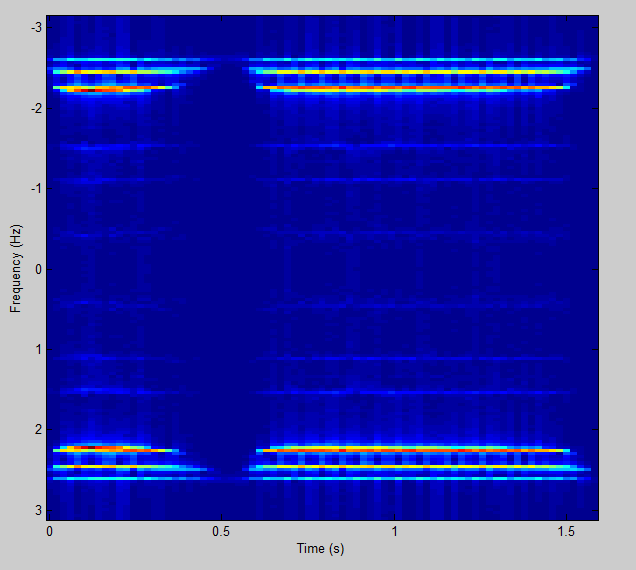
\includegraphics[scale = 0.7]{resources/labday1_report4_timefrequency.png}
\caption{Time-frequency plot.}
\label{fig:timefreq}
\end{figure}

\section*{Report 5 \& 6}

Sometimes the resolution might not be very high. 
To address this issue we consider zero padding.
This is basically augmenting a signal with zeros.
Subsequently the original samples will be interpolated.
In figure \ref{fig:zeropadding} an amplitude spectrum is shown.
The circles point to a Fourier transformed impulse response without zero padding, while the pluses indicate that zero padding has been applied.
Interpolation is obtained as every 4th sample coincides with a sample of the non augmented impulse response.

\begin{figure}[H]
    \centering
	\setlength\figureheight{6cm}
    	\setlength\figurewidth{14cm}
	% This file was created by matlab2tikz v0.4.6 running on MATLAB 8.3.
% Copyright (c) 2008--2014, Nico Schlömer <nico.schloemer@gmail.com>
% All rights reserved.
% Minimal pgfplots version: 1.3
% 
% The latest updates can be retrieved from
%   http://www.mathworks.com/matlabcentral/fileexchange/22022-matlab2tikz
% where you can also make suggestions and rate matlab2tikz.
% 
\begin{tikzpicture}

\begin{axis}[%
width=\figurewidth,
height=\figureheight,
scale only axis,
xmin=0,
xmax=1,
xlabel={Frequency (Hz)},
ymin=0,
ymax=3,
ylabel={Amplitude}
]
\addplot [color=blue,only marks,mark=o,mark options={solid},forget plot]
  table[row sep=crcr]{
0	2.7	\\
0.0769230769230769	0.849045436113243	\\
0.153846153846154	2.49555226711168	\\
0.230769230769231	0.466566034269694	\\
0.307692307692308	1.92954967807022	\\
0.384615384615385	0.321656600909142	\\
0.461538461538462	1.13447429946454	\\
0.538461538461539	1.13447429946454	\\
0.615384615384615	0.321656600909142	\\
0.692307692307692	1.92954967807022	\\
0.769230769230769	0.466566034269694	\\
0.846153846153846	2.49555226711168	\\
0.923076923076923	0.849045436113243	\\
};
\addplot [color=blue,only marks,mark=+,mark options={solid},forget plot]
  table[row sep=crcr]{
0	2.7	\\
0.0192307692307692	2.25122933360484	\\
0.0384615384615385	1.13447429946454	\\
0.0576923076923077	0.205188696869487	\\
0.0769230769230769	0.849045436113243	\\
0.0961538461538462	0.700018622361898	\\
0.115384615384615	0.321656600909142	\\
0.134615384615385	1.54961370571638	\\
0.153846153846154	2.49555226711168	\\
0.173076923076923	2.64812785369316	\\
0.192307692307692	1.92954967807022	\\
0.211538461538462	0.711304609918332	\\
0.230769230769231	0.466566034269694	\\
0.25	0.9	\\
0.269230769230769	0.466566034269694	\\
0.288461538461538	0.711304609918332	\\
0.307692307692308	1.92954967807022	\\
0.326923076923077	2.64812785369316	\\
0.346153846153846	2.49555226711168	\\
0.365384615384615	1.54961370571638	\\
0.384615384615385	0.321656600909142	\\
0.403846153846154	0.700018622361898	\\
0.423076923076923	0.849045436113243	\\
0.442307692307692	0.205188696869487	\\
0.461538461538462	1.13447429946454	\\
0.480769230769231	2.25122933360484	\\
0.5	2.7	\\
0.519230769230769	2.25122933360484	\\
0.538461538461538	1.13447429946454	\\
0.557692307692308	0.205188696869487	\\
0.576923076923077	0.849045436113243	\\
0.596153846153846	0.700018622361898	\\
0.615384615384615	0.321656600909142	\\
0.634615384615385	1.54961370571638	\\
0.653846153846154	2.49555226711168	\\
0.673076923076923	2.64812785369316	\\
0.692307692307692	1.92954967807022	\\
0.711538461538461	0.711304609918332	\\
0.730769230769231	0.466566034269694	\\
0.75	0.9	\\
0.769230769230769	0.466566034269694	\\
0.788461538461538	0.711304609918332	\\
0.807692307692308	1.92954967807022	\\
0.826923076923077	2.64812785369316	\\
0.846153846153846	2.49555226711168	\\
0.865384615384615	1.54961370571638	\\
0.884615384615385	0.321656600909142	\\
0.903846153846154	0.700018622361898	\\
0.923076923076923	0.849045436113243	\\
0.942307692307692	0.205188696869487	\\
0.961538461538461	1.13447429946454	\\
0.980769230769231	2.25122933360484	\\
};
\addplot [color=red,solid,forget plot]
  table[row sep=crcr]{
0	2.7	\\
0.0192307692307692	2.25122933360484	\\
0.0384615384615385	1.13447429946454	\\
0.0576923076923077	0.205188696869487	\\
0.0769230769230769	0.849045436113243	\\
0.0961538461538462	0.700018622361898	\\
0.115384615384615	0.321656600909142	\\
0.134615384615385	1.54961370571638	\\
0.153846153846154	2.49555226711168	\\
0.173076923076923	2.64812785369316	\\
0.192307692307692	1.92954967807022	\\
0.211538461538462	0.711304609918332	\\
0.230769230769231	0.466566034269694	\\
0.25	0.9	\\
0.269230769230769	0.466566034269694	\\
0.288461538461538	0.711304609918332	\\
0.307692307692308	1.92954967807022	\\
0.326923076923077	2.64812785369316	\\
0.346153846153846	2.49555226711168	\\
0.365384615384615	1.54961370571638	\\
0.384615384615385	0.321656600909142	\\
0.403846153846154	0.700018622361898	\\
0.423076923076923	0.849045436113243	\\
0.442307692307692	0.205188696869487	\\
0.461538461538462	1.13447429946454	\\
0.480769230769231	2.25122933360484	\\
0.5	2.7	\\
0.519230769230769	2.25122933360484	\\
0.538461538461538	1.13447429946454	\\
0.557692307692308	0.205188696869487	\\
0.576923076923077	0.849045436113243	\\
0.596153846153846	0.700018622361898	\\
0.615384615384615	0.321656600909142	\\
0.634615384615385	1.54961370571638	\\
0.653846153846154	2.49555226711168	\\
0.673076923076923	2.64812785369316	\\
0.692307692307692	1.92954967807022	\\
0.711538461538461	0.711304609918332	\\
0.730769230769231	0.466566034269694	\\
0.75	0.9	\\
0.769230769230769	0.466566034269694	\\
0.788461538461538	0.711304609918332	\\
0.807692307692308	1.92954967807022	\\
0.826923076923077	2.64812785369316	\\
0.846153846153846	2.49555226711168	\\
0.865384615384615	1.54961370571638	\\
0.884615384615385	0.321656600909142	\\
0.903846153846154	0.700018622361898	\\
0.923076923076923	0.849045436113243	\\
0.942307692307692	0.205188696869487	\\
0.961538461538461	1.13447429946454	\\
0.980769230769231	2.25122933360484	\\
};
\addplot [color=blue,only marks,mark=o,mark options={solid},forget plot]
  table[row sep=crcr]{
0	2.7	\\
0.0769230769230769	0.849045436113243	\\
0.153846153846154	2.49555226711168	\\
0.230769230769231	0.466566034269694	\\
0.307692307692308	1.92954967807022	\\
0.384615384615385	0.321656600909142	\\
0.461538461538462	1.13447429946454	\\
0.538461538461539	1.13447429946454	\\
0.615384615384615	0.321656600909142	\\
0.692307692307692	1.92954967807022	\\
0.769230769230769	0.466566034269694	\\
0.846153846153846	2.49555226711168	\\
0.923076923076923	0.849045436113243	\\
};
\addplot [color=blue,only marks,mark=+,mark options={solid},forget plot]
  table[row sep=crcr]{
0	2.7	\\
0.0192307692307692	2.25122933360484	\\
0.0384615384615385	1.13447429946454	\\
0.0576923076923077	0.205188696869487	\\
0.0769230769230769	0.849045436113243	\\
0.0961538461538462	0.700018622361898	\\
0.115384615384615	0.321656600909142	\\
0.134615384615385	1.54961370571638	\\
0.153846153846154	2.49555226711168	\\
0.173076923076923	2.64812785369316	\\
0.192307692307692	1.92954967807022	\\
0.211538461538462	0.711304609918332	\\
0.230769230769231	0.466566034269694	\\
0.25	0.9	\\
0.269230769230769	0.466566034269694	\\
0.288461538461538	0.711304609918332	\\
0.307692307692308	1.92954967807022	\\
0.326923076923077	2.64812785369316	\\
0.346153846153846	2.49555226711168	\\
0.365384615384615	1.54961370571638	\\
0.384615384615385	0.321656600909142	\\
0.403846153846154	0.700018622361898	\\
0.423076923076923	0.849045436113243	\\
0.442307692307692	0.205188696869487	\\
0.461538461538462	1.13447429946454	\\
0.480769230769231	2.25122933360484	\\
0.5	2.7	\\
0.519230769230769	2.25122933360484	\\
0.538461538461538	1.13447429946454	\\
0.557692307692308	0.205188696869487	\\
0.576923076923077	0.849045436113243	\\
0.596153846153846	0.700018622361898	\\
0.615384615384615	0.321656600909142	\\
0.634615384615385	1.54961370571638	\\
0.653846153846154	2.49555226711168	\\
0.673076923076923	2.64812785369316	\\
0.692307692307692	1.92954967807022	\\
0.711538461538461	0.711304609918332	\\
0.730769230769231	0.466566034269694	\\
0.75	0.9	\\
0.769230769230769	0.466566034269694	\\
0.788461538461538	0.711304609918332	\\
0.807692307692308	1.92954967807022	\\
0.826923076923077	2.64812785369316	\\
0.846153846153846	2.49555226711168	\\
0.865384615384615	1.54961370571638	\\
0.884615384615385	0.321656600909142	\\
0.903846153846154	0.700018622361898	\\
0.923076923076923	0.849045436113243	\\
0.942307692307692	0.205188696869487	\\
0.961538461538461	1.13447429946454	\\
0.980769230769231	2.25122933360484	\\
};
\addplot [color=red,solid,forget plot]
  table[row sep=crcr]{
0	2.7	\\
0.0192307692307692	2.25122933360484	\\
0.0384615384615385	1.13447429946454	\\
0.0576923076923077	0.205188696869487	\\
0.0769230769230769	0.849045436113243	\\
0.0961538461538462	0.700018622361898	\\
0.115384615384615	0.321656600909142	\\
0.134615384615385	1.54961370571638	\\
0.153846153846154	2.49555226711168	\\
0.173076923076923	2.64812785369316	\\
0.192307692307692	1.92954967807022	\\
0.211538461538462	0.711304609918332	\\
0.230769230769231	0.466566034269694	\\
0.25	0.9	\\
0.269230769230769	0.466566034269694	\\
0.288461538461538	0.711304609918332	\\
0.307692307692308	1.92954967807022	\\
0.326923076923077	2.64812785369316	\\
0.346153846153846	2.49555226711168	\\
0.365384615384615	1.54961370571638	\\
0.384615384615385	0.321656600909142	\\
0.403846153846154	0.700018622361898	\\
0.423076923076923	0.849045436113243	\\
0.442307692307692	0.205188696869487	\\
0.461538461538462	1.13447429946454	\\
0.480769230769231	2.25122933360484	\\
0.5	2.7	\\
0.519230769230769	2.25122933360484	\\
0.538461538461538	1.13447429946454	\\
0.557692307692308	0.205188696869487	\\
0.576923076923077	0.849045436113243	\\
0.596153846153846	0.700018622361898	\\
0.615384615384615	0.321656600909142	\\
0.634615384615385	1.54961370571638	\\
0.653846153846154	2.49555226711168	\\
0.673076923076923	2.64812785369316	\\
0.692307692307692	1.92954967807022	\\
0.711538461538461	0.711304609918332	\\
0.730769230769231	0.466566034269694	\\
0.75	0.9	\\
0.769230769230769	0.466566034269694	\\
0.788461538461538	0.711304609918332	\\
0.807692307692308	1.92954967807022	\\
0.826923076923077	2.64812785369316	\\
0.846153846153846	2.49555226711168	\\
0.865384615384615	1.54961370571638	\\
0.884615384615385	0.321656600909142	\\
0.903846153846154	0.700018622361898	\\
0.923076923076923	0.849045436113243	\\
0.942307692307692	0.205188696869487	\\
0.961538461538461	1.13447429946454	\\
0.980769230769231	2.25122933360484	\\
};
\end{axis}
\end{tikzpicture}%
	\caption{The circles indicate no zero padding while the pluses do.}
	\label{fig:zeropadding}
\end{figure}

\section*{Report 7}
To demonstrate the convolution property, as noted in equation \ref{eq:convolution}, $X(\omega)H(\omega)$ should be identical to $Y(\omega)$.
\begin{equation}
y[n] = x[n] * h[n] \Leftrightarrow Y(\omega) = X(\omega)H(\omega)
\label{eq:convolution}
\end{equation}
For this reason we convolute the vectors x and h to get an y. 
Afterwards we apply the Fourier transform on y.
Parallel to this x and h are Fourier transformed after which they are multiplied.
This should result in identical plots.
For the latter case x and h should have the length of y.
To obtain the right length we make use of zero padding.
In figure \ref{fig:convolution} the two plots are identical and thus the convolution property is demonstrated.

\begin{figure}[H]
    \centering
	\setlength\figureheight{6cm}
    	\setlength\figurewidth{14cm}
	% This file was created by matlab2tikz v0.4.6 running on MATLAB 8.3.
% Copyright (c) 2008--2014, Nico Schlömer <nico.schloemer@gmail.com>
% All rights reserved.
% Minimal pgfplots version: 1.3
% 
% The latest updates can be retrieved from
%   http://www.mathworks.com/matlabcentral/fileexchange/22022-matlab2tikz
% where you can also make suggestions and rate matlab2tikz.
% 
\begin{tikzpicture}

\begin{axis}[%
width=\figurewidth,
height=\figureheight,
scale only axis,
xmin=-3.14159265358979,
xmax=3.14114301960474,
ymin=0,
ymax=2500,
name=plot1
]
\addplot [color=blue,solid,forget plot]
  table[row sep=crcr]{
-3.14159265358979	19.8926584456553	\\
-3.12675473208293	0.0532087870446882	\\
-3.11911095433697	2.57064553821331	\\
-3.11101754260595	1.27544115516442	\\
-3.10517230080022	0.012485403205535	\\
-3.08943511132324	1.91644737522381	\\
-3.08538840545773	0.212474242094612	\\
-3.08314023553245	0.0838492963971151	\\
-3.07234901989109	2.49722134003265	\\
-3.06830231402558	0.0962186821635277	\\
-3.05706146439917	1.72924839592516	\\
-3.0485184186831	1.66281160520585	\\
-3.04627024875781	0.127820081329008	\\
-3.03098269326589	0.0706835516622831	\\
-3.02603671943027	1.86093549827026	\\
-3.02333891551993	0.161773970788943	\\
-3.02154037957971	1.38923085606008	\\
-3.00355502017745	3.01650899809105	\\
-3.00040758228205	0.216074057948433	\\
-2.99141490258092	0.0367743314174455	\\
-2.98197258889473	1.77238192397133	\\
-2.97972441896945	2.41393860297375	\\
-2.97118137325338	0.0928657729370627	\\
-2.95724271971663	2.0902597787146	\\
-2.95364564783617	0.0282881474970191	\\
-2.9451026021201	0.117811171829853	\\
-2.94060626226954	1.60211367575097	\\
-2.93655955640403	0.0333338621943806	\\
-2.92711724271784	5.25965848044103	\\
-2.92396980482245	4.23078513885601	\\
-2.91587639309143	0.118069256589241	\\
-2.90823261534547	0.124401303364409	\\
-2.90598444542018	4.3862467870769	\\
-2.88889835398804	3.58747122572868	\\
-2.88530128210759	0.150608405431404	\\
-2.88080494225702	1.49326518519667	\\
-2.87540933443634	0.0252196185317378	\\
-2.8655173867651	2.27296335694572	\\
-2.86147068089959	0.12693446657177	\\
-2.84933056330307	2.56642618414948	\\
-2.83898898164677	0.0643457918178676	\\
-2.83089556991575	0.128446439925093	\\
-2.82639923006518	2.21339228450317	\\
-2.82145325622956	0.107161458215456	\\
-2.81875545231922	3.61938596000812	\\
-2.80166936088708	0.0188790899191806	\\
-2.79582411908134	2.90312861041924	\\
-2.79402558314112	0.210704076393256	\\
-2.78098619757448	3.05206849108307	\\
-2.77514095576874	3.14897397933414	\\
-2.77019498193312	0.00153586525415124	\\
-2.76030303426188	0.190128689478314	\\
-2.7517599885458	2.03384603580528	\\
-2.74681401471018	0.0771736221028695	\\
-2.74366657681479	2.01446283056626	\\
-2.73287536117343	2.32433014135083	\\
-2.72478194944241	0.0940196992389875	\\
-2.71533963575623	0.145533812642321	\\
-2.71084329590566	2.72575122386714	\\
-2.70544768808498	2.42779957625067	\\
-2.70274988417465	0.0734579525711054	\\
-2.68521415875744	0.0462058253577377	\\
-2.6825163548471	4.05199063103163	\\
-2.67622147905631	3.35656895436007	\\
-2.66857770131035	0.144612236845544	\\
-2.65958502160922	3.46435485198692	\\
-2.64969307393798	0.0360835363255782	\\
-2.64924343995292	0.42984603117975	\\
-2.63485515243111	8.82579083502318	\\
-2.62721137468515	0.564476074568702	\\
-2.62001723092425	49.9399519297817	\\
-2.60967564926795	5.04787971905156	\\
-2.60652821137255	241.563377121866	\\
-2.60158223753693	410.306944561965	\\
-2.59348882580592	2.39071400449906	\\
-2.59034138791052	13.1669073905317	\\
-2.57685236835882	0.284559849196704	\\
-2.57595310038871	0.149368125229052	\\
-2.57370493046343	7.28455897645908	\\
-2.56066554489679	5.33033992568238	\\
-2.55392103512094	0.230489414552615	\\
-2.54492835541981	6.44038442499614	\\
-2.54043201556925	0.33703182457791	\\
-2.53098970188306	0.189490523276336	\\
-2.52199702218193	8.72813803699814	\\
-2.51795031631642	0.304868032518704	\\
-2.50491093074978	21.1624892630286	\\
-2.49636788503371	27.9830091157402	\\
-2.49591825104865	0.727890114091731	\\
-2.48467740142224	3.76176580377005	\\
-2.47658398969122	165.53867903062	\\
-2.47208764984066	19.8929677550075	\\
-2.4644438720947	492.986662568109	\\
-2.45949789825908	585.133990276727	\\
-2.44825704863266	0.432385168545974	\\
-2.43926436893153	0.454501772797956	\\
-2.4365665650212	15.9468842395576	\\
-2.42847315329018	15.979168879326	\\
-2.42577534937984	0.137044810441969	\\
-2.41003815990286	0.223978183776946	\\
-2.40644108802241	16.5498674043315	\\
-2.40284401614196	0.519622744440768	\\
-2.39025426456038	9.74483230277733	\\
-2.38350975478453	12.8167756750116	\\
-2.38036231688913	0.559236167527878	\\
-2.37092000320295	0.430379161123992	\\
-2.36147768951676	7.59222635706518	\\
-2.35698134966619	0.108118890436206	\\
-2.35428354575585	9.93512366979884	\\
-2.33854635627888	11.4656761149616	\\
-2.33180184650303	1.0287496436849	\\
-2.32820477462258	0.338504212020415	\\
-2.32056099687662	16.7183720096503	\\
-2.31471575507088	23.5207211339421	\\
-2.3052734413847	1.44956711035969	\\
-2.29223405581806	54.8185618571025	\\
-2.28818734995255	1.61102489167945	\\
-2.27964430423648	4.23862174118417	\\
-2.2742486964158	106.167950884941	\\
-2.26885308859512	182.22370137463	\\
-2.25851150693882	6.06144052992204	\\
-2.24502248738712	2476.13546958913	\\
-2.24367358543195	1013.98945314128	\\
-2.23243273580554	6.83375636334474	\\
-2.22883566392509	52.0515388884008	\\
-2.21894371625385	1.39709458450789	\\
-2.20725323264238	20.2476741076976	\\
-2.20320652677687	1.15512796207575	\\
-2.20005908888147	15.6909148150422	\\
-2.18657006932978	0.403730777514918	\\
-2.17532921970337	27.6473672346279	\\
-2.17263141579303	0.720286869288151	\\
-2.16633654000224	0.734390437905012	\\
-2.15914239624133	18.5528372629984	\\
-2.15374678842065	13.8916730146768	\\
-2.1501497165402	0.653642562814454	\\
-2.14070740285402	0.169766100504169	\\
-2.13755996495862	12.7697069806375	\\
-2.11732643563108	0.549272029838374	\\
-2.11597753367591	5.89962358806633	\\
-2.10788412194489	13.7634577359606	\\
-2.10338778209433	0.349053686772005	\\
-2.0943951023932	0.210274044405798	\\
-2.08989876254263	7.94066866383391	\\
-2.0840535207369	8.14342146687816	\\
-2.07191340314037	0.197401818828818	\\
-2.06157182148407	26.1718804663576	\\
-2.05842438358868	0.773915104326615	\\
-2.05527694569328	8.79359719167923	\\
-2.04853243591743	0.189862054928003	\\
-2.03504341636574	0.237143504436913	\\
-2.0323456124554	4.99066752537407	\\
-2.0220040307991	0.0956697335516264	\\
-2.02110476282899	4.92125576897894	\\
-2.00266976944167	0.0774503957368301	\\
-1.99952233154627	7.45371945192958	\\
-1.99772379560605	4.6006647382492	\\
-1.98918074988997	0.12749680707944	\\
-1.97973843620379	0.146787854193875	\\
-1.96939685454749	6.35453068734138	\\
-1.96849758657737	4.20319594474824	\\
-1.96265234477164	0.0807702240775046	\\
-1.94736478927972	3.74503331278603	\\
-1.94331808341421	0.0761937905147443	\\
-1.93342613574297	0.0302204524480887	\\
-1.92982906386252	4.2749282586906	\\
-1.92398382205678	5.68451894520705	\\
-1.92038675017633	0.283028327672143	\\
-1.91049480250509	0.123428201161085	\\
-1.90734736460969	4.54386895558947	\\
-1.8875634692672	0.102016699557211	\\
-1.88396639738675	4.48080262933705	\\
-1.87947005753619	4.35571560129846	\\
-1.87407444971551	0.178555934936627	\\
-1.86463213602932	0.0685195298608476	\\
-1.85384092038797	3.92418099057164	\\
-1.84170080279144	0.0268939699058458	\\
-1.83945263286616	4.62584030444586	\\
-1.83855336489604	4.15839707868827	\\
-1.8286614172248	0.074279113519074	\\
-1.81876946955356	0.0750306472233845	\\
-1.80977678985243	4.07065149183564	\\
-1.80842788789726	3.48512804005471	\\
-1.79583813631568	0.0427814343622637	\\
-1.78954326052489	0.365363633867683	\\
-1.78504692067432	16.016713380486	\\
-1.77830241089847	7.11393971060506	\\
-1.7729068030778	0.278726905174866	\\
-1.76211558743644	3.68904740694711	\\
-1.7594177835261	0.0746234355896293	\\
-1.74592876397441	5.00468214258017	\\
-1.74323096006407	0.16296470437005	\\
-1.73648645028822	0.0468474515857732	\\
-1.72254779675147	2.88233537524637	\\
-1.7180514569009	5.54455975910776	\\
-1.71400475103539	0.141959094005153	\\
-1.70366316937909	0.0554711875012217	\\
-1.70006609749864	4.71499163350529	\\
-1.69287195373774	3.39774808833229	\\
-1.68073183614121	0.082190368128078	\\
-1.67578586230559	6.35359175314588	\\
-1.66769245057457	0.190171800012267	\\
-1.65780050290333	0.0709065378871592	\\
-1.6560019669631	8.9570059818486	\\
-1.64745892124703	12.9226088121107	\\
-1.64476111733669	0.28725170218465	\\
-1.63486916966545	0.0209794613833366	\\
-1.63217136575511	8.41082156820344	\\
-1.61193783642757	0.0977324817758621	\\
-1.60879039853217	14.032888311883	\\
-1.60654222860689	10.6541498279629	\\
-1.59844881687587	0.286813108722075	\\
-1.58900650318968	0.293239032341302	\\
-1.58630869927935	21.7217540403053	\\
-1.57596711762305	0.0654171936989979	\\
-1.56382700002652	18.4826848804303	\\
-1.5588810261909	0.700755695098959	\\
-1.55528395431045	25.3010275374739	\\
-1.54808981054954	1.06558784718216	\\
-1.53864749686336	40.4197337709948	\\
-1.53010445114728	0.660976059794117	\\
-1.52246067340132	111.4625235256	\\
-1.51166945775997	91.1529537651241	\\
-1.50672348392434	0.235685205812729	\\
-1.49952934016344	25.8384254852915	\\
-1.49638190226805	0.282315541283869	\\
-1.48693958858186	24.3182308636348	\\
-1.48379215068646	0.644918188313327	\\
-1.47434983700028	0.660724444002167	\\
-1.47030313113477	12.1584709253588	\\
-1.45096886977734	0.149429691982144	\\
-1.44782143188194	6.27675810845753	\\
-1.44602289594172	8.78460013554648	\\
-1.43703021624059	0.271748147190503	\\
-1.42803753653946	0.220751682035347	\\
-1.424440464659	7.71063611254086	\\
-1.41859522285327	7.47958593051218	\\
-1.41499815097282	0.180020898684117	\\
-1.40285803337629	10.2314632616844	\\
-1.40150913142112	0.118701543739853	\\
-1.38127560209358	0.238693595014367	\\
-1.38037633412347	10.7037387112309	\\
-1.36913548449705	0.0188655951495292	\\
-1.36104207276604	9.1028081624014	\\
-1.35924353682581	0.403148375165112	\\
-1.34755305321434	28.0905820761561	\\
-1.34440561531895	0.57527786401742	\\
-1.33316476569253	16.2832434531534	\\
-1.33181586373736	10.7515234651398	\\
-1.32282318403623	0.0546328682440252	\\
-1.31338087035005	0.0942097225965186	\\
-1.30303928869375	8.9321424859863	\\
-1.28999990312711	0.0735324312574333	\\
-1.28775173320183	5.84009946538904	\\
-1.28370502733632	0.117807301005373	\\
-1.27066564176968	0.0972705818588063	\\
-1.26482039996395	6.23505810243354	\\
-1.25942479214327	4.10387246584359	\\
-1.25402918432259	0.0355173616024903	\\
-1.24503650462146	0.249650943925795	\\
-1.24009053078584	4.35538475815771	\\
-1.22120590341346	0.182006403034195	\\
-1.21760883153301	7.24358599396274	\\
-1.21176358972728	5.82064118678822	\\
-1.20681761589166	0.226991257713179	\\
-1.19827457017558	0.539531648837398	\\
-1.19467749829513	10.228883933073	\\
-1.1784906748331	7.06030676064892	\\
-1.17624250490781	0.156336414770753	\\
-1.1650016552814	8.71934224821784	\\
-1.16230385137106	0.208430751324701	\\
-1.15286153768488	0.255527236054257	\\
-1.14971409978948	15.5596527030979	\\
-1.14207032204352	12.5816725721892	\\
-1.13892288414812	0.222072667434679	\\
-1.12408496264126	31.8124416056185	\\
-1.12183679271598	0.437660871933631	\\
-1.10744850519417	1.63740204294597	\\
-1.10250253135855	240.523702212192	\\
-1.09665728955281	52.8705447260934	\\
-1.08586607391146	1.72584526169728	\\
-1.08451717195629	0.651574085317387	\\
-1.07372595631493	19.0603023354286	\\
-1.07012888443448	0.255184262823433	\\
-1.05798876683795	9.25825358128747	\\
-1.05484132894256	0.598948654264419	\\
-1.05124425706211	9.49877816333689	\\
-1.03101072773456	0.208939010776117	\\
-1.02831292382422	12.3179050320662	\\
-1.01797134216792	5.44305892729178	\\
-1.01482390427253	0.459515040520143	\\
-1.01032756442196	17.1172038797662	\\
-1.00088525073578	0.259124489500461	\\
-0.996838544870269	0.291999842737283	\\
-0.987845865169139	11.802405515419	\\
-0.983349525318574	5.81562217527288	\\
-0.97750428351284	0.130358097585567	\\
-0.968061969826653	0.082340108109789	\\
-0.963115995991032	5.84366157089055	\\
-0.955022584260015	0.0702963892319461	\\
-0.941083930723263	5.11028380092381	\\
-0.932540885007189	0.108803297400991	\\
-0.922648937335946	0.370608775198911	\\
-0.919051865455494	6.0074553421597	\\
-0.905113211918743	0.10698723546407	\\
-0.897469434172782	6.3642154214645	\\
-0.88622858454637	0.218420546540637	\\
-0.876786270860183	0.249054060468997	\\
-0.873638832964788	6.39969945840234	\\
-0.863297251308488	0.247563216350043	\\
-0.856103107547584	6.45955227983675	\\
-0.850257865741849	6.49052127704355	\\
-0.840365918070606	0.214449183592143	\\
-0.830923604384419	0.309826053382562	\\
-0.828675434459137	6.54115990189622	\\
-0.820132388743063	2.62955605789736	\\
-0.813387878967216	0.0355907240214964	\\
-0.808441905131594	0.0670105912474191	\\
-0.805744101221255	4.93293718019949	\\
-0.7846113039236	0.0365951810973887	\\
-0.78191350001326	4.30432597361454	\\
-0.775618624222469	5.52893272832956	\\
-0.772021552342018	0.436938417722433	\\
-0.764377774596057	4.25188963121735	\\
-0.753586558954701	0.153758612803091	\\
-0.743694611283458	0.226560192844928	\\
-0.741896075343232	3.65355650402903	\\
-0.728856689776593	5.50186116376013	\\
-0.725259617896141	0.430002820634587	\\
-0.715817304209954	0.110207185854368	\\
-0.714018768269729	5.64307291122997	\\
-0.706374990523768	7.17083238821062	\\
-0.703227552628372	0.226992840528917	\\
-0.689738533076677	0.0781777717468108	\\
-0.689288899091621	6.09191027381145	\\
-0.678048049465208	0.199236321363024	\\
-0.665907931868682	6.71049915763951	\\
-0.662310859988231	0.344252916824491	\\
-0.659613056077891	6.72434110868123	\\
-0.647023304496309	0.361076953307015	\\
-0.638030624795179	5.62343067291799	\\
-0.636232088854953	5.12361480545967	\\
-0.633084650959558	0.209131575006773	\\
-0.620045265392919	8.02122986699579	\\
-0.610602951706733	0.475146655222324	\\
-0.601160638020546	0.436265881703127	\\
-0.597113932155037	8.09618061069338	\\
-0.591718324334359	9.43462213356189	\\
-0.580477474707947	0.157104023421555	\\
-0.573283330947043	8.93914002740303	\\
-0.564740285230969	0.152139142849741	\\
-0.550351997709161	8.07508192323586	\\
-0.545406023873539	8.65280691066647	\\
-0.541808951993088	0.584091572937608	\\
-0.527870298456336	14.0700639340484	\\
-0.524273226575884	0.178777674974315	\\
-0.514830912889697	0.731631390134797	\\
-0.507187135143737	7.39062775239001	\\
-0.499992991382832	16.4936521005183	\\
-0.495946285517324	1.11473101140068	\\
-0.486503971831137	1.32448791015046	\\
-0.482457265965629	23.3986449873541	\\
-0.475712756189781	27.6795569756248	\\
-0.474813488219668	0.475744951951137	\\
-0.462673370623143	2.0960773391043	\\
-0.4527814229519	51.7867280080287	\\
-0.444688011220883	1.05865098700483	\\
-0.437943501445035	42.0928838079822	\\
-0.430749357684131	36.9311768297169	\\
-0.426702651818622	0.515291527572411	\\
-0.41411290023704	33.5573356924844	\\
-0.410515828356588	0.395447548758222	\\
-0.403771318580741	1.29667402693208	\\
-0.391181566999159	15.8290642070355	\\
-0.389832665043989	27.6274800231544	\\
-0.377242913462407	1.28736203229961	\\
-0.375444377522181	20.1649259779998	\\
-0.371397671656672	2.33262879157686	\\
-0.361505723985429	14.8191930587707	\\
-0.348016704433734	0.604342762466176	\\
-0.341272194657887	0.477171926523295	\\
-0.338124756762491	13.7181008208293	\\
-0.323736469240683	0.0634528301774847	\\
-0.322387567285514	9.47287770413512	\\
-0.316542325479779	8.79131361261518	\\
-0.312045985629214	0.611935683659901	\\
-0.302154037957971	0.230086716936798	\\
-0.297657698107406	10.0858880685462	\\
-0.278773070735033	0.601671674176026	\\
-0.276974534794807	10.3801846251015	\\
-0.274276730884468	11.4759256230187	\\
-0.271129292989072	0.720670297543253	\\
-0.253143933586812	13.0511753102932	\\
-0.252244665616699	0.272894872887547	\\
-0.236957110124778	0.0688344029671348	\\
-0.236057842154665	5.08395985277606	\\
-0.229762966363874	7.29623724844187	\\
-0.220320652677687	0.138001054348589	\\
-0.206381999140935	6.40210038923912	\\
-0.20323456124554	0.172517564857273	\\
-0.197838953424862	0.294857014891671	\\
-0.189745541693845	3.9799361479004	\\
-0.187047737783506	0.0637000187503415	\\
-0.183450665903054	6.19420820545885	\\
-0.169961646351358	0.205181356843812	\\
-0.161868234620342	4.23956348029029	\\
-0.152875554919211	2.82161838287159	\\
-0.151976286949099	0.192417664670228	\\
-0.142084339277855	0.0282934343198709	\\
-0.138037633412347	5.39676833979871	\\
-0.129494587696273	2.50760534042733	\\
-0.127696051756047	0.0933586920275544	\\
-0.115106300174465	2.72517227484558	\\
-0.105663986488278	0.0714281588344531	\\
-0.0984698427273747	0.128850734872603	\\
-0.0926246009216398	2.7695015485174	\\
-0.0777866794147752	0.187643878288714	\\
-0.0755385094894927	2.97654141208107	\\
-0.0683443657285889	1.73845254928587	\\
-0.0660961958033064	0.0194202524749926	\\
-0.0553049801619503	0.0427546446086761	\\
-0.051707908281498	2.28863913103362	\\
-0.043614496550481	1.26335580136522	\\
-0.0422655945953117	0.132332292338383	\\
-0.0215824312827122	0.216440371596831	\\
-0.0170860914321471	3.21492506903341	\\
-0.00449633985056508	0.0778995026941969	\\
-4.44089209850063e-16	5.09414969888162	\\
0.00449633985056463	0.0778995026941969	\\
0.0170860914321467	3.21492506903341	\\
0.0215824312827118	0.216440371596831	\\
0.0422655945953108	0.132332292338383	\\
0.0436144965504806	1.26335580136522	\\
0.0517079082814975	2.28863913103362	\\
0.0553049801619494	0.0427546446086761	\\
0.0660961958033055	0.0194202524749926	\\
0.068344365728588	1.73845254928587	\\
0.0755385094894923	2.97654141208107	\\
0.0777866794147748	0.187643878288714	\\
0.0926246009216394	2.7695015485174	\\
0.0984698427273738	0.128850734872603	\\
0.105663986488278	0.0714281588344531	\\
0.115106300174465	2.72517227484558	\\
0.127696051756047	0.0933586920275544	\\
0.129494587696273	2.50760534042733	\\
0.138037633412346	5.39676833979871	\\
0.142084339277855	0.0282934343198709	\\
0.151976286949098	0.192417664670228	\\
0.152875554919211	2.82161838287159	\\
0.161868234620341	4.23956348029029	\\
0.169961646351358	0.205181356843812	\\
0.183450665903053	6.19420820545885	\\
0.187047737783505	0.0637000187503415	\\
0.189745541693844	3.9799361479004	\\
0.197838953424861	0.294857014891671	\\
0.20323456124554	0.172517564857273	\\
0.206381999140935	6.40210038923912	\\
0.220320652677687	0.138001054348589	\\
0.229762966363873	7.29623724844187	\\
0.236057842154664	5.08395985277606	\\
0.236957110124777	0.0688344029671348	\\
0.252244665616698	0.272894872887547	\\
0.253143933586812	13.0511753102932	\\
0.271129292989071	0.720670297543253	\\
0.274276730884467	11.4759256230187	\\
0.276974534794806	10.3801846251015	\\
0.278773070735032	0.601671674176026	\\
0.297657698107405	10.0858880685462	\\
0.30215403795797	0.230086716936798	\\
0.312045985629213	0.611935683659901	\\
0.316542325479778	8.79131361261518	\\
0.322387567285513	9.47287770413512	\\
0.323736469240683	0.0634528301774847	\\
0.338124756762491	13.7181008208293	\\
0.341272194657886	0.477171926523295	\\
0.348016704433733	0.604342762466176	\\
0.361505723985429	14.8191930587707	\\
0.371397671656672	2.33262879157686	\\
0.375444377522181	20.1649259779998	\\
0.377242913462406	1.28736203229961	\\
0.389832665043989	27.6274800231544	\\
0.391181566999158	15.8290642070355	\\
0.40377131858074	1.29667402693208	\\
0.410515828356588	0.395447548758222	\\
0.41411290023704	33.5573356924844	\\
0.426702651818622	0.515291527572411	\\
0.43074935768413	36.9311768297169	\\
0.437943501445035	42.0928838079822	\\
0.444688011220882	1.05865098700483	\\
0.452781422951899	51.7867280080287	\\
0.462673370623142	2.0960773391043	\\
0.474813488219668	0.475744951951137	\\
0.475712756189781	27.6795569756248	\\
0.482457265965628	23.3986449873541	\\
0.486503971831137	1.32448791015046	\\
0.495946285517324	1.11473101140068	\\
0.499992991382832	16.4936521005183	\\
0.507187135143736	7.39062775239001	\\
0.514830912889697	0.731631390134797	\\
0.524273226575883	0.178777674974315	\\
0.527870298456335	14.0700639340484	\\
0.541808951993087	0.584091572937608	\\
0.545406023873539	8.65280691066647	\\
0.55035199770916	8.07508192323586	\\
0.564740285230969	0.152139142849741	\\
0.573283330947042	8.93914002740303	\\
0.580477474707946	0.157104023421555	\\
0.591718324334359	9.43462213356189	\\
0.597113932155037	8.09618061069338	\\
0.601160638020545	0.436265881703127	\\
0.610602951706732	0.475146655222324	\\
0.620045265392918	8.02122986699579	\\
0.633084650959557	0.209131575006773	\\
0.636232088854953	5.12361480545967	\\
0.638030624795179	5.62343067291799	\\
0.647023304496309	0.361076953307015	\\
0.659613056077891	6.72434110868123	\\
0.66231085998823	0.344252916824491	\\
0.665907931868682	6.71049915763951	\\
0.678048049465207	0.199236321363024	\\
0.68928889909162	6.09191027381145	\\
0.689738533076677	0.0781777717468108	\\
0.703227552628372	0.226992840528917	\\
0.706374990523767	7.17083238821062	\\
0.714018768269728	5.64307291122997	\\
0.715817304209954	0.110207185854368	\\
0.72525961789614	0.430002820634587	\\
0.728856689776593	5.50186116376013	\\
0.741896075343231	3.65355650402903	\\
0.743694611283457	0.226560192844928	\\
0.7535865589547	0.153758612803091	\\
0.764377774596056	4.25188963121735	\\
0.772021552342017	0.436938417722433	\\
0.775618624222469	5.52893272832956	\\
0.78191350001326	4.30432597361454	\\
0.784611303923599	0.0365951810973887	\\
0.805744101221255	4.93293718019949	\\
0.808441905131594	0.0670105912474191	\\
0.813387878967215	0.0355907240214964	\\
0.820132388743063	2.62955605789736	\\
0.828675434459136	6.54115990189622	\\
0.830923604384419	0.309826053382562	\\
0.840365918070606	0.214449183592143	\\
0.850257865741848	6.49052127704355	\\
0.856103107547583	6.45955227983675	\\
0.863297251308487	0.247563216350043	\\
0.873638832964787	6.39969945840234	\\
0.876786270860182	0.249054060468997	\\
0.886228584546369	0.218420546540637	\\
0.897469434172781	6.3642154214645	\\
0.905113211918742	0.10698723546407	\\
0.919051865455494	6.0074553421597	\\
0.922648937335946	0.370608775198911	\\
0.932540885007189	0.108803297400991	\\
0.941083930723263	5.11028380092381	\\
0.955022584260014	0.0702963892319461	\\
0.963115995991031	5.84366157089055	\\
0.968061969826652	0.082340108109789	\\
0.97750428351284	0.130358097585567	\\
0.983349525318573	5.81562217527288	\\
0.987845865169138	11.802405515419	\\
0.996838544870268	0.291999842737283	\\
1.00088525073578	0.259124489500461	\\
1.01032756442196	17.1172038797662	\\
1.01482390427253	0.459515040520143	\\
1.01797134216792	5.44305892729178	\\
1.02831292382422	12.3179050320662	\\
1.03101072773456	0.208939010776117	\\
1.05124425706211	9.49877816333689	\\
1.05484132894256	0.598948654264419	\\
1.05798876683795	9.25825358128747	\\
1.07012888443448	0.255184262823433	\\
1.07372595631493	19.0603023354286	\\
1.08451717195629	0.651574085317387	\\
1.08586607391146	1.72584526169728	\\
1.09665728955281	52.8705447260934	\\
1.10250253135855	240.523702212192	\\
1.10744850519417	1.63740204294597	\\
1.12183679271598	0.437660871933631	\\
1.12408496264126	31.8124416056185	\\
1.13892288414812	0.222072667434679	\\
1.14207032204352	12.5816725721892	\\
1.14971409978948	15.5596527030979	\\
1.15286153768488	0.255527236054257	\\
1.16230385137106	0.208430751324701	\\
1.1650016552814	8.71934224821784	\\
1.17624250490781	0.156336414770753	\\
1.1784906748331	7.06030676064892	\\
1.19467749829513	10.228883933073	\\
1.19827457017558	0.539531648837398	\\
1.20681761589166	0.226991257713179	\\
1.21176358972728	5.82064118678822	\\
1.21760883153301	7.24358599396274	\\
1.22120590341346	0.182006403034195	\\
1.24009053078584	4.35538475815771	\\
1.24503650462146	0.249650943925795	\\
1.25402918432259	0.0355173616024903	\\
1.25942479214327	4.10387246584359	\\
1.26482039996394	6.23505810243354	\\
1.27066564176968	0.0972705818588063	\\
1.28370502733632	0.117807301005373	\\
1.28775173320183	5.84009946538904	\\
1.28999990312711	0.0735324312574333	\\
1.30303928869375	8.9321424859863	\\
1.31338087035005	0.0942097225965186	\\
1.32282318403623	0.0546328682440252	\\
1.33181586373736	10.7515234651398	\\
1.33316476569253	16.2832434531534	\\
1.34440561531895	0.57527786401742	\\
1.34755305321434	28.0905820761561	\\
1.35924353682581	0.403148375165112	\\
1.36104207276604	9.1028081624014	\\
1.36913548449705	0.0188655951495292	\\
1.38037633412347	10.7037387112309	\\
1.38127560209358	0.238693595014367	\\
1.40150913142112	0.118701543739853	\\
1.40285803337629	10.2314632616844	\\
1.41499815097282	0.180020898684117	\\
1.41859522285327	7.47958593051218	\\
1.424440464659	7.71063611254086	\\
1.42803753653946	0.220751682035347	\\
1.43703021624059	0.271748147190503	\\
1.44602289594172	8.78460013554648	\\
1.44782143188194	6.27675810845753	\\
1.45096886977734	0.149429691982144	\\
1.47030313113477	12.1584709253588	\\
1.47434983700028	0.660724444002167	\\
1.48379215068646	0.644918188313327	\\
1.48693958858186	24.3182308636348	\\
1.49638190226804	0.282315541283869	\\
1.49952934016344	25.8384254852915	\\
1.50672348392434	0.235685205812729	\\
1.51166945775997	91.1529537651241	\\
1.52246067340132	111.4625235256	\\
1.53010445114728	0.660976059794117	\\
1.53864749686336	40.4197337709948	\\
1.54808981054954	1.06558784718216	\\
1.55528395431045	25.3010275374739	\\
1.5588810261909	0.700755695098959	\\
1.56382700002652	18.4826848804303	\\
1.57596711762305	0.0654171936989979	\\
1.58630869927935	21.7217540403053	\\
1.58900650318968	0.293239032341302	\\
1.59844881687587	0.286813108722075	\\
1.60654222860689	10.6541498279629	\\
1.60879039853217	14.032888311883	\\
1.61193783642757	0.0977324817758621	\\
1.63217136575511	8.41082156820344	\\
1.63486916966545	0.0209794613833366	\\
1.64476111733669	0.28725170218465	\\
1.64745892124703	12.9226088121107	\\
1.6560019669631	8.9570059818486	\\
1.65780050290333	0.0709065378871592	\\
1.66769245057457	0.190171800012267	\\
1.67578586230559	6.35359175314588	\\
1.68073183614121	0.082190368128078	\\
1.69287195373774	3.39774808833229	\\
1.70006609749864	4.71499163350529	\\
1.70366316937909	0.0554711875012217	\\
1.71400475103539	0.141959094005153	\\
1.7180514569009	5.54455975910776	\\
1.72254779675147	2.88233537524637	\\
1.73648645028822	0.0468474515857732	\\
1.74323096006407	0.16296470437005	\\
1.7459287639744	5.00468214258017	\\
1.7594177835261	0.0746234355896293	\\
1.76211558743644	3.68904740694711	\\
1.77290680307779	0.278726905174866	\\
1.77830241089847	7.11393971060506	\\
1.78504692067432	16.016713380486	\\
1.78954326052489	0.365363633867683	\\
1.79583813631568	0.0427814343622637	\\
1.80842788789726	3.48512804005471	\\
1.80977678985243	4.07065149183564	\\
1.81876946955356	0.0750306472233845	\\
1.8286614172248	0.074279113519074	\\
1.83855336489604	4.15839707868827	\\
1.83945263286616	4.62584030444586	\\
1.84170080279144	0.0268939699058458	\\
1.85384092038796	3.92418099057164	\\
1.86463213602932	0.0685195298608476	\\
1.87407444971551	0.178555934936627	\\
1.87947005753619	4.35571560129846	\\
1.88396639738675	4.48080262933705	\\
1.8875634692672	0.102016699557211	\\
1.90734736460969	4.54386895558947	\\
1.91049480250508	0.123428201161085	\\
1.92038675017633	0.283028327672143	\\
1.92398382205678	5.68451894520705	\\
1.92982906386251	4.2749282586906	\\
1.93342613574297	0.0302204524480887	\\
1.94331808341421	0.0761937905147443	\\
1.94736478927972	3.74503331278603	\\
1.96265234477164	0.0807702240775046	\\
1.96849758657737	4.20319594474824	\\
1.96939685454749	6.35453068734138	\\
1.97973843620379	0.146787854193875	\\
1.98918074988997	0.12749680707944	\\
1.99772379560605	4.6006647382492	\\
1.99952233154627	7.45371945192958	\\
2.00266976944167	0.0774503957368301	\\
2.02110476282899	4.92125576897894	\\
2.0220040307991	0.0956697335516264	\\
2.0323456124554	4.99066752537407	\\
2.03504341636574	0.237143504436913	\\
2.04853243591743	0.189862054928003	\\
2.05527694569328	8.79359719167923	\\
2.05842438358867	0.773915104326615	\\
2.06157182148407	26.1718804663576	\\
2.07191340314037	0.197401818828818	\\
2.0840535207369	8.14342146687816	\\
2.08989876254263	7.94066866383391	\\
2.09439510239319	0.210274044405798	\\
2.10338778209433	0.349053686772005	\\
2.10788412194489	13.7634577359606	\\
2.11597753367591	5.89962358806633	\\
2.11732643563108	0.549272029838374	\\
2.13755996495862	12.7697069806375	\\
2.14070740285402	0.169766100504169	\\
2.1501497165402	0.653642562814454	\\
2.15374678842065	13.8916730146768	\\
2.15914239624133	18.5528372629984	\\
2.16633654000224	0.734390437905012	\\
2.17263141579303	0.720286869288151	\\
2.17532921970337	27.6473672346279	\\
2.18657006932978	0.403730777514918	\\
2.20005908888147	15.6909148150422	\\
2.20320652677687	1.15512796207575	\\
2.20725323264238	20.2476741076976	\\
2.21894371625385	1.39709458450789	\\
2.22883566392509	52.0515388884008	\\
2.23243273580554	6.83375636334474	\\
2.24367358543195	1013.98945314128	\\
2.24502248738712	2476.13546958913	\\
2.25851150693882	6.06144052992204	\\
2.26885308859512	182.22370137463	\\
2.2742486964158	106.167950884941	\\
2.27964430423647	4.23862174118417	\\
2.28818734995255	1.61102489167945	\\
2.29223405581806	54.8185618571025	\\
2.3052734413847	1.44956711035969	\\
2.31471575507088	23.5207211339421	\\
2.32056099687662	16.7183720096503	\\
2.32820477462258	0.338504212020415	\\
2.33180184650303	1.0287496436849	\\
2.33854635627888	11.4656761149616	\\
2.35428354575585	9.93512366979884	\\
2.35698134966619	0.108118890436206	\\
2.36147768951676	7.59222635706518	\\
2.37092000320294	0.430379161123992	\\
2.38036231688913	0.559236167527878	\\
2.38350975478453	12.8167756750116	\\
2.39025426456037	9.74483230277733	\\
2.40284401614196	0.519622744440768	\\
2.40644108802241	16.5498674043315	\\
2.41003815990286	0.223978183776946	\\
2.42577534937984	0.137044810441969	\\
2.42847315329018	15.979168879326	\\
2.43656656502119	15.9468842395576	\\
2.43926436893153	0.454501772797956	\\
2.44825704863266	0.432385168545974	\\
2.45949789825908	585.133990276727	\\
2.4644438720947	492.986662568109	\\
2.47208764984066	19.8929677550075	\\
2.47658398969122	165.53867903062	\\
2.48467740142224	3.76176580377005	\\
2.49591825104865	0.727890114091731	\\
2.49636788503371	27.9830091157402	\\
2.50491093074978	21.1624892630286	\\
2.51795031631642	0.304868032518704	\\
2.52199702218193	8.72813803699814	\\
2.53098970188306	0.189490523276336	\\
2.54043201556925	0.33703182457791	\\
2.54492835541981	6.44038442499614	\\
2.55392103512094	0.230489414552615	\\
2.56066554489679	5.33033992568238	\\
2.57370493046343	7.28455897645908	\\
2.57595310038871	0.149368125229052	\\
2.57685236835882	0.284559849196704	\\
2.59034138791052	13.1669073905317	\\
2.59348882580591	2.39071400449906	\\
2.60158223753693	410.306944561965	\\
2.60652821137255	241.563377121866	\\
2.60967564926795	5.04787971905156	\\
2.62001723092425	49.9399519297817	\\
2.62721137468515	0.564476074568702	\\
2.63485515243111	8.82579083502318	\\
2.64924343995292	0.42984603117975	\\
2.64969307393798	0.0360835363255782	\\
2.65958502160922	3.46435485198692	\\
2.66857770131035	0.144612236845544	\\
2.67622147905631	3.35656895436007	\\
2.6825163548471	4.05199063103163	\\
2.68521415875744	0.0462058253577377	\\
2.70274988417464	0.0734579525711054	\\
2.70544768808498	2.42779957625067	\\
2.71084329590566	2.72575122386714	\\
2.71533963575623	0.145533812642321	\\
2.72478194944241	0.0940196992389875	\\
2.73287536117343	2.32433014135083	\\
2.74366657681479	2.01446283056626	\\
2.74681401471018	0.0771736221028695	\\
2.7517599885458	2.03384603580528	\\
2.76030303426188	0.190128689478314	\\
2.77019498193312	0.00153586525415124	\\
2.77514095576874	3.14897397933414	\\
2.78098619757448	3.05206849108307	\\
2.79402558314112	0.210704076393256	\\
2.79582411908134	2.90312861041924	\\
2.80166936088708	0.0188790899191806	\\
2.81875545231922	3.61938596000812	\\
2.82145325622956	0.107161458215456	\\
2.82639923006518	2.21339228450317	\\
2.83089556991575	0.128446439925093	\\
2.83898898164677	0.0643457918178676	\\
2.84933056330306	2.56642618414948	\\
2.86147068089959	0.12693446657177	\\
2.8655173867651	2.27296335694572	\\
2.87540933443634	0.0252196185317378	\\
2.88080494225702	1.49326518519667	\\
2.88530128210759	0.150608405431404	\\
2.88889835398804	3.58747122572868	\\
2.90598444542018	4.3862467870769	\\
2.90823261534547	0.124401303364409	\\
2.91587639309143	0.118069256589241	\\
2.92396980482244	4.23078513885601	\\
2.92711724271784	5.25965848044103	\\
2.93655955640403	0.0333338621943806	\\
2.94060626226954	1.60211367575097	\\
2.9451026021201	0.117811171829853	\\
2.95364564783617	0.0282881474970191	\\
2.95724271971663	2.0902597787146	\\
2.97118137325338	0.0928657729370627	\\
2.97972441896945	2.41393860297375	\\
2.98197258889473	1.77238192397133	\\
2.99141490258092	0.0367743314174455	\\
3.00040758228205	0.216074057948433	\\
3.00355502017745	3.01650899809105	\\
3.02154037957971	1.38923085606008	\\
3.02333891551993	0.161773970788943	\\
3.02603671943027	1.86093549827026	\\
3.03098269326589	0.0706835516622831	\\
3.04627024875781	0.127820081329008	\\
3.0485184186831	1.66281160520585	\\
3.05706146439917	1.72924839592516	\\
3.06830231402558	0.0962186821635277	\\
3.07234901989109	2.49722134003265	\\
3.08314023553245	0.0838492963971151	\\
3.08538840545773	0.212474242094612	\\
3.08943511132324	1.91644737522381	\\
3.10517230080022	0.012485403205535	\\
3.11101754260595	1.27544115516442	\\
3.11911095433697	2.57064553821331	\\
3.12675473208293	0.0532087870446882	\\
3.14114301960474	1.49810121992078	\\
};
\end{axis}

\begin{axis}[%
width=\figurewidth,
height=\figureheight,
scale only axis,
xmin=-3.14159265358979,
xmax=3.14114301960474,
xlabel={Frequency (Hz)},
ymin=0,
ymax=2500,
ylabel={Response magnitude},
at=(plot1.below south west),
anchor=above north west
]
\addplot [color=blue,solid,forget plot]
  table[row sep=crcr]{
-3.14159265358979	19.8926584456553	\\
-3.12675473208293	0.0532087870447263	\\
-3.11911095433697	2.57064553821333	\\
-3.11101754260595	1.27544115516441	\\
-3.10517230080022	0.0124854032055533	\\
-3.08943511132324	1.91644737522381	\\
-3.08538840545773	0.212474242094602	\\
-3.08314023553245	0.0838492963971078	\\
-3.07234901989109	2.49722134003265	\\
-3.06830231402558	0.0962186821635065	\\
-3.05706146439917	1.72924839592517	\\
-3.0485184186831	1.66281160520589	\\
-3.04627024875781	0.127820081329018	\\
-3.03098269326589	0.0706835516622984	\\
-3.02603671943027	1.86093549827027	\\
-3.02333891551993	0.161773970788964	\\
-3.02154037957971	1.38923085606006	\\
-3.00355502017745	3.01650899809106	\\
-3.00040758228205	0.216074057948455	\\
-2.99141490258092	0.0367743314174974	\\
-2.98197258889473	1.77238192397133	\\
-2.97972441896945	2.41393860297373	\\
-2.97118137325338	0.0928657729370963	\\
-2.95724271971663	2.09025977871463	\\
-2.95364564783617	0.0282881474970251	\\
-2.9451026021201	0.117811171829853	\\
-2.94060626226954	1.60211367575092	\\
-2.93655955640403	0.0333338621943697	\\
-2.92711724271784	5.25965848044103	\\
-2.92396980482245	4.23078513885599	\\
-2.91587639309143	0.118069256589259	\\
-2.90823261534547	0.124401303364429	\\
-2.90598444542018	4.38624678707688	\\
-2.88889835398804	3.58747122572868	\\
-2.88530128210759	0.150608405431427	\\
-2.88080494225702	1.49326518519665	\\
-2.87540933443634	0.0252196185317352	\\
-2.8655173867651	2.27296335694577	\\
-2.86147068089959	0.126934466571794	\\
-2.84933056330307	2.56642618414951	\\
-2.83898898164677	0.0643457918178797	\\
-2.83089556991575	0.128446439925095	\\
-2.82639923006518	2.21339228450319	\\
-2.82145325622956	0.107161458215419	\\
-2.81875545231922	3.61938596000815	\\
-2.80166936088708	0.0188790899191619	\\
-2.79582411908134	2.90312861041922	\\
-2.79402558314112	0.210704076393247	\\
-2.78098619757448	3.05206849108304	\\
-2.77514095576874	3.14897397933419	\\
-2.77019498193312	0.00153586525416784	\\
-2.76030303426188	0.190128689478306	\\
-2.7517599885458	2.03384603580527	\\
-2.74681401471018	0.0771736221028675	\\
-2.74366657681479	2.01446283056626	\\
-2.73287536117343	2.32433014135084	\\
-2.72478194944241	0.0940196992389758	\\
-2.71533963575623	0.145533812642313	\\
-2.71084329590566	2.72575122386714	\\
-2.70544768808498	2.42779957625063	\\
-2.70274988417465	0.0734579525710925	\\
-2.68521415875744	0.0462058253577262	\\
-2.6825163548471	4.05199063103162	\\
-2.67622147905631	3.35656895436002	\\
-2.66857770131035	0.144612236845551	\\
-2.65958502160922	3.46435485198697	\\
-2.64969307393798	0.0360835363255655	\\
-2.64924343995292	0.429846031179759	\\
-2.63485515243111	8.82579083502318	\\
-2.62721137468515	0.564476074568704	\\
-2.62001723092425	49.9399519297817	\\
-2.60967564926795	5.04787971905157	\\
-2.60652821137255	241.563377121866	\\
-2.60158223753693	410.306944561965	\\
-2.59348882580592	2.39071400449908	\\
-2.59034138791052	13.1669073905316	\\
-2.57685236835882	0.284559849196691	\\
-2.57595310038871	0.149368125229041	\\
-2.57370493046343	7.28455897645913	\\
-2.56066554489679	5.33033992568236	\\
-2.55392103512094	0.23048941455265	\\
-2.54492835541981	6.44038442499614	\\
-2.54043201556925	0.33703182457791	\\
-2.53098970188306	0.189490523276307	\\
-2.52199702218193	8.72813803699811	\\
-2.51795031631642	0.304868032518721	\\
-2.50491093074978	21.1624892630287	\\
-2.49636788503371	27.9830091157401	\\
-2.49591825104865	0.72789011409174	\\
-2.48467740142224	3.76176580377002	\\
-2.47658398969122	165.53867903062	\\
-2.47208764984066	19.8929677550075	\\
-2.4644438720947	492.986662568109	\\
-2.45949789825908	585.133990276727	\\
-2.44825704863266	0.432385168545956	\\
-2.43926436893153	0.454501772797953	\\
-2.4365665650212	15.9468842395576	\\
-2.42847315329018	15.9791688793261	\\
-2.42577534937984	0.137044810441991	\\
-2.41003815990286	0.223978183776974	\\
-2.40644108802241	16.5498674043315	\\
-2.40284401614196	0.519622744440757	\\
-2.39025426456038	9.7448323027773	\\
-2.38350975478453	12.8167756750116	\\
-2.38036231688913	0.559236167527879	\\
-2.37092000320295	0.430379161124003	\\
-2.36147768951676	7.59222635706518	\\
-2.35698134966619	0.108118890436207	\\
-2.35428354575585	9.93512366979884	\\
-2.33854635627888	11.4656761149617	\\
-2.33180184650303	1.02874964368491	\\
-2.32820477462258	0.338504212020411	\\
-2.32056099687662	16.7183720096503	\\
-2.31471575507088	23.5207211339421	\\
-2.3052734413847	1.44956711035966	\\
-2.29223405581806	54.8185618571024	\\
-2.28818734995255	1.61102489167946	\\
-2.27964430423648	4.23862174118416	\\
-2.2742486964158	106.167950884941	\\
-2.26885308859512	182.22370137463	\\
-2.25851150693882	6.061440529922	\\
-2.24502248738712	2476.13546958913	\\
-2.24367358543195	1013.98945314128	\\
-2.23243273580554	6.83375636334479	\\
-2.22883566392509	52.0515388884009	\\
-2.21894371625385	1.39709458450787	\\
-2.20725323264238	20.2476741076976	\\
-2.20320652677687	1.15512796207572	\\
-2.20005908888147	15.6909148150423	\\
-2.18657006932978	0.403730777514919	\\
-2.17532921970337	27.6473672346279	\\
-2.17263141579303	0.720286869288151	\\
-2.16633654000224	0.734390437905016	\\
-2.15914239624133	18.5528372629984	\\
-2.15374678842065	13.8916730146769	\\
-2.1501497165402	0.653642562814434	\\
-2.14070740285402	0.16976610050417	\\
-2.13755996495862	12.7697069806375	\\
-2.11732643563108	0.549272029838373	\\
-2.11597753367591	5.89962358806632	\\
-2.10788412194489	13.7634577359606	\\
-2.10338778209433	0.349053686772013	\\
-2.0943951023932	0.21027404440579	\\
-2.08989876254263	7.94066866383389	\\
-2.0840535207369	8.14342146687816	\\
-2.07191340314037	0.197401818828815	\\
-2.06157182148407	26.1718804663576	\\
-2.05842438358868	0.773915104326632	\\
-2.05527694569328	8.79359719167923	\\
-2.04853243591743	0.189862054927991	\\
-2.03504341636574	0.237143504436924	\\
-2.0323456124554	4.99066752537408	\\
-2.0220040307991	0.0956697335516273	\\
-2.02110476282899	4.92125576897893	\\
-2.00266976944167	0.0774503957368379	\\
-1.99952233154627	7.45371945192962	\\
-1.99772379560605	4.60066473824912	\\
-1.98918074988997	0.127496807079435	\\
-1.97973843620379	0.146787854193872	\\
-1.96939685454749	6.35453068734147	\\
-1.96849758657737	4.20319594474825	\\
-1.96265234477164	0.0807702240775363	\\
-1.94736478927972	3.74503331278603	\\
-1.94331808341421	0.076193790514661	\\
-1.93342613574297	0.0302204524480727	\\
-1.92982906386252	4.27492825869058	\\
-1.92398382205678	5.68451894520714	\\
-1.92038675017633	0.283028327672169	\\
-1.91049480250509	0.123428201161078	\\
-1.90734736460969	4.54386895558946	\\
-1.8875634692672	0.102016699557196	\\
-1.88396639738675	4.48080262933708	\\
-1.87947005753619	4.35571560129845	\\
-1.87407444971551	0.17855593493664	\\
-1.86463213602932	0.0685195298608771	\\
-1.85384092038797	3.92418099057163	\\
-1.84170080279144	0.0268939699058481	\\
-1.83945263286616	4.62584030444587	\\
-1.83855336489604	4.15839707868825	\\
-1.8286614172248	0.0742791135190807	\\
-1.81876946955356	0.0750306472233889	\\
-1.80977678985243	4.07065149183568	\\
-1.80842788789726	3.4851280400547	\\
-1.79583813631568	0.0427814343622484	\\
-1.78954326052489	0.365363633867691	\\
-1.78504692067432	16.0167133804861	\\
-1.77830241089847	7.11393971060508	\\
-1.7729068030778	0.278726905174845	\\
-1.76211558743644	3.68904740694712	\\
-1.7594177835261	0.0746234355896218	\\
-1.74592876397441	5.00468214258016	\\
-1.74323096006407	0.162964704370058	\\
-1.73648645028822	0.0468474515857744	\\
-1.72254779675147	2.88233537524639	\\
-1.7180514569009	5.54455975910775	\\
-1.71400475103539	0.141959094005131	\\
-1.70366316937909	0.0554711875011852	\\
-1.70006609749864	4.71499163350524	\\
-1.69287195373774	3.39774808833231	\\
-1.68073183614121	0.0821903681280509	\\
-1.67578586230559	6.35359175314588	\\
-1.66769245057457	0.190171800012287	\\
-1.65780050290333	0.0709065378871534	\\
-1.6560019669631	8.95700598184861	\\
-1.64745892124703	12.9226088121108	\\
-1.64476111733669	0.287251702184671	\\
-1.63486916966545	0.0209794613833227	\\
-1.63217136575511	8.41082156820345	\\
-1.61193783642757	0.0977324817758818	\\
-1.60879039853217	14.032888311883	\\
-1.60654222860689	10.6541498279629	\\
-1.59844881687587	0.286813108722082	\\
-1.58900650318968	0.293239032341324	\\
-1.58630869927935	21.7217540403053	\\
-1.57596711762305	0.065417193698992	\\
-1.56382700002652	18.4826848804303	\\
-1.5588810261909	0.700755695098949	\\
-1.55528395431045	25.3010275374739	\\
-1.54808981054954	1.06558784718214	\\
-1.53864749686336	40.4197337709948	\\
-1.53010445114728	0.660976059794111	\\
-1.52246067340132	111.4625235256	\\
-1.51166945775997	91.1529537651242	\\
-1.50672348392434	0.235685205812714	\\
-1.49952934016344	25.8384254852915	\\
-1.49638190226805	0.28231554128387	\\
-1.48693958858186	24.3182308636348	\\
-1.48379215068646	0.644918188313339	\\
-1.47434983700028	0.660724444002167	\\
-1.47030313113477	12.1584709253588	\\
-1.45096886977734	0.149429691982154	\\
-1.44782143188194	6.27675810845754	\\
-1.44602289594172	8.78460013554644	\\
-1.43703021624059	0.271748147190484	\\
-1.42803753653946	0.220751682035372	\\
-1.424440464659	7.71063611254086	\\
-1.41859522285327	7.47958593051209	\\
-1.41499815097282	0.18002089868407	\\
-1.40285803337629	10.2314632616844	\\
-1.40150913142112	0.118701543739829	\\
-1.38127560209358	0.238693595014389	\\
-1.38037633412347	10.7037387112309	\\
-1.36913548449705	0.0188655951495273	\\
-1.36104207276604	9.10280816240141	\\
-1.35924353682581	0.403148375165115	\\
-1.34755305321434	28.0905820761561	\\
-1.34440561531895	0.575277864017429	\\
-1.33316476569253	16.2832434531534	\\
-1.33181586373736	10.7515234651398	\\
-1.32282318403623	0.0546328682439881	\\
-1.31338087035005	0.0942097225965193	\\
-1.30303928869375	8.93214248598631	\\
-1.28999990312711	0.0735324312574488	\\
-1.28775173320183	5.84009946538902	\\
-1.28370502733632	0.117807301005381	\\
-1.27066564176968	0.0972705818587974	\\
-1.26482039996395	6.23505810243353	\\
-1.25942479214327	4.10387246584356	\\
-1.25402918432259	0.0355173616024847	\\
-1.24503650462146	0.249650943925788	\\
-1.24009053078584	4.35538475815772	\\
-1.22120590341346	0.182006403034206	\\
-1.21760883153301	7.2435859939627	\\
-1.21176358972728	5.82064118678823	\\
-1.20681761589166	0.226991257713188	\\
-1.19827457017558	0.539531648837419	\\
-1.19467749829513	10.228883933073	\\
-1.1784906748331	7.06030676064895	\\
-1.17624250490781	0.156336414770745	\\
-1.1650016552814	8.71934224821783	\\
-1.16230385137106	0.208430751324684	\\
-1.15286153768488	0.255527236054246	\\
-1.14971409978948	15.5596527030979	\\
-1.14207032204352	12.5816725721892	\\
-1.13892288414812	0.222072667434683	\\
-1.12408496264126	31.8124416056186	\\
-1.12183679271598	0.437660871933619	\\
-1.10744850519417	1.63740204294596	\\
-1.10250253135855	240.523702212192	\\
-1.09665728955281	52.8705447260935	\\
-1.08586607391146	1.72584526169728	\\
-1.08451717195629	0.651574085317372	\\
-1.07372595631493	19.0603023354286	\\
-1.07012888443448	0.255184262823422	\\
-1.05798876683795	9.25825358128745	\\
-1.05484132894256	0.598948654264415	\\
-1.05124425706211	9.49877816333685	\\
-1.03101072773456	0.208939010776128	\\
-1.02831292382422	12.3179050320662	\\
-1.01797134216792	5.44305892729182	\\
-1.01482390427253	0.459515040520155	\\
-1.01032756442196	17.1172038797663	\\
-1.00088525073578	0.259124489500481	\\
-0.996838544870269	0.291999842737287	\\
-0.987845865169139	11.802405515419	\\
-0.983349525318574	5.81562217527286	\\
-0.97750428351284	0.130358097585558	\\
-0.968061969826653	0.0823401081098168	\\
-0.963115995991032	5.84366157089059	\\
-0.955022584260015	0.070296389231935	\\
-0.941083930723263	5.11028380092381	\\
-0.932540885007189	0.108803297400958	\\
-0.922648937335946	0.370608775198924	\\
-0.919051865455494	6.00745534215978	\\
-0.905113211918743	0.106987235464085	\\
-0.897469434172782	6.3642154214644	\\
-0.88622858454637	0.218420546540636	\\
-0.876786270860183	0.249054060468998	\\
-0.873638832964788	6.39969945840236	\\
-0.863297251308488	0.247563216350029	\\
-0.856103107547584	6.45955227983676	\\
-0.850257865741849	6.49052127704356	\\
-0.840365918070606	0.214449183592143	\\
-0.830923604384419	0.309826053382576	\\
-0.828675434459137	6.54115990189622	\\
-0.820132388743063	2.62955605789734	\\
-0.813387878967216	0.0355907240214904	\\
-0.808441905131594	0.0670105912474117	\\
-0.805744101221255	4.93293718019948	\\
-0.7846113039236	0.036595181097392	\\
-0.78191350001326	4.30432597361455	\\
-0.775618624222469	5.52893272832958	\\
-0.772021552342018	0.436938417722433	\\
-0.764377774596057	4.25188963121735	\\
-0.753586558954701	0.153758612803082	\\
-0.743694611283458	0.226560192844935	\\
-0.741896075343232	3.65355650402906	\\
-0.728856689776593	5.50186116376012	\\
-0.725259617896141	0.43000282063459	\\
-0.715817304209954	0.110207185854366	\\
-0.714018768269729	5.64307291122998	\\
-0.706374990523768	7.17083238821059	\\
-0.703227552628372	0.22699284052888	\\
-0.689738533076677	0.0781777717467627	\\
-0.689288899091621	6.09191027381147	\\
-0.678048049465208	0.199236321363006	\\
-0.665907931868682	6.71049915763958	\\
-0.662310859988231	0.34425291682451	\\
-0.659613056077891	6.72434110868122	\\
-0.647023304496309	0.361076953307021	\\
-0.638030624795179	5.623430672918	\\
-0.636232088854953	5.12361480545969	\\
-0.633084650959558	0.209131575006769	\\
-0.620045265392919	8.0212298669958	\\
-0.610602951706733	0.475146655222319	\\
-0.601160638020546	0.436265881703133	\\
-0.597113932155037	8.09618061069336	\\
-0.591718324334359	9.43462213356189	\\
-0.580477474707947	0.157104023421534	\\
-0.573283330947043	8.93914002740304	\\
-0.564740285230969	0.15213914284974	\\
-0.550351997709161	8.07508192323581	\\
-0.545406023873539	8.65280691066644	\\
-0.541808951993088	0.584091572937594	\\
-0.527870298456336	14.0700639340485	\\
-0.524273226575884	0.178777674974299	\\
-0.514830912889697	0.731631390134798	\\
-0.507187135143737	7.39062775239	\\
-0.499992991382832	16.4936521005183	\\
-0.495946285517324	1.11473101140068	\\
-0.486503971831137	1.32448791015047	\\
-0.482457265965629	23.3986449873541	\\
-0.475712756189781	27.6795569756248	\\
-0.474813488219668	0.475744951951138	\\
-0.462673370623143	2.09607733910429	\\
-0.4527814229519	51.7867280080287	\\
-0.444688011220883	1.05865098700486	\\
-0.437943501445035	42.0928838079822	\\
-0.430749357684131	36.9311768297169	\\
-0.426702651818622	0.515291527572389	\\
-0.41411290023704	33.5573356924844	\\
-0.410515828356588	0.395447548758217	\\
-0.403771318580741	1.29667402693206	\\
-0.391181566999159	15.8290642070355	\\
-0.389832665043989	27.6274800231544	\\
-0.377242913462407	1.28736203229961	\\
-0.375444377522181	20.1649259779997	\\
-0.371397671656672	2.33262879157686	\\
-0.361505723985429	14.8191930587707	\\
-0.348016704433734	0.604342762466175	\\
-0.341272194657887	0.477171926523289	\\
-0.338124756762491	13.7181008208293	\\
-0.323736469240683	0.0634528301774878	\\
-0.322387567285514	9.47287770413511	\\
-0.316542325479779	8.79131361261516	\\
-0.312045985629214	0.611935683659918	\\
-0.302154037957971	0.230086716936796	\\
-0.297657698107406	10.0858880685462	\\
-0.278773070735033	0.601671674176053	\\
-0.276974534794807	10.3801846251015	\\
-0.274276730884468	11.4759256230187	\\
-0.271129292989072	0.720670297543247	\\
-0.253143933586812	13.0511753102933	\\
-0.252244665616699	0.272894872887572	\\
-0.236957110124778	0.068834402967129	\\
-0.236057842154665	5.08395985277602	\\
-0.229762966363874	7.29623724844186	\\
-0.220320652677687	0.138001054348581	\\
-0.206381999140935	6.40210038923915	\\
-0.20323456124554	0.172517564857278	\\
-0.197838953424862	0.294857014891638	\\
-0.189745541693845	3.9799361479004	\\
-0.187047737783506	0.0637000187503557	\\
-0.183450665903054	6.19420820545881	\\
-0.169961646351358	0.20518135684383	\\
-0.161868234620342	4.23956348029028	\\
-0.152875554919211	2.82161838287162	\\
-0.151976286949099	0.192417664670207	\\
-0.142084339277855	0.0282934343198789	\\
-0.138037633412347	5.39676833979869	\\
-0.129494587696273	2.50760534042732	\\
-0.127696051756047	0.0933586920275394	\\
-0.115106300174465	2.72517227484559	\\
-0.105663986488278	0.0714281588344376	\\
-0.0984698427273747	0.128850734872595	\\
-0.0926246009216398	2.76950154851743	\\
-0.0777866794147752	0.187643878288715	\\
-0.0755385094894927	2.97654141208108	\\
-0.0683443657285889	1.73845254928585	\\
-0.0660961958033064	0.0194202524750057	\\
-0.0553049801619503	0.0427546446086769	\\
-0.051707908281498	2.28863913103361	\\
-0.043614496550481	1.26335580136525	\\
-0.0422655945953117	0.132332292338402	\\
-0.0215824312827122	0.216440371596847	\\
-0.0170860914321471	3.21492506903341	\\
-0.00449633985056508	0.0778995026941968	\\
-4.44089209850063e-16	5.09414969888157	\\
0.00449633985056463	0.0778995026941968	\\
0.0170860914321467	3.21492506903341	\\
0.0215824312827118	0.216440371596847	\\
0.0422655945953108	0.132332292338402	\\
0.0436144965504806	1.26335580136525	\\
0.0517079082814975	2.28863913103361	\\
0.0553049801619494	0.0427546446086769	\\
0.0660961958033055	0.0194202524750057	\\
0.068344365728588	1.73845254928585	\\
0.0755385094894923	2.97654141208108	\\
0.0777866794147748	0.187643878288715	\\
0.0926246009216394	2.76950154851743	\\
0.0984698427273738	0.128850734872595	\\
0.105663986488278	0.0714281588344376	\\
0.115106300174465	2.72517227484559	\\
0.127696051756047	0.0933586920275394	\\
0.129494587696273	2.50760534042732	\\
0.138037633412346	5.39676833979869	\\
0.142084339277855	0.0282934343198789	\\
0.151976286949098	0.192417664670207	\\
0.152875554919211	2.82161838287162	\\
0.161868234620341	4.23956348029028	\\
0.169961646351358	0.20518135684383	\\
0.183450665903053	6.19420820545881	\\
0.187047737783505	0.0637000187503557	\\
0.189745541693844	3.9799361479004	\\
0.197838953424861	0.294857014891638	\\
0.20323456124554	0.172517564857278	\\
0.206381999140935	6.40210038923915	\\
0.220320652677687	0.138001054348581	\\
0.229762966363873	7.29623724844186	\\
0.236057842154664	5.08395985277602	\\
0.236957110124777	0.068834402967129	\\
0.252244665616698	0.272894872887572	\\
0.253143933586812	13.0511753102933	\\
0.271129292989071	0.720670297543247	\\
0.274276730884467	11.4759256230187	\\
0.276974534794806	10.3801846251015	\\
0.278773070735032	0.601671674176053	\\
0.297657698107405	10.0858880685462	\\
0.30215403795797	0.230086716936796	\\
0.312045985629213	0.611935683659918	\\
0.316542325479778	8.79131361261516	\\
0.322387567285513	9.47287770413511	\\
0.323736469240683	0.0634528301774878	\\
0.338124756762491	13.7181008208293	\\
0.341272194657886	0.477171926523289	\\
0.348016704433733	0.604342762466175	\\
0.361505723985429	14.8191930587707	\\
0.371397671656672	2.33262879157686	\\
0.375444377522181	20.1649259779997	\\
0.377242913462406	1.28736203229961	\\
0.389832665043989	27.6274800231544	\\
0.391181566999158	15.8290642070355	\\
0.40377131858074	1.29667402693206	\\
0.410515828356588	0.395447548758217	\\
0.41411290023704	33.5573356924844	\\
0.426702651818622	0.515291527572389	\\
0.43074935768413	36.9311768297169	\\
0.437943501445035	42.0928838079822	\\
0.444688011220882	1.05865098700486	\\
0.452781422951899	51.7867280080287	\\
0.462673370623142	2.09607733910429	\\
0.474813488219668	0.475744951951138	\\
0.475712756189781	27.6795569756248	\\
0.482457265965628	23.3986449873541	\\
0.486503971831137	1.32448791015047	\\
0.495946285517324	1.11473101140068	\\
0.499992991382832	16.4936521005183	\\
0.507187135143736	7.39062775239	\\
0.514830912889697	0.731631390134798	\\
0.524273226575883	0.178777674974299	\\
0.527870298456335	14.0700639340485	\\
0.541808951993087	0.584091572937594	\\
0.545406023873539	8.65280691066644	\\
0.55035199770916	8.07508192323581	\\
0.564740285230969	0.15213914284974	\\
0.573283330947042	8.93914002740304	\\
0.580477474707946	0.157104023421534	\\
0.591718324334359	9.43462213356189	\\
0.597113932155037	8.09618061069336	\\
0.601160638020545	0.436265881703133	\\
0.610602951706732	0.475146655222319	\\
0.620045265392918	8.0212298669958	\\
0.633084650959557	0.209131575006769	\\
0.636232088854953	5.12361480545969	\\
0.638030624795179	5.623430672918	\\
0.647023304496309	0.361076953307021	\\
0.659613056077891	6.72434110868122	\\
0.66231085998823	0.34425291682451	\\
0.665907931868682	6.71049915763958	\\
0.678048049465207	0.199236321363006	\\
0.68928889909162	6.09191027381147	\\
0.689738533076677	0.0781777717467627	\\
0.703227552628372	0.22699284052888	\\
0.706374990523767	7.17083238821059	\\
0.714018768269728	5.64307291122998	\\
0.715817304209954	0.110207185854366	\\
0.72525961789614	0.43000282063459	\\
0.728856689776593	5.50186116376012	\\
0.741896075343231	3.65355650402906	\\
0.743694611283457	0.226560192844935	\\
0.7535865589547	0.153758612803082	\\
0.764377774596056	4.25188963121735	\\
0.772021552342017	0.436938417722433	\\
0.775618624222469	5.52893272832958	\\
0.78191350001326	4.30432597361455	\\
0.784611303923599	0.036595181097392	\\
0.805744101221255	4.93293718019948	\\
0.808441905131594	0.0670105912474117	\\
0.813387878967215	0.0355907240214904	\\
0.820132388743063	2.62955605789734	\\
0.828675434459136	6.54115990189622	\\
0.830923604384419	0.309826053382576	\\
0.840365918070606	0.214449183592143	\\
0.850257865741848	6.49052127704356	\\
0.856103107547583	6.45955227983676	\\
0.863297251308487	0.247563216350029	\\
0.873638832964787	6.39969945840236	\\
0.876786270860182	0.249054060468998	\\
0.886228584546369	0.218420546540636	\\
0.897469434172781	6.3642154214644	\\
0.905113211918742	0.106987235464085	\\
0.919051865455494	6.00745534215978	\\
0.922648937335946	0.370608775198924	\\
0.932540885007189	0.108803297400958	\\
0.941083930723263	5.11028380092381	\\
0.955022584260014	0.070296389231935	\\
0.963115995991031	5.84366157089059	\\
0.968061969826652	0.0823401081098168	\\
0.97750428351284	0.130358097585558	\\
0.983349525318573	5.81562217527286	\\
0.987845865169138	11.802405515419	\\
0.996838544870268	0.291999842737287	\\
1.00088525073578	0.259124489500481	\\
1.01032756442196	17.1172038797663	\\
1.01482390427253	0.459515040520155	\\
1.01797134216792	5.44305892729182	\\
1.02831292382422	12.3179050320662	\\
1.03101072773456	0.208939010776128	\\
1.05124425706211	9.49877816333685	\\
1.05484132894256	0.598948654264415	\\
1.05798876683795	9.25825358128745	\\
1.07012888443448	0.255184262823422	\\
1.07372595631493	19.0603023354286	\\
1.08451717195629	0.651574085317372	\\
1.08586607391146	1.72584526169728	\\
1.09665728955281	52.8705447260935	\\
1.10250253135855	240.523702212192	\\
1.10744850519417	1.63740204294596	\\
1.12183679271598	0.437660871933619	\\
1.12408496264126	31.8124416056186	\\
1.13892288414812	0.222072667434683	\\
1.14207032204352	12.5816725721892	\\
1.14971409978948	15.5596527030979	\\
1.15286153768488	0.255527236054246	\\
1.16230385137106	0.208430751324684	\\
1.1650016552814	8.71934224821783	\\
1.17624250490781	0.156336414770745	\\
1.1784906748331	7.06030676064895	\\
1.19467749829513	10.228883933073	\\
1.19827457017558	0.539531648837419	\\
1.20681761589166	0.226991257713188	\\
1.21176358972728	5.82064118678823	\\
1.21760883153301	7.2435859939627	\\
1.22120590341346	0.182006403034206	\\
1.24009053078584	4.35538475815772	\\
1.24503650462146	0.249650943925788	\\
1.25402918432259	0.0355173616024847	\\
1.25942479214327	4.10387246584356	\\
1.26482039996394	6.23505810243353	\\
1.27066564176968	0.0972705818587974	\\
1.28370502733632	0.117807301005381	\\
1.28775173320183	5.84009946538902	\\
1.28999990312711	0.0735324312574488	\\
1.30303928869375	8.93214248598631	\\
1.31338087035005	0.0942097225965193	\\
1.32282318403623	0.0546328682439881	\\
1.33181586373736	10.7515234651398	\\
1.33316476569253	16.2832434531534	\\
1.34440561531895	0.575277864017429	\\
1.34755305321434	28.0905820761561	\\
1.35924353682581	0.403148375165115	\\
1.36104207276604	9.10280816240141	\\
1.36913548449705	0.0188655951495273	\\
1.38037633412347	10.7037387112309	\\
1.38127560209358	0.238693595014389	\\
1.40150913142112	0.118701543739829	\\
1.40285803337629	10.2314632616844	\\
1.41499815097282	0.18002089868407	\\
1.41859522285327	7.47958593051209	\\
1.424440464659	7.71063611254086	\\
1.42803753653946	0.220751682035372	\\
1.43703021624059	0.271748147190484	\\
1.44602289594172	8.78460013554644	\\
1.44782143188194	6.27675810845754	\\
1.45096886977734	0.149429691982154	\\
1.47030313113477	12.1584709253588	\\
1.47434983700028	0.660724444002167	\\
1.48379215068646	0.644918188313339	\\
1.48693958858186	24.3182308636348	\\
1.49638190226804	0.28231554128387	\\
1.49952934016344	25.8384254852915	\\
1.50672348392434	0.235685205812714	\\
1.51166945775997	91.1529537651242	\\
1.52246067340132	111.4625235256	\\
1.53010445114728	0.660976059794111	\\
1.53864749686336	40.4197337709948	\\
1.54808981054954	1.06558784718214	\\
1.55528395431045	25.3010275374739	\\
1.5588810261909	0.700755695098949	\\
1.56382700002652	18.4826848804303	\\
1.57596711762305	0.065417193698992	\\
1.58630869927935	21.7217540403053	\\
1.58900650318968	0.293239032341324	\\
1.59844881687587	0.286813108722082	\\
1.60654222860689	10.6541498279629	\\
1.60879039853217	14.032888311883	\\
1.61193783642757	0.0977324817758818	\\
1.63217136575511	8.41082156820345	\\
1.63486916966545	0.0209794613833227	\\
1.64476111733669	0.287251702184671	\\
1.64745892124703	12.9226088121108	\\
1.6560019669631	8.95700598184861	\\
1.65780050290333	0.0709065378871534	\\
1.66769245057457	0.190171800012287	\\
1.67578586230559	6.35359175314588	\\
1.68073183614121	0.0821903681280509	\\
1.69287195373774	3.39774808833231	\\
1.70006609749864	4.71499163350524	\\
1.70366316937909	0.0554711875011852	\\
1.71400475103539	0.141959094005131	\\
1.7180514569009	5.54455975910775	\\
1.72254779675147	2.88233537524639	\\
1.73648645028822	0.0468474515857744	\\
1.74323096006407	0.162964704370058	\\
1.7459287639744	5.00468214258016	\\
1.7594177835261	0.0746234355896218	\\
1.76211558743644	3.68904740694712	\\
1.77290680307779	0.278726905174845	\\
1.77830241089847	7.11393971060508	\\
1.78504692067432	16.0167133804861	\\
1.78954326052489	0.365363633867691	\\
1.79583813631568	0.0427814343622484	\\
1.80842788789726	3.4851280400547	\\
1.80977678985243	4.07065149183568	\\
1.81876946955356	0.0750306472233889	\\
1.8286614172248	0.0742791135190807	\\
1.83855336489604	4.15839707868825	\\
1.83945263286616	4.62584030444587	\\
1.84170080279144	0.0268939699058481	\\
1.85384092038796	3.92418099057163	\\
1.86463213602932	0.0685195298608771	\\
1.87407444971551	0.17855593493664	\\
1.87947005753619	4.35571560129845	\\
1.88396639738675	4.48080262933708	\\
1.8875634692672	0.102016699557196	\\
1.90734736460969	4.54386895558946	\\
1.91049480250508	0.123428201161078	\\
1.92038675017633	0.283028327672169	\\
1.92398382205678	5.68451894520714	\\
1.92982906386251	4.27492825869058	\\
1.93342613574297	0.0302204524480727	\\
1.94331808341421	0.076193790514661	\\
1.94736478927972	3.74503331278603	\\
1.96265234477164	0.0807702240775363	\\
1.96849758657737	4.20319594474825	\\
1.96939685454749	6.35453068734147	\\
1.97973843620379	0.146787854193872	\\
1.98918074988997	0.127496807079435	\\
1.99772379560605	4.60066473824912	\\
1.99952233154627	7.45371945192962	\\
2.00266976944167	0.0774503957368379	\\
2.02110476282899	4.92125576897893	\\
2.0220040307991	0.0956697335516273	\\
2.0323456124554	4.99066752537408	\\
2.03504341636574	0.237143504436924	\\
2.04853243591743	0.189862054927991	\\
2.05527694569328	8.79359719167923	\\
2.05842438358867	0.773915104326632	\\
2.06157182148407	26.1718804663576	\\
2.07191340314037	0.197401818828815	\\
2.0840535207369	8.14342146687816	\\
2.08989876254263	7.94066866383389	\\
2.09439510239319	0.21027404440579	\\
2.10338778209433	0.349053686772013	\\
2.10788412194489	13.7634577359606	\\
2.11597753367591	5.89962358806632	\\
2.11732643563108	0.549272029838373	\\
2.13755996495862	12.7697069806375	\\
2.14070740285402	0.16976610050417	\\
2.1501497165402	0.653642562814434	\\
2.15374678842065	13.8916730146769	\\
2.15914239624133	18.5528372629984	\\
2.16633654000224	0.734390437905016	\\
2.17263141579303	0.720286869288151	\\
2.17532921970337	27.6473672346279	\\
2.18657006932978	0.403730777514919	\\
2.20005908888147	15.6909148150423	\\
2.20320652677687	1.15512796207572	\\
2.20725323264238	20.2476741076976	\\
2.21894371625385	1.39709458450787	\\
2.22883566392509	52.0515388884009	\\
2.23243273580554	6.83375636334479	\\
2.24367358543195	1013.98945314128	\\
2.24502248738712	2476.13546958913	\\
2.25851150693882	6.061440529922	\\
2.26885308859512	182.22370137463	\\
2.2742486964158	106.167950884941	\\
2.27964430423647	4.23862174118416	\\
2.28818734995255	1.61102489167946	\\
2.29223405581806	54.8185618571024	\\
2.3052734413847	1.44956711035966	\\
2.31471575507088	23.5207211339421	\\
2.32056099687662	16.7183720096503	\\
2.32820477462258	0.338504212020411	\\
2.33180184650303	1.02874964368491	\\
2.33854635627888	11.4656761149617	\\
2.35428354575585	9.93512366979884	\\
2.35698134966619	0.108118890436207	\\
2.36147768951676	7.59222635706518	\\
2.37092000320294	0.430379161124003	\\
2.38036231688913	0.559236167527879	\\
2.38350975478453	12.8167756750116	\\
2.39025426456037	9.7448323027773	\\
2.40284401614196	0.519622744440757	\\
2.40644108802241	16.5498674043315	\\
2.41003815990286	0.223978183776974	\\
2.42577534937984	0.137044810441991	\\
2.42847315329018	15.9791688793261	\\
2.43656656502119	15.9468842395576	\\
2.43926436893153	0.454501772797953	\\
2.44825704863266	0.432385168545956	\\
2.45949789825908	585.133990276727	\\
2.4644438720947	492.986662568109	\\
2.47208764984066	19.8929677550075	\\
2.47658398969122	165.53867903062	\\
2.48467740142224	3.76176580377002	\\
2.49591825104865	0.72789011409174	\\
2.49636788503371	27.9830091157401	\\
2.50491093074978	21.1624892630287	\\
2.51795031631642	0.304868032518721	\\
2.52199702218193	8.72813803699811	\\
2.53098970188306	0.189490523276307	\\
2.54043201556925	0.33703182457791	\\
2.54492835541981	6.44038442499614	\\
2.55392103512094	0.23048941455265	\\
2.56066554489679	5.33033992568236	\\
2.57370493046343	7.28455897645913	\\
2.57595310038871	0.149368125229041	\\
2.57685236835882	0.284559849196691	\\
2.59034138791052	13.1669073905316	\\
2.59348882580591	2.39071400449908	\\
2.60158223753693	410.306944561965	\\
2.60652821137255	241.563377121866	\\
2.60967564926795	5.04787971905157	\\
2.62001723092425	49.9399519297817	\\
2.62721137468515	0.564476074568704	\\
2.63485515243111	8.82579083502318	\\
2.64924343995292	0.429846031179759	\\
2.64969307393798	0.0360835363255655	\\
2.65958502160922	3.46435485198697	\\
2.66857770131035	0.144612236845551	\\
2.67622147905631	3.35656895436002	\\
2.6825163548471	4.05199063103162	\\
2.68521415875744	0.0462058253577262	\\
2.70274988417464	0.0734579525710925	\\
2.70544768808498	2.42779957625063	\\
2.71084329590566	2.72575122386714	\\
2.71533963575623	0.145533812642313	\\
2.72478194944241	0.0940196992389758	\\
2.73287536117343	2.32433014135084	\\
2.74366657681479	2.01446283056626	\\
2.74681401471018	0.0771736221028675	\\
2.7517599885458	2.03384603580527	\\
2.76030303426188	0.190128689478306	\\
2.77019498193312	0.00153586525416784	\\
2.77514095576874	3.14897397933419	\\
2.78098619757448	3.05206849108304	\\
2.79402558314112	0.210704076393247	\\
2.79582411908134	2.90312861041922	\\
2.80166936088708	0.0188790899191619	\\
2.81875545231922	3.61938596000815	\\
2.82145325622956	0.107161458215419	\\
2.82639923006518	2.21339228450319	\\
2.83089556991575	0.128446439925095	\\
2.83898898164677	0.0643457918178797	\\
2.84933056330306	2.56642618414951	\\
2.86147068089959	0.126934466571794	\\
2.8655173867651	2.27296335694577	\\
2.87540933443634	0.0252196185317352	\\
2.88080494225702	1.49326518519665	\\
2.88530128210759	0.150608405431427	\\
2.88889835398804	3.58747122572868	\\
2.90598444542018	4.38624678707688	\\
2.90823261534547	0.124401303364429	\\
2.91587639309143	0.118069256589259	\\
2.92396980482244	4.23078513885599	\\
2.92711724271784	5.25965848044103	\\
2.93655955640403	0.0333338621943697	\\
2.94060626226954	1.60211367575092	\\
2.9451026021201	0.117811171829853	\\
2.95364564783617	0.0282881474970251	\\
2.95724271971663	2.09025977871463	\\
2.97118137325338	0.0928657729370963	\\
2.97972441896945	2.41393860297373	\\
2.98197258889473	1.77238192397133	\\
2.99141490258092	0.0367743314174974	\\
3.00040758228205	0.216074057948455	\\
3.00355502017745	3.01650899809106	\\
3.02154037957971	1.38923085606006	\\
3.02333891551993	0.161773970788964	\\
3.02603671943027	1.86093549827027	\\
3.03098269326589	0.0706835516622984	\\
3.04627024875781	0.127820081329018	\\
3.0485184186831	1.66281160520589	\\
3.05706146439917	1.72924839592517	\\
3.06830231402558	0.0962186821635065	\\
3.07234901989109	2.49722134003265	\\
3.08314023553245	0.0838492963971078	\\
3.08538840545773	0.212474242094602	\\
3.08943511132324	1.91644737522381	\\
3.10517230080022	0.0124854032055533	\\
3.11101754260595	1.27544115516441	\\
3.11911095433697	2.57064553821333	\\
3.12675473208293	0.0532087870447263	\\
3.14114301960474	1.49810121992079	\\
};
\end{axis}
\end{tikzpicture}%
	\caption{Convolution property demonstrated; the upper plot represents X*H while the lower plot represents a Fourier transformed y vector.}
	\label{fig:convolution}
\end{figure}
\end{document}
